 %% Copyright (C) 2006 Ahmer Ahmedani

\documentclass[MSc,twoside,openright]{Thesis}

\newif\ifdraft
% \drafttrue

%== Preamble ==================================================================

\usepackage[french]{babel}
\usepackage[T1]{fontenc}
\usepackage[utf8]{inputenc}

\usepackage{placeins}
\usepackage{tabularx}
\usepackage{multicol}
\usepackage{xcolor}    % Keyword highlighting in listing
\usepackage{listings}  % Typeset source code listings,
                       % Files in current direcotry
                       % ( listings.cfg listings.sty lstdoc.sty lstlang1.sty
                       % lstlang2.sty lstlang3.sty lstmisc.sty ) are listings
                       % version 1.4, should not be removed, 1.3 version cause
                       % problem in the left line of the frame (standalone use 
                       % of 1.3 will not cause this problem, but in this
                       % project, it does)
\usepackage[bw]{mcode} % mcode listings
\usepackage{x10}			 % x10 listings	
\usepackage{ifthen}    % For conditional commands
\usepackage{ifpdf}     % Provide \ifpdf conditional
\usepackage{xspace}    % Define commands that don't eat spaces
\usepackage{type1cm}
\usepackage{times}     % Use Times *deprecated*
%% listings.sty doesn't seem to pretty print code listings if the
%% `times' packages is not loaded. Why? Who knows. It will do it fine
%% in a simple document, just not in this one.
\usepackage{mathptmx}  % Use Times for roman family and math
% \usepackage{mathpazo}  % Palantino
% \usepackage{chancery}
% \usepackage{bookman}
% \usepackage{newcent}
% \usepackage{charter}
\usepackage[scaled]{helvet}    % Use Helvetica for sans serif family
%\usepackage{avant}     % Use Avant Garde for sans serif family
\usepackage{pifont}    % Symbol and Zapf Dingbats
%% TODO: investigate fourier package (Adobe Utopia fonts)

\usepackage{fancyhdr}  % Fancy page headers
\usepackage{verbatim}  % provide comment environments
\usepackage{fancyvrb}  % improved verbatim and verbatim* environments

%\usepackage{hyperref} % split urls
\usepackage{url}       % For nicely formatted URLs


%% Nicer formatting of figure captions:
\usepackage[format=hang,font={small,sf},labelfont=bf,labelsep=space]{caption}
%\usepackage[tight]{subfigure} % subfigures. replace with subfig?
\usepackage{subfig}
\usepackage{setspace}
\usepackage{longtable} % Make tables span multiple pages
\usepackage{multirow}  % Table cells that span multiple rows
\usepackage{dcolumn}   % Line up decimal sep in tabular columns
% \usepackage{warpcol}   % Alternate to dcolumn
\usepackage{color}     % Allows text and page background colors to be set
\usepackage{colortbl}  % Coloured tables
\usepackage[final]{graphicx}  % Better support for graphics
\usepackage{layout}    % produces a figure that describes the page layout
\usepackage{titlesec}  % to redefine typesetting of \paragraph
\usepackage{rotating}  % for rotated table headings
% Note: yap does not support rotating, so convert .dvi to .pdf and then
%    preview the .pdf file
% for algorithms
\usepackage[algo2e, algochapter, ruled, linesnumbered, lined]{algorithm2e}
%% Make sure that the bibliography is listed in the table of contents,
%% but that the table of contents itself is not.
% XXX: doesn't seem to work
%\usepackage[nottoc]{tocbibind} 
\usepackage[none]{tocbibind}
%\usepackage{hyphenat} %enhanced hyphenation, 
%\usepackage[htt]{hyphenat} %htt enables hyphenation of text typeset
% some better colours for hyperref links:
\definecolor{darkgreen}{rgb}{0.2,0.5,0.1}
\definecolor{darkblue} {rgb}{0.1,0.4,0.5}
\definecolor{maroon}   {rgb}{0.45,0.05,0.25}
\definecolor{red}      {rgb}{1,0,0}
\ifpdf
  %% TODO: can I use variables here for name, title, etc?
  \usepackage[
    pdftex,
    colorlinks=true,
    linkcolor=maroon,
    citecolor=darkgreen,
    pagecolor=maroon,
    urlcolor=darkblue,
    pdftitle={The MetaLexer Lexer Specification Language},
    pdfauthor={Andrew Casey},
    pdfsubject={The MetaLexer Lexer Specification Language},
    pdfkeywords={MetaLexer, Lexer, Scanner, Extensible, Modular}
  ]
  {hyperref} % hyper-text links, etc.
\else
  \usepackage[
    dvips,
    breaklinks=true,
    colorlinks=true,
    linkcolor=maroon,
    citecolor=darkgreen,
    pagecolor=maroon,
    urlcolor=darkblue,
  ]
  {hyperref}
\fi


% Use the ams math packages
\usepackage{amssymb,amsmath}

% tell LaTeX where to find find figures
%\ifpdf
%  \DeclareGraphicsExtensions{.pdf,.jpg,.png}
%  \graphicspath{{images/}}
%\else
%  \DeclareGraphicsExtensions{.eps,.ps}
%  \graphicspath{{images/}}
%\fi

\usepackage{bnf}




% -- Customize Layout ---------------------------------------------------------

% custom page headers:

\lhead[]{\fancyplain{}{\nouppercase{\rightmark}}}
\rhead[\fancyplain{}{\nouppercase{\leftmark}}]{}
\addtolength{\headwidth}{10mm} % => extend line out into margin

%\fancyhead[EL]{THESIS DRAFT}
%\fancyhead[OR]{THESIS DRAFT}


\titleformat{\paragraph}[hang]{\normalfont\it}{}{0em}{}

% Make LaTeX relax a little wrt figure placement
\renewcommand{\topfraction}{0.85}
\renewcommand{\textfraction}{0.1}
\renewcommand{\floatpagefraction}{0.75} % Prevent half-empty pages

\newcommand*\justify{%
  \fontdimen2\font=0.4em% interword space
  \fontdimen3\font=0.2em% interword stretch
  \fontdimen4\font=0.1em% interword shrink
  \fontdimen7\font=0.1em% extra space
  \hyphenchar\font=`\-% allowing hyphenation
}

% Tell LaTeX to not "bottom justify" text. This prevents ugly
% spaces between paragraphs in columns when LaTeX stretches them.
\raggedbottom

% Set the depth for the table of contents to 2 for non-draft output
\ifdraft
\else
\setcounter{tocdepth}{2}
\fi




%\ifdraft
%  \pagestyle{myheadings} \markright{Draft \today: Please do not 
%  redistribute.}
%\else
%  \pagestyle{headings}
%\fi

% Set the value of the margin of all algorithms.
% The default value is \leftskip plus \parindent 
%  when the algorithm2e package is loaded. 
\incmargin{\parindent} %increase one more \parindent to the default 
% Set font of comment in algorithms
\newcommand{\algcommentfont}[1]{{\small \texttt{#1}}}
\SetCommentSty{algcommentfont}

%----------Matlab---------------------
\newcommand{\abc}{\textsl{abc}\xspace}
\newcommand{\amc}{\textsl{amc}\xspace}
\newcommand{\matlab}{{\sc Matlab}\xspace}
\newcommand{\smatlab}{{\sc Matlab}}
\newcommand{\smclab}{\textrm{\textsl{Mc}\textbf{\textsc{Lab}}}}
\newcommand{\mclab}{\smclab\xspace}
\newcommand{\mcirs}{\textrm{\textsl{Mc}\textbf{\textsc{ir}}}}
\newcommand{\smcir}{\mcirs}
\newcommand{\mcir}{\smcir\xspace}
\newcommand{\mcasts}{\textrm{\textsl{Mc}\textbf{\textsc{ast}}}}
\newcommand{\smcast}{\mcasts}
\newcommand{\mcast}{\smcast\xspace}
\newcommand{\smcjit}{\textrm{\textsl{Mc}\textbf{\textsc{jit}}}}
\newcommand{\mcjit}{\smcjit\xspace}
\newcommand{\java}{\textsc{Java}\xspace}
\newcommand{\sjava}{\textsc{Java}}
\newcommand{\fortran}{\textsc{Fortran}\xspace}
\newcommand{\mcbench}{{\sc McBench}\xspace}
\newcommand{\mcfor}{{\sc McFor}\xspace}
\newcommand{\mctwofor}{{\sc Mc2For}\xspace}
\newcommand{\mcsaf}{{\sc McSaf}\xspace}
\newcommand{\kw}[1]{\texttt{#1}}
\newcommand{\xten}{{\sc X10}\xspace}
\newcommand{\mixten}{{\sc MiX10}\xspace}
\newcommand{\parfor}{{\texttt{parfor}}\xspace}

\newcommand{\rednote}[1]{#1} %{\textcolor{red}{#1}}
\newcommand{\mynote}[1]{} %{\marginpar{\scriptsize{\rednote{#1}}}}

% MATLAB lang. def. for listings
\lstdefinelanguage{MATLAB}{
    sensitive=true, % Case sensitive identifiers
    morecomment=[l]{\%}, % Line-based comment character
    morestring=[b]', % String character
    morekeywords= {
		function,
		for,
		while,
		if,
		else,
		elseif,
		end,
		aspect,
		patterns,
		actions,
		methods,
		properties,
		class,
		classdef,
		script,
		loops,
		set,
		get,
		call,
		execution,
		mainexecution,
		loop,
		loopbody,
		loophead,
		within,
		before,
		after,
		around
	},
	commentstyle=\color[rgb]{.600,.600,.600}, % grey comments
}
% Pseudocode lang. def. for listings
\lstdefinelanguage{pseudo}{
    sensitive=true, % Case sensitive identifiers
    morecomment=[l]{\#}, % Line-based comment character
    morestring=[b]', % String character
    morekeywords= {
		function,
		repeat,
		for,
		foreach,
		while,
		if,
		else,
		end,
		equals,
		new,
		add,
		remove,
		return
	},
	commentstyle=\color[rgb]{.600,.600,.600}, % grey comments
}

% -- Input local commands and hyphenation rules -------------------------------

% -- Custom Environments ---
\definecolor{darkgrey} {rgb}{0.843,0.843,0.843}
\definecolor{lightgrey} {rgb}{0.979,0.979,0.979}
\lstset{
        language=[AspectJ]Java, %keyword highlighting seems annoying
        morekeywords={declare, parents},
        basicstyle=\ttfamily\footnotesize, % use fixed-width font
        keywordstyle=\bfseries\color[rgb]{.498,.000,.333}, % eclipse color, bold
        %keywordstyle=\bfseries, % bold keywords
        identifierstyle=,       % nothing happens
        %commentstyle=\color[rgb]{.247,.498,.372}, % eclipse color
        commentstyle=\color[rgb]{.753,.753,.753}, % grey comments
        stringstyle=\color[rgb]{.164,.000,1.00},  % eclipse color
        %stringstyle=\ttfamily,  % typewriter type for strings
        showstringspaces=false, % no special string spaces
	    tabsize=2,
        columns=fullflexible,   % Use flexible column format (for comments)
        frame=single, %
        framerule=0.6pt, %
        backgroundcolor=\color{white}, %
        rulecolor=\color{darkgrey}, %
        captionpos=b, %
	    numbers=left, 
	    numberstyle=\scriptsize\color[rgb]{.501,.501,.501},
	    stepnumber=1,
	    breaklines=true,
	    breakatwhitespace=true
}

\newcommand{\code}[1]{{\small \texttt{#1}}}
\newcommand{\codekeyword}[1]{\textbf{\code{#1}}}

% MetaLexer

\newcommand{\mlkw}[1]{\codekeyword{#1}\xspace}
\newcommand{\ml}[1]{\textit{#1}}
\newcommand{\jflexkw}[1]{\codekeyword{#1}\xspace}
\newcommand{\jflex}[1]{\textit{#1}}
%\newcommand{\java}[1]{\textit{#1}}
\newcommand{\weburl}[1]{\textit{#1}}
\newcommand{\file}[1]{\textit{#1}}
\newcommand{\target}[1]{\textit{#1}}
\newcommand{\property}[1]{\textit{#1}}
\newcommand{\cli}[1]{\textit{#1}}
\newcommand{\chapref}[1]{\textit{Chapter \ref{#1}}}
\newcommand{\appendixref}[1]{\textit{Appendix \ref{#1}}}
\newcommand{\sectionref}[1]{\textit{Section \ref{#1}}}
\newcommand{\figref}[1]{\textit{Figure \ref{#1}}}
\newcommand{\tableref}[1]{\textit{Table \ref{#1}}}
\newcommand{\lstref}[1]{\textit{Listing \ref{#1}}}
\newcommand{\lstrefTwo}[2]{\textit{Listings \ref{#1} \& \ref{#2}}}
\newcommand{\lstrefN}[2]{\textit{Listings \ref{#1} - \ref{#2}}}

\newcommand{\secref}[1]{Sec.~\ref{#1}}
\newcommand{\figureref}[1]{Figure~\ref{#1}}
\newcommand{\equationref}[1]{Equation~\ref{#1}}
\newcommand{\eqnref}[1]{(\ref{#1})}
\newcommand{\RC}{reference-counting-based }



\newcommand{\patANY}{\mlkw{<<ANY>>}}
\newcommand{\patEOF}{\mlkw{<<EOF>>}}
\newcommand{\mpatANY}{\mlkw{<ANY>}}
\newcommand{\mpatBOF}{\mlkw{<BOF>}}

\newcommand{\red}[1]{\textcolor{red}{#1}}
\newcommand{\note}[1]{\textcolor{red}{\textbf{#1}}}
\newcommand{\variation}[2]{\textbf{\textcolor{green}{#1} \red{or} \textcolor{blue}{#2}}}

%\newcommand{\mcode}[1]{\lstinline[language=MATLAB]|#1|}
\newcommand{\jcode}[1]{\lstinline[language=Java]|#1|}
\newcommand{\pcode}[1]{\lstinline[language=pseudo]|#1|}


\newcommand{\into}{ 
   \end{minipage}
   \parbox{1cm}{\LARGE\centering $\mathbf{\Rightarrow}$}
   \begin{minipage}{5cm}
 }
\newenvironment{transform}
{
  \begin{center}
    \begin{minipage}{5cm}
}
{
  \end{minipage}
\end{center}
}
\lstnewenvironment{mtrans}
{
\lstset{language=matlab,numbers=none,frame=single}
}
{}

%%% Local Variables:
%%% mode: LaTeX
%%% TeX-master: "thesis"
%%% End: 

% Teach LaTeX how to hyphenate some words

%%% Local Variables:
%%% mode: LaTeX
%%% TeX-master: "thesis"
%%% End: 

\hyphenation{Meta-Lexer}

% -- Andrew's custom header bits -----------------------------------------------------

% Make matlab the default language
\lstset{
  language=MATLAB,
  mathescape=true
}

%== Title Information =========================================================

%--------------------- 70 character title limit -----------------------
\title{MiX10: A MATLAB TO X10 COMPILER FOR HIGH PERFORMANCE}

\author{Vineet Kumar}

\Department{School of Computer Science}
\Institution{McGill University}
\Location{Montr\'eal}

\SubmitDate{Thursday, October 31st 2013}

\CopyrightMessage{Copyright \copyright\ 2013 Vineet Kumar}

%== Document ==================================================================

\begin{document}

\pagestyle{empty}


%\ifdraft
%  \pagestyle{myheadings} \markright{Draft \today: Please do not 
%  redistribute.}
%\else
%  \pagestyle{headings}
%\fi

\maketitle
\cleardoublepage

% print a figure describing the current page layout
%\layout

\preface % -- Front Matter ----------------------------------------------------

\begin{Abstract}

TBD




\end{Abstract}

\begin{Resume}
\begin{otherlanguage}{french} 
\matlab est un langage de programmation dynamique, orienté-tableaux
communément utilisé par les étudiants, les scientifiques et les
ingénieurs qui apprécient son style de développement interactif, la
richesse de ses opérateurs sur les tableaux, sa librairie
impressionnante de fonctions de base et le fait qu'on aie pas à
déclarer statiquement le type des variables.  Bien que ces usagers
apprécient \matlab, leurs programmes nécessitent souvent des ressources
de calcul importantes qui sont offertes par les nouveaux systèmes de
haute performance.  Cette thèse fait le rapport de \mixten, un
compilateur source-à-source qui fait la traduction automatique de
programmes \matlab à \xten, un langage construit pour "la performance et
la productivité à grande échelle."  Ainsi, \mixten aide les programmeurs
scientifiques à faire un meilleur usage des ressources des systèmes de
calcul de haute performance.

Il y a un écart sémantique important entre le typage dynamique et le
focus sur les tableaux de \matlab et l'approche orientée-objet, le
typage statique et les abstractions de haut niveau sur les tableaux de
\xten.  Cette thèse discute des défis principaux qui doivent être
surmontés afin de produire du code \xten séquentiel compétitif avec les
meilleurs compilateurs statiques pour \matlab qui traduisent vers des
langages impératifs plus conventionnels, tels que C et Fortran.  Fort
de cette fondation efficace, cette thèse décrit ensuite la traduction
de l'instruction \texttt{parfor} de \matlab afin d'utiliser les opérations
sophistiquées de traitement concurrent de \xten.

Le compilateur \mixten a été implémenté à l'aide de la suite d'outils de
McLab, un projet libre de droits, disponible à la communauté de
recherche ainsi qu'aux utilisateurs de \matlab.  Nous avons utilisé
notre implémentation afin d'effectuer des mesures empiriques de
performance sur un jeu de 17 programmes \matlab.  Nous démontrons que
le code généré par \mixten est considérablement plus rapide que le
système \matlab de Mathworks et que nos résultats sont compétitifs avec
les meilleurs compilateurs statiques qui produisent du code C et
Fortran.  Nous montrons également l'importance d'une représentation
appropriée des tableaux en \xten et la nécessité d'une analyse
\emph{IntegerOkay} qui permet de déterminer quelles variables de type réel
(double) peuvent être correctement représentées par des entiers
(int). Finalement, nous montrons que notre traitement de l'instruction
\texttt{parfor} en \xten nous permet d'atteindre des vitesses d'exécution
considérablement meilleures que dans \matlab.

\end{otherlanguage}


\end{Resume}

\chapter*{Acknowledgements}


I would like to thank my supervisor Laurie Hendren, for 
her support and direction. She also helped greatly
to finish the paper that constitutes the core of this thesis.

I would also like to thank the entire \mclab team.  In particular I
would like to acknowledge contributions by colleagues Jesse Doherty
(M.Sc.) whose \mcsaf framework is the starting point for the Tamer
framework presented in this thesis, as well as Soroush Radpour (M.Sc.),
who provided the kind analysis (with Jesse) and help with the lookup
semantics and implementation. His \mcbench framework provided insights
into the usage of \matlab.

Finally, I would like to thank my friends and family for their
continued support in light of delays, in particular my mother
Dorothee and my girlfriend JC.




\renewcommand{\contentsname}{Table of Contents}%
\addto\captionsenglish{%
  \renewcommand{\contentsname}%
    {Table of Contents}%
}
\addto\captionsenglish{%
  \renewcommand{\lstlistlistingname}%
    {List of Listings}%
}

\tableofcontents
\listoffigures
\listoftables
% Make the 'list of listings' page follow the conventions for the title
\renewcommand{\lstlistlistingname}{List of Listings}
%This line results in a duplicate entry in the .out file
%\renewcommand{\lstlistoflistings}{\begingroup
%  \tocfile{\lstlistlistingname}{lol}
%\endgroup}
%\lstlistoflistings 
%\listoflistings
%\listofalgorithmes
\cleardoublepage

\maintext % -- Main Body ------------------------------------------------------

\pagestyle{fancyplain}
%\setcounter{secnumdepth}{3} % Make subsubsections numbered


%\chapter{Introduction}
%\matlab is a popular numeric programming language, used by millions of
scientists, engineers as well as students worldwide\cite{MatlabGrowth}.  \matlab
programmers appreciate the high-level matrix operators,  the fact that
variables and types do not need to be declared, the large number of library and
builtin functions available, and the interactive style of program development
available through the IDE and the interpreter-style read-eval-print loop.
However, even though \matlab programmers appreciate all of the features that
enable rapid prototyping,  their applications are often quite compute intensive
and time consuming. These applications could perform much more efficiently if
they could be easily ported to a high performance computing system.  

On the other hand, \xten is an object-oriented and statically-typed language
which uses cilk-style arrays indexed by \emph{Point} objects, and has been
designed with well-defined semantics and high performance computing in mind.
\xten compiler can generate C++ or Java code and supports various communication
interfaces including sockets and MPI for communication between nodes on a
parallel computing system.

In this thesis we present \mixten, a source-to-source compiler that helps
to bridge the gap between \matlab, a language familiar to scientists,
and \xten,  a language designed for high performance. \mixten statically
compiles \matlab programs to \xten and thus
allows scientists and engineers to write programs in \matlab (and use old 
programs already written in \matlab) and still get the benefits of high 
performance computing without having to learn a new language. Also, systems that
use \matlab for prototyping and C++ or Java for production, can benefit from
\mixten by quickly converting \matlab prototypes to C++ or Java programs via 
\xten. In particular, this thesis identifies the key challenges in compiling a
dynamically-typed language like \matlab to a statically-typed object-orinted
high performance computing language like \xten and our approach to 
compiling \matlab to \xten.
\begin{comment}
INSERT PIC
compilation flow
\end{comment}

On one hand, all the aforementioned characteristics of \matlab make it a very 
user-friendly and thus popular application to develop software among a
non-programmer community. On the other hand, these same characteristics make
\matlab a difficult language to write a static compiler for. Lack of formal 
language specification, unconventional semantics and closed source make compiler
writers' task even harder. Mathworks implementation of \matlab is essentially an
interpreter with a JIT accelarator which is generally slower than statically
compiled languages. Built on top of \mclab frontend and static analysis tools,
 \mixten provides static compilation for \matlab via the C++
backend for \xten and thus ultimately aims to have better performance even with
sequential code. \mixten also concentrates on readability of the generated \xten
code to meet the other goal of this thesis, which is to help users port 
their code from \matlab to \xten.    

\begin{comment}
The ultimate goal of the \mixten compiler is two-fold.  First, it can be used
as a back-end for a \matlab system,  producing high-performance code via \xten.
Second, it can be used to help programmers port their \matlab code to \xten
source code by paying attention to readability of the generated code.
The techniques presented in this paper provide the core upon
which these two ultimate goals can be achieved.

\mixten is built on top of the \mclab front-end and analysis toolkits.  
- Introduce \matlab briefly, why is it difficult but important to have a
  static compiler for it and why do we choose \xten as our target.- concentrate
more on high -level issues like lack of documentation, scientists are not
programmers,performance issues, popularity, need for static compilation to
other high-level languages. We talk about \matlab semantics and wild features
in the next section\smallskip
- Briefly introduce the high-level design of \mixten.\smallskip 
\end{comment}
  
The major contributions  of this thesis are as follows:

\begin{description}

\item[Identifying key challenges:] We have identified the key challenges
in performing a semantics-preserving translation of \matlab to \xten.

\item[Overall design of \mixten:] We provide the design of a 
source-to-source translator, building upon the McLab front-end and
analysis toolkits.

\item[\mixten IR design:] In order to provide a convenient
target for the first level of translation, we have defined a high-level
\mixten IR.  This IR is used for code generation, \xten specific analyses, 
code simplifications and transformations.

\item[Comparison of different kinds of \xten arrays:] version 2.4 of \xten 
(latest version as of this writing) provides two kinds of multi-dimensional 
arrays, region-based arrays and rail-backed arrays.  

\item[Static analyses:] We developed various static analyses to aid generation
of better optimized code and to support wider range of \matlab functionalities.
Identification of complex numerical values, handling variables with	
type-conflicts, array-bounds checks and identification of non-mutable variables
are the important analyses that we describe in this thesis.

\item[Template-based builtin framework:] \matlab supports many builtin
operations that can operate over a wide variety of run-time types.  We
have designed and implemented a template-based system that allows us to
generate specialized \xten code for a collection of important builtin
operations.

\item[Code generation strategies for key language constructs:]  There
are some very significant differences between the semantics of \matlab
and \xten.  A key difference is that \matlab is dynamically-typed,
whereas \xten is statically-typed.   Furthermore, the type rules are
quite different, which means that the generated \xten code must include
the appropriate explicit type conversion rules, so as to match the
\matlab semantics.   Other \matlab features, such as multiple returns
from functions, a non-standard semantics for \texttt{for} loops, and a
very general range operator, must also be handled correctly.

\item[Working core implementation:] We have implemented the core
functionality for the \mixten compiler, concentrating on the sequential
part of \xten, and we provide some initial results.

\end{description}

%\chapter{Background}
%\label{chap:background}
%One of the strengths of \matlab is in its large library, which doesn't
only provide access to a large number of matrix computation functions,
but packages for other scientific fields. Even relatively simple
programs tend to use a fair number of library functions.  Many library
functions are actually implemented in \matlab code. Thus, to provide
their functionality, the callgraph construction needs to include any
\matlab function on the \matlab path, if it is available. In this way we can
provide access to a large number of library functions as long as we can
support the language features they use.  However, hundreds of \matlab
functions are actually implemented in native
code. We call these functions builtins or builtin functions.

Every \matlab operator (such as $+$, $*$) is also a builtin function;
the operations are merely syntactic sugar for calling the functions
that represent the operations (like {\tt plus} for {\tt +}, {\tt
mtimes} for {\tt *}).

For an accurate static analysis of \matlab
programs one requires an accurate model of the builtins.  In this
section we describe how we have modelled the builtins and how we
integrate the analysis into the static interprocedural analysis
framework.

\section{Learning about Builtins}

As a first step to build a framework of builtin functions, we need to
identify builtins, and need to find out about their behavior,
especially with respect to mclasses.

\subsection{Identifying Builtins}
\label{sec:idBuiltins}

To make the task of building a framework for builtins manageable, we
wanted to identify the most commonly used builtin functions and organize
those into a framework.   Other builtins can be added incrementally, but
this initial set was useful to find a good structure.

To identify commonly used builtins we used the \mcbench
framework\cite{SoroushThesis} to find all references to functions that
occur in a large corpus of over three thousand \matlab
programs.\footnote{This is the same set of projects that are used
in \cite{KindAnalysis}.  The benchmarks come from a wide variety of
application areas including Computational Physics, Statistics,
Computational Biology, Geometry, Linear Algebra, Signal Processing and
Image Processing.} We recorded the frequency of use for every function
and then, using the \matlab function {\tt exist}, which returns whether
a name is a variable, user-defined function or builtin, we identified
which of these functions is a builtin.  This provided us with
a list of builtin functions used in real \matlab programs, with their
associated frequency of use.  The complete list can be found
in \appendixref{chap:builtinList}.

We selected approximately three hundred of the most frequent
functions, excluding dynamic functions like {\tt eval} and 
graphical user interface functions as our
initial set of builtin functions. We also included all the functions
that correspond to \matlab operators, as well as some functions
that are closely related to functions in the list.




\subsection{Finding Builtin Behaviors}

In order to build a call graph it is very important to be able to
approximate the behavior of builtins.   More precisely,  given the
mclass of the input arguments,  one needs to know a safe approximation
of the mclass of the output arguments.   This behavior is actually
quite complex, and since the behavior of \matlab7 is the defacto
specification of the behavior we decided to take a programmatic
approach to determining the the behaviors.  

We developed a set of scripts that generate random \matlab values of all
combinations of builtin mclasses, and called selected builtins using these
arguments. If different random values of the same mclass result in
consistent resulting mclasses over many trials, 
the scripts record the associated mclass
propagation for builtins in a table, and collect functions with the
same mclass propagation tables together.   Examples of three 
such tables are given in \figref{Fig:BinOps}.
The complete list of result tables can be found in \appendixref{chap:allTables}


\begin{figure}[htbp]

%\fullreport{
 \begin{small}
 \renewcommand{\tabcolsep}{1.5pt}
%}

\begin{tabular}{c}
\begin{tabular}{cc}

\begin{tabular}{c}
%\fullreport{
  \begin{minipage}{3.0in}
%}
%\shortpaper{
%  \begin{minipage}{2.3in}
%}

\begin{tabular}{|l||l|l|l|l|l|l|l|l|} \hline
           &   {\tt i8} &  {\tt i16} &  {\tt i32} &   {\tt i64} &  {\tt f32} & {\tt f64}  & {\tt  c}   &  {\tt b}    \\ \hline \hline
 {\tt i8}  &  {\tt i8}  &   -        &   -        &   -         &    -       & {\tt i8}   & {\tt i8}   &  -          \\ \hline
 {\tt i16} &  -         &   {\tt i16} &   -       &   -         &    -       & {\tt i16}  & {\tt i16}  &  -          \\ \hline
 {\tt i32} &  -         &   -         & {\tt i32} &   -         &    -       & {\tt i32}  & {\tt i32}  &  -          \\ \hline
 {\tt i64} &  -         &   -         &   -       &   {\tt i64} &   -        & {\tt i64}  & {\tt i64}  &  -          \\ \hline
 {\tt f32} &  -         &   -         &   -       &   -         & {\tt f32}  & {\tt f32}  & {\tt f32}  & {\tt f32}   \\ \hline
 {\tt f64} &  {\tt i8}  &  {\tt i16}  & {\tt i32} &  {\tt i64}  & {\tt f32}  & {\tt f64}  & {\tt f64}  & {\tt f64}   \\ \hline
 {\tt c  }  & {\tt i8}  &  {\tt i16}  & {\tt i32} &  {\tt i64}  & {\tt f32}  & {\tt f64}  & {\tt f64}  & {\tt f64}   \\ \hline
 {\tt b  }  &  -        &   -         &   -       &   -         & {\tt f32}  & {\tt f64}  & {\tt f64}  & {\tt f64}   \\ \hline
\end{tabular}
\end{minipage}
\\
(a) {\tt plus}, {\tt minus}, {\tt mtimes}, {\tt times}, {\tt kron}
\end{tabular}


&

\begin{tabular}{c}
%\fullreport{
  \begin{minipage}{3.0in}
%}
%\shortpaper{
%  \begin{minipage}{2.3in}
%}

\begin{tabular}{|l||l|l|l|l|l|l|l|l|}
 \hline
           &   {\tt i8} &  {\tt i16}  &  {\tt i32} &  {\tt i64} &  {\tt f32} & {\tt  f64} & {\tt  c}   &  {\tt b}    \\ \hline \hline
 {\tt i8}  &   {\tt i8} &    -        &    -       &   -        &    -       &  -         & {\tt i8}   &  -          \\ \hline
 {\tt i16} &   -        &  {\tt i16}  &   -        &   -        &   -        &  -         & {\tt i16}  &  -          \\ \hline
 {\tt i32} &   -        &    -        &  {\tt i32} &   -        &   -        &  -         & {\tt i32}  &  -          \\ \hline
 {\tt i64} &   -        &   -         &   -        &  {\tt i64} &   -        &  -         & {\tt i64}  &  -          \\ \hline
 {\tt f32} &  -         &   -         &   -        &   -        & {\tt f32}  & -          & {\tt f32}  & {\tt f32}   \\ \hline
 {\tt f64} &  {\tt i8}  & {\tt i16}   & {\tt i32}  & {\tt i64}  & {\tt f32}  & {\tt f64}  & {\tt f64}  & {\tt f64}   \\ \hline
 {\tt c  } &  {\tt i8}  & {\tt i16}   & {\tt i32}  & {\tt i64}  & {\tt f32}  & {\tt f64}  & {\tt f64}  & {\tt f64}   \\ \hline
 {\tt b  } &  -         &   -         &   -        &   -        & {\tt f32}  & {\tt f64}  & {\tt f64}  & -           \\ \hline
\end{tabular}
\end{minipage}
\\
(b) {\tt mpower}, {\tt power}
\end{tabular}

\end{tabular}

\\ \\

\begin{tabular}{c}
%\fullreport{
  \begin{minipage}{3.0in}
%}
%\shortpaper{
%  \begin{minipage}{2.3in}
%}

\begin{tabular}{|l||l|l|l|l|l|l|l|l|} \hline
           &   {\tt i8} &  {\tt i16} &  {\tt i32} & {\tt i64} &  {\tt f32} & {\tt  f64}  & {\tt  c}  &  {\tt b}    \\ \hline \hline
 {\tt i8}  &   {\tt i8} &    -       &   -        &   -       &   -        & {\tt i8}    & {\tt i8}  &  -          \\ \hline
 {\tt i16} &    -       &  {\tt i16} &   -        &   -       &   -        & {\tt i16}   & {\tt i16} &  -          \\ \hline
 {\tt i32} &    -       &    -       &  {\tt i32} &   -       &   -        & {\tt i32}   & {\tt i32} &  -          \\ \hline
 {\tt i64} &    -       &   -        &   -        & {\tt i64} &   -        & {\tt i64}   & {\tt i64} &  -          \\ \hline
 {\tt f32} &  -         &   -        &   -        &   -       & {\tt f32}  & {\tt f32}   & {\tt f32} & {\tt f32}   \\ \hline
 {\tt f64} &  {\tt i8}  & {\tt i16}  & {\tt i32}  & {\tt i64} & {\tt f32}  & {\tt f64}   & {\tt f64} &{\tt f64}    \\ \hline
 {\tt c  } &  {\tt i8}  & {\tt i16}  & {\tt i32}  & {\tt i64} & {\tt f32}  & {\tt f64}   & {\tt f64} &{\tt f64}    \\ \hline
{\tt b  }  &   -        &   -        &   -        &   -       & {\tt f32}  & {\tt f64}   & {\tt f64} & -           \\ \hline
\end{tabular}
\end{minipage}
\\
(c) {\tt mldivide}, {\tt mrdivide}, {\tt ldivide}, {\tt rdivide}, {\tt mod}, {\tt rem}, {\tt mod}
\end{tabular}

\end{tabular}

%\fullreport{
\end{small}
%}


\caption[Example mclass results for groups of builtin binary operators]
{Example mclass results for groups of builtin binary operators.  Rows
correspond to the mclass of the left operand, columns correspond to
the mclass of the right operand, and the table entries give the mclass
of the result. The labels {\tt i8} through {\tt i64} represent the
mclasses {\tt int8} through {\tt int64}, {\tt f32} is {\tt single},
{\tt f64} is {\tt double}, {\tt c} is {\tt char}, and {\tt b} is {\tt
logical}.  Entries of the form ``-" indicate that this combination is
not allowed and will result in a runtime error.

To save space we have not included the complete generated table,
we have left out the columns and rows for
unsigned integer mclasses and for handles.}
\label{Fig:BinOps}
\end{figure}

As compared with type rules in other languages,  these results may seem
a bit strange.   For example, the ``-" entry for
{\tt plus(int16,int32)} in \figref{Fig:BinOps}(a) shows that it is
an error to add an {\tt int16} to and {\tt int32}.  However adding an {\tt int64} to a
{\tt double} is allowed and results in an {\tt int64}.   Also, note that although
the three tables in \figref{Fig:BinOps} are similar, they are not
identical.  For example, in \figref{Fig:BinOps}(a),  multiplying a
{\tt logical} with a {\tt logical} results in a {\tt double},  but using the power
operator with two {\tt logical} arguments throws an error.  Finally, note that the tables
are not always symmetrical.   In particular, the \texttt{f64} column and
row in \figref{Fig:BinOps}(b) are not the same.

The reader may have noticed how the superior/inferior m-class
relationships as shown in figure \figref{Fig:Superior} seem to resemble
the implicit type conversion rules for \matlab builtin functions. For
example, when adding an integer and a double, the result will be double.
However, it is not sufficient to model the implicit \matlab class
conversion semantics by just using class-specialized functions and their
relationships.  Many \matlab builtins perform explicit checks on the
actual runtime types and shapes of the arguments and perform different
computations or raise errors based on those checks. 

Through the collection of a large number of tables 
we found that many builtins have similar high-level behavior. We
found that some functions work on any matrix, some work on numeric data,
some only work on floats, and some work on arbitrary builtin values,
including cell arrays or function handles.

\section{Specifying Builtins}

To capture the regularities in the builtin behavior, we arranged all of
the builtins in a hierarchy - a part of the hierarchy is given in
\figref{Fig:Builtin}.   Leaves of the hierarchy correspond to actual
builtins and internal nodes correspond to abstract builtins or a grouping of builtins which share some
 similar behavior.


\begin{figure}[htbp]
\begin{center}
\includegraphics[width=5in]{Figures/floatTree.eps}
\caption[Subtree of the builtin tree, showing defined float functions]{
  Subtree of the builtin tree, showing all defined floating point
  builtins of \matlab. All internal nodes are abstract builtins, the 
  names inside the boxes refer to actual functions.  
  The full tree showing all defined builtins is available at \url{http://www.sable.mcgill.ca/mclab/tamer.html}.}
\label{Fig:Builtin}
\end{center}
\end{figure}




\begin{figure}[htbp]
\lstinputlisting[language=python,nolol=true]{code/spec}
\caption[Excerpt of builtin specification]{Excerpt of the builtin specification, showing definitions
 for some of the floating point functions shown in \figref{Fig:Builtin}.
 The lines starting with a \#-symbol are comments.}
\label{Fig:Spec}
\end{figure}



To specify the builtins and their tree-structure, we developed a
simple domain-specific language.  A builtin is specified by values on
one line.  Values on every line are separated by semicolons.  To
specify a builtin, the first value has to be the name of the builtin.

If the builtin is abstract, i.e. it refers to a group of builtins, 
the parent group has to be specified as a second value.
If no parent is specified, the specified builtin is a concrete
builtin, belonging to the group of the most recently specified
abstract builtin. This leads to a very compact representation, 
a snippet of which is shown in \figref{Fig:Spec}.


Values after the second are used to specify properties or
attributes of builtins. Attributes can be specified for abstract
builtins, meaning that all children nodes will have that attribute.
This motivates structuring all builtins in a tree - if similar builtin
functions have the same attributes, then we may only have to specify
properties once.

The builtin framework takes a specification like shown
in \figref{Fig:Spec} as input, and generates a set of Java classes,
one for each builtin function, whose inheritance relationship reflects
the specified tree. For an abstract builtin, the generated Java class
is abstract as well. The builtin framework (the code that 
generates Java files from the builtin specification) is written in Python.


\subsection{Builtin Visitor Class}

Besides the builtin classes, the builtin framework also generates a
visitor class in Java.  It allows adding methods to builtins and
thus to define flow equations for them using the visitor pattern - a pattern
that is already extensively used in the \mcsaf analysis
framework\cite{JesseThesis}. In fact, flow analyses themselves are
written using the visitor pattern.
\vspace{.5cm}

\begin{figure}
\hspace{-.3cm}
\begin{minipage}{1.018\textwidth}
\lstinputlisting[language=Java,nolol=true]{code/visitor}
\caption[Excerpt of the generated builtin visitor class]{
Excerpt of the visitor class {\tt BuiltinVisitor} that is generated by the builtin framework using
the specification shown in \figref{Fig:Spec}. The comments are copied
from the specification file by the builtin framework.}
\label{Fig:visitor}
\end{minipage}
\end{figure}

The generated visitor class (see \figref{Fig:visitor}) can be used to
make flow analyses implement flow equations for all builtins.  In
order to do so, \rednote{one} has to derive from the visitor class and fill in the
class variables used as argument and return values for the case
methods. Overriding case methods allows specifying desired flow equations for
the corresponding builtin.

Note that the default case for every builtin is to call the parent
case - this means that to specify behavior for similar builtins, one
only needs to specify the abstract behavior of a group, and the flow
analysis framework will automatically apply the correct (most
specialized) behavior for a specific builtin.  This further motivates
the structuring of builtin functions into a tree.

For example, we may find that for some flow analysis, all the flow
equations for all functions that are in the group `UnaryFloatFunction'
are the same. So we just need to override the {\tt
caseAbstractUnaryFloatFunction()} method, shown in \figref{Fig:visitor}.
When executing any case-method of a builtin in that group, its
default implementation will call the parent's implementation
until reaching {\tt caseAbstractUnaryFloatFunction()}.

The analysis framework allows specification of flow equations for all
AST-nodes.  Since all the \matlab operators have associated AST-nodes, one
can specify flow equations for operators using the analysis framework.
Our set of builtin functions includes all the \matlab operators,
so analysis writer may alternatively define flow equations for
operators using the builtin framework, rather than the analysis
framework. For the analyses presented in this thesis we have opted to 
do so, to have fewer flow equations for AST-nodes, and have all the
behavior of builtin functions in one place.

Using this approach, an intraprocedural analysis that is aware of
builtins will consist of a flow analysis class defining flow equations
for AST-nodes, and a class defining flow equations for builtin
functions. Both are defined as extensions of visitor classes - the
flow analysis is a visitor class for the AST-node hierarchy, and the
builtin visitor for the hierarchy of builtins.


\section{Builtin Function Categories}

We categorize the \matlab builtin functions according to many
properties, such as mclass, arity, shape, semantics.  To minimize the
number of flow equations that need to be specified for analyses and properties, 
they may require different kinds of groupings for
the builtins, based on the semantics of the analyses or property.
Ideally, for every analysis there should be categories grouping
builtins, so that the fewest possible flow equations have to be
specified.

In general this is not possible, because we are using a tree to
categorize builtins.  Nevertheless we attempted to find as many useful
categories as possible, which are partly inspired by potential needs
for analysis, and partly by the similarities of existing builtin
functions, and the categories we found.

Another motivation for the heavy use of categories is that our framework does
not yet implement all \matlab builtin functions, and we want to minimize the
amount of work required to add a builtin.  When adding builtins
that fit in already existing categories, one can reuse the attributes
and flow equations specified for these categories.

Effectively, we have made a survey of all the builtins, learning about
their semantics, interfaces and mclass-behavior, and have retrofitted
them with an object-hierarchy. This approach seems natural because we
do generate object-oriented Java code for the builtins, which uses that
same hierarchy.

In the following we list the categories we have used to group
functions.  We present every category along with their alternatives;
the alternatives are mutually exclusive. We use naming conventions
that attempt to follow
\matlab terminology, but some may only be valid for the builtin framework.

\begin{description}
\item [pure, impure] \hfill \\
     Pure functions have no side effects, change no state, internal or
     otherwise, and always return the same result when called with the
     same arguments.

\item [matrix, cell, struct, object, versatile] \hfill \\
     Matrix functions operate on \matlab values that are numerical,
     {\tt logical} or {\tt char}.  all arguments, operands and results should have
     these mclasses. For example, numerical functions are matrix
     functions. 

     Cell functions operate on cell arrays,
     struct functions operate on structures,     
     object functions operate on objects.
     
     Versatile functions operate on multiple kinds of the above categories.
     Some may operate on any \matlab value. For example, query functions
     like {\tt numel} only depend on the shape of the argument - 
     since every \matlab value has a shape, the function works on all arguments.


\item [anyMatrix, numeric, float] \hfill \\
     These categories are sub-categories of the matrix category.

     A function belonging to the anyMatrix category operates on
     numerical, {\tt logical} or {\tt char} arrays.  Numeric Functions operate on
     numbers. They may also accept {\tt char} or {\tt logical} values, but these
     values will be coerced to {\tt double}, so the actual operation and the
     result will be numerical.

     Float functions only operate on floats, i.e. {\tt single} or {\tt double}
     values. Some of the functions in this category may also accept
     different arguments and coerce them to {\tt double}.

\item [proper/improper] \hfill \\
     Proper functions have strict arity, and the arguments are
     operands. As can be seen in \figref{Fig:subtree}, a lot of
     numeric functions are proper. Almost all operators are proper
     functions (an exception is the colon operator).

     Improper functions may operate on a variable number of operands,
     or allow optional parameters.  Some may accept (optional)
     parameters specifying options for the computation to be performed
     - these option parameters are not operands and may be of a type
     that functions within its category do not accept as operands.

     For example, the float function {\tt eps} (machine epsilon) is
     improper: it allows zero arguments or one floating point
     argument, but it also supports the {\tt char} values {\tt \textquotesingle single\textquotesingle}
     and {\tt \textquotesingle double\textquotesingle} as a sole argument. The function will always
     return a float value.
 
\item [unary, binary] \hfill \\
     A unary function requires exactly one argument, a binary function requires exactly two.

\item [elemental, array] \hfill \\
     The elemental category refers to element-wise functions, i.e. functions which operate on
     every element in an array independently. The result will have the same shape as the inputs.
     The array functions operate on the whole array at once. For example matrix multiplication
     belongs to the array category.

     The notion of elemental and array functions corresponds to \matlab's notion
     of array vs matrix operators, introduced in \secref{sec:ArrayVsMatrix}.
     Note the different terminology to avoid re-using the term `matrix'.

\item [dimensionSensitive] \hfill 
     Dimension-sensitive functions are of the form
     $f(M,[dim])$, i.e. they take some array as the first argument, and allow a second
     optional argument {\tt dim}. This argument specifies the dimension along which to
     operate. By default the dimension will be the first non-singleton dimension.

\item [dimensionCollapsing] \hfill \\
     A dimension-collapsing function is a dimension-sensitive function
     which will collapse every value along the operated dimension into
     one value, and return a new matrix with a corresponding shape.
     For example the {\tt sum} function sums all values along the
     dimension it operates, turning them into single values. Other
     examples are the functions {\tt prod}, {\tt mean}, {\tt mode},
     {\tt min} and {\tt max}.

\item [query] \hfill \\
     A query is a function that given some arguments, will return a scalar or a vector
     containing information about the argument(s). The computation summarizes
     the information contained in the arguments in some fashion.

\item [toLogical, toDouble] \hfill \\
     These categories refer to the mclass of the result of the
     computation. We use these as sub-categories of query. functions
     in the toDouble category will always return a {\tt double}
     result, functions in the toLogical category will return {\tt logical}
     results.
\end{description}

Besides the above general categories, we use ad hoc ones that
attempt to group builtin functions according to their semantics,
i.e. functions performing similar computation should be grouped
together. For example in \figref{Fig:subtree}, there are categories like
`trigonometric function' or `factorization function'.


Within the tree-structure, categories are combined, creating
more and more refined categories. For example, going down the
tree one can reach the combination of categories termed
{\tt ElementalBinaryToLogicalMatrixQuery}.
Functions in this combined category refer to query functions
operating on matrices only, which take exactly two arguments,
operate element-wise and will return values of mclass logical.
The proliferation of these long names may explain some of our
naming conventions, which are largely motivated by the desire
for brevity, to keep combined categories manageable.

An example of a complete path along the builtin tree, showing 
further and further refinement of categories, is shown in 
\figref{Fig:subtree}. It also shows alternative categories
along the path.

\begin{figure}[htbp]
\begin{center}
\includegraphics[width=6.3in]{Figures/subtree.eps}
\caption[A group of builtins, all ancestors and their siblings in the builtin tree]{
An example showing all ancestors of a group of builtins, and all 
siblings for all these ancestors. This shows the refinement of categories
from the top category of 'builtin' going to a specific builtin,
and what the alternative categories are along the way.}
\label{Fig:subtree}
\end{center}
\end{figure}


\section{Specifying Builtin attributes}

It is not sufficient to just specify the existence of builtins; their
behavior needs to be specified as well. In particular, we need flow
equations for the propagation of mclasses. Thus the builtin
specification language allows the addition of attributes.

In the builtin specification language, an attribute is just a name,
with a set of arguments that follow it.  In the specification language
the attributes are defined on the same line as the builtin itself.
Starting with the third value, every value specifies an attribute.
Internally we call attributes to builtins 'tags'.

A specific attribute can be defined for any builtin, and it will
trigger the addition of more methods in the generated Java code as
well as the inclusion of interfaces. In this way, any property defined
for an abstract builtin group is defined for any builtin inside that
group as well, unless it gets overridden.

It is possible to add new kinds of attributes to the builtin
specification language. One merely has to provide a function
\footnote{attribute functions are defined in
processTags.py in the builtin framework} with a specific function interface that provides
information about the specified builtin and the argument string for
the attribute.  The function has to return Java code that will be
inserted in the generated Builtin class.  The function may also update
a list of interfaces that the generated builtin class implements.  The
name of that function is the name of the attribute as used in the
builtin specification language. The argument to the attribute is an
arbitrary string. It may, however, not contain a semicolon, because it is
used to match the end of the attribute.


\section{The Class and MatlabClass attribute}

In order to build a complete callgraph, we need to know of what mclass
a variable may be during runtime, due to the overloading lookup semantics
introduced in \secref{sec:functions}. To have complete knowledge
of all possible mclasses for all variables at all times, we need to 
know how they behave with respect to mclasses. We opted 
to define all this information as attributes to builtins, defined in
the builtin specification along with builtins themselves.

We defined an attribute called {\tt Class}. When
specified for a builtin, it forces the inclusion of the Java interface
{\tt ClassPropagationDefined} in the generated Java code, and will add
a method that returns an mclass flow equation object. 

The mclass flow equation object itself is defined in the builtin specification as an argument
to the {\tt Class} attribute, using a small domain specific language
that allows matching argument mclasses. It returns result mclasses
based on matches. We have decided to build this little domain specific
language because of the complexity of some builtins, and our desire
to define mclass flow equations in a compact way.


\begin{figure}[htbp]
\begin{center}
\begin{lstlisting}
...

unaryNumericFunction; properNumericFunction; Class(numeric>0, char|logical>double)

elementalUnaryNumericFunction; unaryNumericFunction; abstract
real
imag
abs
conj;; MatlabClass(logical>error,natlab)
sign;; MatlabClass(logical>error,natlab)

...
\end{lstlisting}
\caption[Example use the Class and MatlabClass attributes]{
Excerpt of the builtin specification with the Class and 
MatlabClass attributes added in. The Class attribute for
{\tt unaryNumericFunction} defines the mclass flow equations
for unary functions taking numeric arguments, 
and  applies for all builtins in the group. 
It specifies that given a numeric argument, the result will have
the same mclass ({\tt numeric>0}). For {\tt char} and {\tt double} the result will
be a double. \\
Note the {\tt MatlabClass} attribute defined for {\tt conj} and {\tt sign}.
These functions have exact \matlab semantics that differ from the default used by the
builtin framework: they disallow {\tt logical} arguments (but not {\tt char} arguments), using them will
result in an error.}
\label{Fig:classAttributeExample}
\end{center}
\end{figure}



We have noticed some irregularities in the pure \matlab semantics, and
our specification sometimes removes those.  In order to keep a record
of the differences, we added the {\tt MatlabClass} attribute. It allows us
to specify the exact \matlab semantics - and thus provides an exact
definition and documentation of \matlab class semantics. Refer to 
\figref{Fig:classAttributeExample} for an example usage of both a {\tt Class}
attribute and a {\tt MatlabClass} attribute showing slightly different behavior.

A detailed description of the domain-specific language used to represent 
mclass flow equations is presented in \appendixref{chap:classprop}.




\section{Summary}

We have performed an extensive analysis of the behavior of \matlab
builtin functions. Based on that we developed a framework that allows
to specify \matlab builtin functions, their relationships and properties
such as flow equations in a compact way. We have used our analysis
of the builtins to organize builtin functions into a tree structure, making
it easier to work with builtin functions.

This builtin framework is extensible both by allowing the quick
addition of more builtin functions; and by allowing to specify
more information and behavior for builtin functions. 
This can be done either adding new properties to the
framework itself; or by implementing visitor classes.

The compact representation of builtins also allows changing the
organization of builtins. This means that the whole framework may
evolve as our understanding of builtin functions and our requirements
for analyses evolve.\footnote{The complete specification of builtins, documentation of the specification and
diagrams of all builtins is available at www.sable.mcgill.ca/mclab/tamer.html.}





\begin{comment}
As previously mentioned, the semantics for builtin functions like
arithmetic operations can be surprising, due to the fact that {\tt
double} is the default m-class, and the usage of other data
representations has to specified explicitly.

Also, many builtin \matlab functions allow a second optional numeric
parameter, specifying options for the computation to be performed. In
many instances, this optional parameter is allowed to be an integer -
but if the first parameter were a {\tt double}, then this would result
in an implicit conversion to integer for the operand.

\end{comment}


%\chapter{Intermediate Representation}
%\label{chap:ir}
%As indicated in \figref{Fig:Overview}, we build upon the \mcsaf framework by
adding taming transformations and by producing a more specialized Tame IR.
The \mcsaf framework provides us with a three-address form of the AST, reducing many
complicated \matlab constructs. We further reduce the AST to build
the Tame IR. The main contributions of the Tame IR, beyond the
three address form previously provided by \mcsaf are:

\begin{itemize}
\item Rather than providing a reduced form of the AST, as provided
by \mcsaf, we implement the Tame IR as a complete set of new
nodes. The interfaces of these nodes enforce the constraints of the IR.
\item The Tame IR reduces the total number of possible
AST nodes. In particular, we remove all expression nodes, and express
their operations in terms of statements and function calls.
\item The Tame IR reduces some complexity of \matlab. Some
of these reductions would not have been possible to be provided
by the \mcsaf framework, because it is completely semantics
preserving. Because the tamer framework does impose constraints
on \matlab to make it amenable to static compilation, it
is possible to further reduce the AST in ways that is
not possible with semantics-preserving transformations. In particular, we
simplify lambda expressions and remove switch statements;
we also place all comments into empty statements, rather
than have them annotated to statement nodes.
\item The Tame IR specialize nodes according to their semantics,
and provides nodes that signify the operation performed.
\item The Tame IR provides information that is not available in 
the AST. In particular, it separates functions and variables,
utilizing the kind analysis \cite{KindAnalysis}.
\end{itemize}

Rather than implementing completely new nodes, all Tame IR nodes are
extensions of existing AST nodes. This means that any Tame IR program
tree is a valid AST as well. A program in the Tame IR is also a
valid \matlab program, with one exception, which is discussed
in \secref{sec:assignStmts}. This difference is removed when the Tame
is pretty printed, which will produce valid \matlab again.

The intention of the Tame IR is to make it easier to implement
analyses, by reducing the number of nodes, by specializing nodes to
signify their operation, and by providing some static information. By
keeping the Tame IR an almost valid AST, any analysis written for the
AST should work for the Tame IR as well; by keeping it valid \matlab
(at least when pretty printed), it should be easier to debug analyses
and transformations. One goal for our overall Taming framework is to
produce an IR whose operations are low-level enough to map fairly
naturally to static languages like {\sc FORTRAN}.

Besides providing the IR nodes and the transformations to 
build the Tame IR, we have also extended the visitor classes and
flow analyses of the \mcsaf framework so that it can be used
to implement flow analyses that explicitly use the IR.

In the following sections we first introduce the Tame IR and its nodes,
and then provide an overview of some of the transformations used to
arrive at the Tame IR.


\section{The Tame IR}
The Tame IR consists of nodes that extend existing AST nodes.
Some of these nodes extend the AST and merely enforce 
constraints that correspond to the three-address form
semantics of the Tame IR. Some nodes are extensions of
the AST nodes that do not change the interface at all,
they merely exist to complete the Tame IR, so that
a program may consist only of IR Statements.

For assignment nodes, however, we provide several specializations
that correspond to many different operations that can be
performed by an assignment statement. The AST only provides
a single assignment statement with an expression on the lhs
and rhs. This is what the three-address form of \mcsaf
provides as well, even when the three-address transformations
will have reduced the actual structure of an assignment.

%Since a Tame IR node extends and represents valid AST nodes, it is possible
%for a Tame IR node to contain other AST nodes. The Tame IR provides
%interfaces to access information about the IR nodes, but it 
%is also possible to access and change internal AST nodes
%using the AST interfaces. This may lead to undefined behavior.

In the following sections, we present all the Nodes of the Tame IR.
A complete grammar is given in appendix \appendixref{chap:irgrammar}.


\subsection{Assignment Statements}
\label{sec:assignStmts}
%McSAF will only allow one complex expression on either the lhs or rhs, and
%that complex expression can not contain other complex expressions.
For the Tame IR, we have extended the AST's assignment statement into 
several specialized versions, as seen in 
\figref{Fig:assign}. These all represent different operations
in terms of assignment statements. Note in particular that we have
different nodes for the syntactically identical array accesses and
calls, given that the Tame IR differentiates between them, unlike the
AST.  In the following we describe all the different kinds of
extensions of the assignment statement that are part of the Tame IR.

\begin{figure}[htbp]
\begin{center}
\includegraphics[width=6.2in]{Figures/assign.eps}
\caption{Specializations of an assignment statement}
\label{Fig:assign}
\end{center}
\end{figure}

% new command to put indented lstinlines, with a preceding newline
\DeclareRobustCommand{\lstd}[1]{\\ \phantom{.} \hspace{1cm} \lstinline{#1}} 


\begin{description}
%- abstract assignments
\item[TIRAbstractAssignStmt] \hfill \\
An abstract class representing all assignment nodes of the Tame IR. This class
extends the AST node {\tt AssignStmt}. The analysis framework allows
specifying flow equations for every node, including all the abstract nodes.

\vspace{.5cm}
\item[TIRAbstractAssignFromVarStmt] \hfill \\
Assignments from variables are of the form
\lstd{... = x}\\
i.e. they have a rhs which is a name referring to a variable.
This is an abstract node class representing the following nodes:

\begin{description}
\item[TIRArraySetStmt, TIRDotSetStmt, TIRCellArraySetStmt] \hfill \\
The `set'-assignments represent AssignFromVarStmts whose lhs are indexing operations, i.e.
they represent assignment indexing operations that correspond to the \matlab builtin
function {\tt subsasgn}. For example, they represent the following operations:
\lstd{ a(i,j) = x, a.s = x, a\{i,j\} = x}
\end{description}


\vspace{.5cm}
\item[TIRAbstractAssignToListStmt] \hfill \\
Assignments to lists are assignments with multiple possible
target variables. I.e. they are assignments of the form
\lstd{[v1, v2, v3, ... , vn] = ...}

Within the Tame IR, it is allowed that the list of result variables
is empty, which is not valid in \matlab. This is the only deviation
of the Tame IR from being valid \matlab (the AST does not enforce
this restriction). Empty lhs lists are used
to represent expression statements. For example, within the Tame
IR, a statement like
\lstd{foo(3);}

is represented as
\lstd{[] = foo(3);}\\
This allows us to represent all expressions in terms
of statements, while having IR nodes that are merely extended
AST nodes (in this case {\tt AssignmentStmt}),
while also not having multiple versions for statements, either
as assignment or expression statements.\\
When pretty-printed, an assignment with an empty lhs list will
return an expression statement.\\

\begin{description}
\item[TIRArrayGetStmt, TIRCellArrayGetStmt, TIRDotGetStmt] \hfill \\
The `get'-assignments are assignments to lists that are represented
by the \matlab builtin function {\tt subsref}, i.e. they have
indexing operations on the rhs.
Note that structure-referencing and cell-indexing may result
in multiple return values that can be assigned, while
array-indexing produces only one value. However, array-indexing
is also used when calling a value of mclass {\tt function\_handle}.
In that case, the referenced function gets called, possibly
resulting in multiple return values. When any of the above operations
is overloaded, the operation may also result in multiple return values.

\item[TIRCallStmt] \hfill \\
Calls are assignments of the form
\lstd{[r1, r2, ... , rn] = f(a1, a2, ..., an);}

Where $r_i$ and $a_i$ are variables. Note the similarity to the
array-get statement. The difference is that $f$ is a name
that has to refer to a function.
\end{description}

\vspace{.5cm}
\item[TIRAbstractAssignToVarStmt] \hfill \\
These represent assignments of the form,
\lstd{x = ...}

There is a name on the lhs representing a single variable. 
These are used for assignments where there always is exactly
one variable on the lhs. This makes them simpler to analyze
than the assignments to lists, because there don't need to be
any checks for the existence of enough target variables, etc.
\begin{description}
\item[TIRAssignLiteralStmt] \hfill \\
Literal assignments are used to assign numerical and string
literals to a variable, i.e. they may be used to represent
the following statements:
\lstd{x = 3, x = 'hi'}\\
In \rednote{ \matlab, {\tt true}} and {\tt false} are not literals, but builtin
functions. These functions actually allow arguments specifying matrix
dimensions to produce logical matrices.\\
The assign-literal statements are the only place in the
Tame IR where literals may occur; other statements
usually operate on just variables.\\

\vspace{.2cm}
\item[TIRCreateFunctionHandleStmt] \hfill \\
These assign-to-var statements allow the creation of function handles,
either creating function pointers, or by creating an anonymous 
function using lambda. They are thus of the form
\lstd{t = @f;}   

 or            
\lstd{t = @(x1,x2,...) f(a1,a2,..,an,x1,x2,...);}

where $f$ is a name referring to a function. The variables $a_i$ through
$a_n$ encapsulate workspace variables within the anonymous function,
there may be 0 or more of such variables. The transformation
from arbitrary lambda expressions to statements of the above form
is discussed in detail in \secref{sec:lsimp}.

\item[TIRCopyStmt] \hfill \\
Copies are assignments of the form
\lstd{x = y;}

where $x$ and $y$ are names referring to variables.
\end{description}
\end{description}

\subsection{Control Flow Statements}
\begin{description}
\item[TIRIfStmt, TIRWhileStmt] \hfill \\
The if and while statements in the Tame IR are almost the same
as the corresponding statements in the AST. The only constraint,
being a three-address form, is that the condition-expressions
have to be names referring to variables.

\item[TIRForStmt] \hfill \\
The for statement in the Tame IR is of the form
\lstd{for i = low:inc:hi}
\lstd{  ...}
\lstd{end}

where $i$, $low$, $inc$ and $hi$ are names referring to variables. $inc$
is optional.

\item[TIRReturnStmt, TIRBreakStmt, TIRContinueStmt] \hfill \\
These control flow statements are the same as their AST counterparts.
\end{description}

\subsection{Other Statements}
\begin{description}
\item[TIRGlobalStmt, TIRPersistentSmt] \hfill \\
These statements allow declaring variables to be global or persistent.
The Tame IR imposes the constraint on \matlab that no variable
may be used before a global definition. \matlab merely issues a warning
in this case. \matlab does not allow using a persistent variable
before the declaration.

\item[TIRCommentStmt] \hfill \\
In the AST, comments are annotated to AST-nodes. When replacing
AST nodes with other AST nodes, one would thus have to ensure that comments are copied
as well. In order to make transformations of the tree easier,
we have opted to place all comments into empty statements, so 
that no other statement may have annotated comments.

\end{description}

\subsection{Non-Statement Nodes}
Besides all the above statement nodes, the Tame IR includes the following
nodes which are not statements.

\begin{description}
\item[TIRNode, TIRStmt] \hfill \\
These are interfaces. Any Tame IR node implements {\tt TIRNode}.
Any Statement of the Tame IR implements {\tt TIRStmt}.

\item[TIRFunction] \hfill \\
{\tt TIRFunction} is an extension of the function node of the AST.  It
ensures that all statements inside the body are {\tt TIRStmt} nodes.
The functions also include information that is not readily available to AST
function nodes, namely a simple symbol table separating names into
functions and variables (the result of the kind analysis).  It also
provides the list of global and persistent variables declared inside
the function body.

\item[TIRStatementList] \hfill \\
A simple extension of the {\tt StatementList} that is part of the AST,
to ensure that all elements are {\tt TIRStmt} nodes.

\item[TIRCommaSeparatedList] \hfill \\
Used as a list of names for arguments to calls, and for indices of
indexing operations, and targets in list-assignments. Besides names,
indexing operations may include a colon (:), for example as used in
the indexing operation
\lstd{a(:,3)}

Here, {\tt :,3} would be represented as a comma-separated list.

As more of the \matlab language is supported, more possible elements
may get added, for example \matlab's tilde expression `\texttildelow', which allows
discarding results of calls.


\end{description}

%\newpage
\section{Tame IR Transformations}

The Tame IR of an AST is built by transforming the three-address form
produced by the \mcsaf framework. Given this three-address form, most
of the transformations produce equivalent nodes of the IR, merely checking
constraints. To transform an incoming assignment statement,
the transformations have to check what kind of assignment it is,
and produce the appropriate IR assignment. All these transformations
do not actually transform the underlying \matlab code, they merely
change the representation of it.

Besides these node-representation transformations, the Tame IR transformations
also include some transformations that actually change the underlying
\matlab code. These are presented below. Note how some of these transformations
impose slight constraints on the \matlab code, which are thus part of the 
Tame \matlab language subset.


\newpage
\subsection{Reduction of Operations to Calls}

The Tame IR has no operators. In order to transform to the Tame IR, all operators
have to be transformed into calls to equivalent builtin functions.
Note that users may already be using builtin functions rather than operators, so
after the transformation, all operations are expressed in the same way.
The list of operators thus transformed in presented in \tableref{Fig:opTables}.

The missing short circuit logical operations ({\tt \&\&} and {\tt ||}) are already reduced by the
\mcsaf framework into equivalent if-then-else statements.

The transformation does not reduce the indexing operators '{\tt ()}',
'{\tt \{\}}' and '{\tt .}'.  They do correspond to the builtin
functions {\tt subsref} and {\tt subsasgn}, for indexing operations on the
rhs and lhs, respectively. Note, however, that \matlab uses the same
indexing operator for all indexing operations.  Consequently, \matlab
internally has to add arguments to specify the exact indexing
operation used. This information is stored in a structure. 
For example, an indexing operation like
\vspace{-.5cm}
\begin{lstlisting}
x = a(i,j);
\end{lstlisting}
May look like the following, if {\tt subsref} was used explicitly:
\vspace{-.5cm}
\begin{lstlisting}
s.type = '()';
s.subs = {i,j};
x = subsref(a,s);
\end{lstlisting}
Note the structure that contains the type of indexing (as a string),
and the indices, which are themselves stored as a cell array.
If the Tame IR reduced indexing operators, it would actually generate
more complex code, which may be harder to analyze.

\begin{figure}[htbp]
\begin{center}
\begin{tabular}{p{2.2in} p{3in}}
\begin{lstlisting}
   x = a + b
\end{lstlisting}
&
\begin{lstlisting}
   x = plus(a,b)
\end{lstlisting}
\\
(a) operation & (b) equivalent call 
\end{tabular}
\caption{Transforming operations to calls } \label{Fig:Lambda}
\end{center}
\end{figure}


With this in mind, analyses have to be aware that it is possible not only to
overload calls to functions, but also indexing operations. An accurate
analysis thus has to check for overloaded functions for calls, as well
as all `get'-assignments and all `set'-assignments.


After the operator reduction, analyses written for the Tame IR should
utilize the builtin framework.  That is, analysis writers should
provide a flow analysis of the AST nodes using the \mcsaf analysis
framework, and flow equations for builtins using the builtin
framework.  This simplifies the flow analysis of the AST nodes
themselves, because there are fewer nodes, and helps separating 
the definition of the flow equations of the AST-nodes
from
the definition of flow equations for builtin operations and functions.



\begin{table}[htbp]
\begin{center}
\begin{tabular}{c c c}
\begin{tabular}{c}
binary numerical operators \\
\begin{tabular}{|c|c|} \hline
{\tt + } & {\tt plus } \\       \hline
{\tt -  } & {\tt minus } \\ \hline

{\tt *  } & {\tt mtimes } \\ \hline
{\tt /  } & {\tt mrdivide } \\ \hline
{\tt \verb|\|  } & {\tt mldivide } \\ \hline
{\tt \verb|^| } & {\tt mpower } \\ \hline

{\tt .*  } & {\tt times } \\ \hline
{\tt ./  } & {\tt rdivide } \\ \hline
{\tt .\  } & {\tt ldivide } \\ \hline
{\tt .\verb|^|  } & {\tt power } \\ \hline
\end{tabular}
\end{tabular}
&
\begin{tabular}{c}
other binary operators\\
\begin{tabular}{|c|c|} \hline
{\tt \&  } & {\tt and } \\ \hline
{\tt |  } & {\tt or } \\ \hline

{\tt <  } & {\tt lt } \\ \hline
{\tt >  } & {\tt gt } \\ \hline
{\tt <=  } & {\tt le } \\ \hline
{\tt >=  } & {\tt ge } \\ \hline
{\tt ==  } & {\tt eq } \\ \hline
{\tt ~=  } & {\tt ne } \\ \hline
\end{tabular}
\end{tabular}
&
\begin{tabular}{c}
unary operators\\
\begin{tabular}{|c|c|} \hline
{\tt -  } & {\tt uminus } \\ \hline
{\tt + } & {\tt uplus } \\ \hline
{\tt .\textquotesingle  } & {\tt transpose } \\ \hline
{\tt \textquotesingle  } & {\tt ctranspose } \\ \hline
{\tt \texttildelow  } & {\tt not } \\ \hline
\end{tabular}
\\
\\
colon\\
\begin{tabular}{|c|c|} \hline
{\tt :  } & {\tt colon } \\ \hline
{\tt : :  } & {\tt colon } \\ \hline
\end{tabular}
\end{tabular}

\end{tabular}
\end{center}
\caption{\matlab operators and their corresponding builtin functions.}
\label{Fig:opTables}
\end{table}



\newpage
\section{Lambda Simplification}
\label{sec:lsimp}

\matlab supports lambda expressions. In order to be compatible with the Tame
IR, their bodies  need to be converted to a three address form in some way.
\matlab lambda expressions are single expression (rather than, say,
statement lists), that the \mcsaf framework leaves intact in their
 original form, due to the difficulty of reducing a lambda expression
 while still maintaining the full
\matlab semantics.
For the Tame IR we extract the body of the lambda expression into an
external function. The lambda expression still remains, but will encapsulate
only a single call, all whose arguments are variables.  For example, the lambda
simplification will transform the expression in \figref{Fig:Lambda}(a) to the
code in \figref{Fig:Lambda}(b).  The new lambda expression encapsulates a call
to the new function {\tt lambda1}. Note that the first two arguments are
variables from the workspace, the remaining ones are the parameters of the
lambda expression. In the analyses, we can thus model the lambda expression
using partial evaluation of the function {\tt lambda1}.   To make this
transformation work,  the generated function must return exactly one value, and
thus Tame \matlab makes the restriction that lambda expressions return a single
value (of course that value may be an array, struct or cell array).

\begin{figure}[htbp]
\begin{center}
\begin{tabular}{p{2.2in} p{3in}}
\begin{lstlisting}
function outer
  ...
  f = @(t,y) D*t + c
  ...
end
\end{lstlisting}
&
\begin{lstlisting}
function outer
  ...
  f = @(t,y) lambda1(D,c,t,y) 
  ...
end

function r = lambda1(D,c,t,y)
  r = D*t + c
end
\end{lstlisting}
\\
(a) lambda & (b) transformed lambda 
\end{tabular}

\caption{Transforming \texttt{lambda} expressions} \label{Fig:Lambda}
\end{center}
\end{figure}

\section{Switch simplification}

As illustrated in \figref{Fig:Switch}(a), \matlab has support for very flexible
switch statements. Unlike in other languages, all case blocks have implicit
breaks at the end. In order to specify multiple case comparisons for the same
case block, \matlab allows using cell arrays of case expressions, for example
\texttt{\{2, 3\}} in \figref{Fig:Switch}(a).   Indeed, \matlab allows arbitrary case
expressions,  such as \lstinline{c} in the example.  If \lstinline{c} refers to
a cell array,  then the case will match if any element of the cell array
matches.  Without knowing the static type and size of the case expressions, a
simplification transformation is not possible.  Thus, to enable the static
simplification shown in \figref{Fig:Switch}(b) we add the constraint for the
Tame \matlab that case-expressions are only allowed to be syntactic cell
arrays.

\begin{figure}[htbp]
\begin{center}
\begin{tabular}{p{2in} p{3in}}
\begin{lstlisting}
switch n
  case 1
    ...
  case {2, 3} 
    ...
  case c 
    ...
  otherwise
    ...
end
\end{lstlisting}
&
\begin{lstlisting}
t = n
if (isequal(t,1))
    ...
elseif (isequal(t,2) || isequal(t,3))
    ...
elseif (isequal(t,c))
    ...
else
    ...
end
\end{lstlisting}
\\
(a) switch & (b) transformed switch
\end{tabular}

\caption{Transforming \texttt{switch} statements} \label{Fig:Switch}
\end{center}
\end{figure}



\section{Summary}

We have provided a simplified IR that can be used to represent \matlab,
which enables implementing more simplified flow analyses, working
together with the builtin framework, and which should help facilitate
static compilation of \matlab programs.



%\chaptr{Simplifications}
%\label{chap:simplifications}
%\input{text/simplifications}


\chapter{Introduction} \label{chap:Introduction}
\matlab is a popular numeric programming language, used by millions of
scientists, engineers as well as students worldwide\cite{MatlabGrowth}.  \matlab
programmers appreciate the high-level matrix operators,  the fact that
variables and types do not need to be declared, the large number of library and
builtin functions available, and the interactive style of program development
available through the IDE and the interpreter-style read-eval-print loop.
However, even though \matlab programmers appreciate all of the features that
enable rapid prototyping,  their applications are often quite compute intensive
and time consuming. These applications could perform much more efficiently if
they could be easily ported to a high performance computing system.  

On the other hand, \xten is an object-oriented and statically-typed language
which uses cilk-style arrays indexed by \emph{Point} objects, and has been
designed with well-defined semantics and high performance computing in mind.
\xten compiler can generate C++ or Java code and supports various communication
interfaces including sockets and MPI for communication between nodes on a
parallel computing system.

In this thesis we present \mixten, a source-to-source compiler that helps
to bridge the gap between \matlab, a language familiar to scientists,
and \xten,  a language designed for high performance. \mixten statically
compiles \matlab programs to \xten and thus
allows scientists and engineers to write programs in \matlab (and use old 
programs already written in \matlab) and still get the benefits of high 
performance computing without having to learn a new language. Also, systems that
use \matlab for prototyping and C++ or Java for production, can benefit from
\mixten by quickly converting \matlab prototypes to C++ or Java programs via 
\xten. In particular, this thesis identifies the key challenges in compiling a
dynamically-typed language like \matlab to a statically-typed object-orinted
high performance computing language like \xten and our approach to 
compiling \matlab to \xten.
\begin{comment}
INSERT PIC
compilation flow
\end{comment}

On one hand, all the aforementioned characteristics of \matlab make it a very 
user-friendly and thus popular application to develop software among a
non-programmer community. On the other hand, these same characteristics make
\matlab a difficult language to write a static compiler for. Lack of formal 
language specification, unconventional semantics and closed source make compiler
writers' task even harder. Mathworks implementation of \matlab is essentially an
interpreter with a JIT accelarator which is generally slower than statically
compiled languages. Built on top of \mclab frontend and static analysis tools,
 \mixten provides static compilation for \matlab via the C++
backend for \xten and thus ultimately aims to have better performance even with
sequential code. \mixten also concentrates on readability of the generated \xten
code to meet the other goal of this thesis, which is to help users port 
their code from \matlab to \xten.    

\begin{comment}
The ultimate goal of the \mixten compiler is two-fold.  First, it can be used
as a back-end for a \matlab system,  producing high-performance code via \xten.
Second, it can be used to help programmers port their \matlab code to \xten
source code by paying attention to readability of the generated code.
The techniques presented in this paper provide the core upon
which these two ultimate goals can be achieved.

\mixten is built on top of the \mclab front-end and analysis toolkits.  
- Introduce \matlab briefly, why is it difficult but important to have a
  static compiler for it and why do we choose \xten as our target.- concentrate
more on high -level issues like lack of documentation, scientists are not
programmers,performance issues, popularity, need for static compilation to
other high-level languages. We talk about \matlab semantics and wild features
in the next section\smallskip
- Briefly introduce the high-level design of \mixten.\smallskip 
\end{comment}
  
The major contributions  of this thesis are as follows:

\begin{description}

\item[Identifying key challenges:] We have identified the key challenges
in performing a semantics-preserving translation of \matlab to \xten.

\item[Overall design of \mixten:] We provide the design of a 
source-to-source translator, building upon the McLab front-end and
analysis toolkits.

\item[\mixten IR design:] In order to provide a convenient
target for the first level of translation, we have defined a high-level
\mixten IR.  This IR is used for code generation, \xten specific analyses, 
code simplifications and transformations.

\item[Comparison of different kinds of \xten arrays:] version 2.4 of \xten 
(latest version as of this writing) provides two kinds of multi-dimensional 
arrays, region-based arrays and rail-backed arrays.  

\item[Static analyses:] We developed various static analyses to aid generation
of better optimized code and to support wider range of \matlab functionalities.
Identification of complex numerical values, handling variables with	
type-conflicts, array-bounds checks and identification of non-mutable variables
are the important analyses that we describe in this thesis.

\item[Template-based builtin framework:] \matlab supports many builtin
operations that can operate over a wide variety of run-time types.  We
have designed and implemented a template-based system that allows us to
generate specialized \xten code for a collection of important builtin
operations.

\item[Code generation strategies for key language constructs:]  There
are some very significant differences between the semantics of \matlab
and \xten.  A key difference is that \matlab is dynamically-typed,
whereas \xten is statically-typed.   Furthermore, the type rules are
quite different, which means that the generated \xten code must include
the appropriate explicit type conversion rules, so as to match the
\matlab semantics.   Other \matlab features, such as multiple returns
from functions, a non-standard semantics for \texttt{for} loops, and a
very general range operator, must also be handled correctly.

\item[Working core implementation:] We have implemented the core
functionality for the \mixten compiler, concentrating on the sequential
part of \xten, and we provide some initial results.

\end{description}


\chapter{Introduction to \xten programming
language}\label{chap:Xten}

%basic bad features, semantics. classes. lookup. overloading.
%- outline section 2 (matlab language)

\lstset{
basicstyle=\footnotesize\ttfamily, 
otherkeywords={>>},
keywordstyle=\ttfamily\bfseries,
numbers=none,
commentstyle=\color{blue}\sffamily\itshape,
stringstyle=\color{black}\ttfamily 
} 
TBD

%introduction to x10 and Matlab, highlighting the contrasts between two
%-intro to x10
%-intro to Matlab
%-Key differences between X10 and Matlab

\chapter{Background and High level design} \label{chap:Design}
As indicated in \figref{Fig:Overview}, we build upon the \mcsaf framework by
adding taming transformations and by producing a more specialized Tame IR.
The \mcsaf framework provides us with a three-address form of the AST, reducing many
complicated \matlab constructs. We further reduce the AST to build
the Tame IR. The main contributions of the Tame IR, beyond the
three address form previously provided by \mcsaf are:

\begin{itemize}
\item Rather than providing a reduced form of the AST, as provided
by \mcsaf, we implement the Tame IR as a complete set of new
nodes. The interfaces of these nodes enforce the constraints of the IR.
\item The Tame IR reduces the total number of possible
AST nodes. In particular, we remove all expression nodes, and express
their operations in terms of statements and function calls.
\item The Tame IR reduces some complexity of \matlab. Some
of these reductions would not have been possible to be provided
by the \mcsaf framework, because it is completely semantics
preserving. Because the tamer framework does impose constraints
on \matlab to make it amenable to static compilation, it
is possible to further reduce the AST in ways that is
not possible with semantics-preserving transformations. In particular, we
simplify lambda expressions and remove switch statements;
we also place all comments into empty statements, rather
than have them annotated to statement nodes.
\item The Tame IR specialize nodes according to their semantics,
and provides nodes that signify the operation performed.
\item The Tame IR provides information that is not available in 
the AST. In particular, it separates functions and variables,
utilizing the kind analysis \cite{KindAnalysis}.
\end{itemize}

Rather than implementing completely new nodes, all Tame IR nodes are
extensions of existing AST nodes. This means that any Tame IR program
tree is a valid AST as well. A program in the Tame IR is also a
valid \matlab program, with one exception, which is discussed
in \secref{sec:assignStmts}. This difference is removed when the Tame
is pretty printed, which will produce valid \matlab again.

The intention of the Tame IR is to make it easier to implement
analyses, by reducing the number of nodes, by specializing nodes to
signify their operation, and by providing some static information. By
keeping the Tame IR an almost valid AST, any analysis written for the
AST should work for the Tame IR as well; by keeping it valid \matlab
(at least when pretty printed), it should be easier to debug analyses
and transformations. One goal for our overall Taming framework is to
produce an IR whose operations are low-level enough to map fairly
naturally to static languages like {\sc FORTRAN}.

Besides providing the IR nodes and the transformations to 
build the Tame IR, we have also extended the visitor classes and
flow analyses of the \mcsaf framework so that it can be used
to implement flow analyses that explicitly use the IR.

In the following sections we first introduce the Tame IR and its nodes,
and then provide an overview of some of the transformations used to
arrive at the Tame IR.


\section{The Tame IR}
The Tame IR consists of nodes that extend existing AST nodes.
Some of these nodes extend the AST and merely enforce 
constraints that correspond to the three-address form
semantics of the Tame IR. Some nodes are extensions of
the AST nodes that do not change the interface at all,
they merely exist to complete the Tame IR, so that
a program may consist only of IR Statements.

For assignment nodes, however, we provide several specializations
that correspond to many different operations that can be
performed by an assignment statement. The AST only provides
a single assignment statement with an expression on the lhs
and rhs. This is what the three-address form of \mcsaf
provides as well, even when the three-address transformations
will have reduced the actual structure of an assignment.

%Since a Tame IR node extends and represents valid AST nodes, it is possible
%for a Tame IR node to contain other AST nodes. The Tame IR provides
%interfaces to access information about the IR nodes, but it 
%is also possible to access and change internal AST nodes
%using the AST interfaces. This may lead to undefined behavior.

In the following sections, we present all the Nodes of the Tame IR.
A complete grammar is given in appendix \appendixref{chap:irgrammar}.


\subsection{Assignment Statements}
\label{sec:assignStmts}
%McSAF will only allow one complex expression on either the lhs or rhs, and
%that complex expression can not contain other complex expressions.
For the Tame IR, we have extended the AST's assignment statement into 
several specialized versions, as seen in 
\figref{Fig:assign}. These all represent different operations
in terms of assignment statements. Note in particular that we have
different nodes for the syntactically identical array accesses and
calls, given that the Tame IR differentiates between them, unlike the
AST.  In the following we describe all the different kinds of
extensions of the assignment statement that are part of the Tame IR.

\begin{figure}[htbp]
\begin{center}
\includegraphics[width=6.2in]{Figures/assign.eps}
\caption{Specializations of an assignment statement}
\label{Fig:assign}
\end{center}
\end{figure}

% new command to put indented lstinlines, with a preceding newline
\DeclareRobustCommand{\lstd}[1]{\\ \phantom{.} \hspace{1cm} \lstinline{#1}} 


\begin{description}
%- abstract assignments
\item[TIRAbstractAssignStmt] \hfill \\
An abstract class representing all assignment nodes of the Tame IR. This class
extends the AST node {\tt AssignStmt}. The analysis framework allows
specifying flow equations for every node, including all the abstract nodes.

\vspace{.5cm}
\item[TIRAbstractAssignFromVarStmt] \hfill \\
Assignments from variables are of the form
\lstd{... = x}\\
i.e. they have a rhs which is a name referring to a variable.
This is an abstract node class representing the following nodes:

\begin{description}
\item[TIRArraySetStmt, TIRDotSetStmt, TIRCellArraySetStmt] \hfill \\
The `set'-assignments represent AssignFromVarStmts whose lhs are indexing operations, i.e.
they represent assignment indexing operations that correspond to the \matlab builtin
function {\tt subsasgn}. For example, they represent the following operations:
\lstd{ a(i,j) = x, a.s = x, a\{i,j\} = x}
\end{description}


\vspace{.5cm}
\item[TIRAbstractAssignToListStmt] \hfill \\
Assignments to lists are assignments with multiple possible
target variables. I.e. they are assignments of the form
\lstd{[v1, v2, v3, ... , vn] = ...}

Within the Tame IR, it is allowed that the list of result variables
is empty, which is not valid in \matlab. This is the only deviation
of the Tame IR from being valid \matlab (the AST does not enforce
this restriction). Empty lhs lists are used
to represent expression statements. For example, within the Tame
IR, a statement like
\lstd{foo(3);}

is represented as
\lstd{[] = foo(3);}\\
This allows us to represent all expressions in terms
of statements, while having IR nodes that are merely extended
AST nodes (in this case {\tt AssignmentStmt}),
while also not having multiple versions for statements, either
as assignment or expression statements.\\
When pretty-printed, an assignment with an empty lhs list will
return an expression statement.\\

\begin{description}
\item[TIRArrayGetStmt, TIRCellArrayGetStmt, TIRDotGetStmt] \hfill \\
The `get'-assignments are assignments to lists that are represented
by the \matlab builtin function {\tt subsref}, i.e. they have
indexing operations on the rhs.
Note that structure-referencing and cell-indexing may result
in multiple return values that can be assigned, while
array-indexing produces only one value. However, array-indexing
is also used when calling a value of mclass {\tt function\_handle}.
In that case, the referenced function gets called, possibly
resulting in multiple return values. When any of the above operations
is overloaded, the operation may also result in multiple return values.

\item[TIRCallStmt] \hfill \\
Calls are assignments of the form
\lstd{[r1, r2, ... , rn] = f(a1, a2, ..., an);}

Where $r_i$ and $a_i$ are variables. Note the similarity to the
array-get statement. The difference is that $f$ is a name
that has to refer to a function.
\end{description}

\vspace{.5cm}
\item[TIRAbstractAssignToVarStmt] \hfill \\
These represent assignments of the form,
\lstd{x = ...}

There is a name on the lhs representing a single variable. 
These are used for assignments where there always is exactly
one variable on the lhs. This makes them simpler to analyze
than the assignments to lists, because there don't need to be
any checks for the existence of enough target variables, etc.
\begin{description}
\item[TIRAssignLiteralStmt] \hfill \\
Literal assignments are used to assign numerical and string
literals to a variable, i.e. they may be used to represent
the following statements:
\lstd{x = 3, x = 'hi'}\\
In \rednote{ \matlab, {\tt true}} and {\tt false} are not literals, but builtin
functions. These functions actually allow arguments specifying matrix
dimensions to produce logical matrices.\\
The assign-literal statements are the only place in the
Tame IR where literals may occur; other statements
usually operate on just variables.\\

\vspace{.2cm}
\item[TIRCreateFunctionHandleStmt] \hfill \\
These assign-to-var statements allow the creation of function handles,
either creating function pointers, or by creating an anonymous 
function using lambda. They are thus of the form
\lstd{t = @f;}   

 or            
\lstd{t = @(x1,x2,...) f(a1,a2,..,an,x1,x2,...);}

where $f$ is a name referring to a function. The variables $a_i$ through
$a_n$ encapsulate workspace variables within the anonymous function,
there may be 0 or more of such variables. The transformation
from arbitrary lambda expressions to statements of the above form
is discussed in detail in \secref{sec:lsimp}.

\item[TIRCopyStmt] \hfill \\
Copies are assignments of the form
\lstd{x = y;}

where $x$ and $y$ are names referring to variables.
\end{description}
\end{description}

\subsection{Control Flow Statements}
\begin{description}
\item[TIRIfStmt, TIRWhileStmt] \hfill \\
The if and while statements in the Tame IR are almost the same
as the corresponding statements in the AST. The only constraint,
being a three-address form, is that the condition-expressions
have to be names referring to variables.

\item[TIRForStmt] \hfill \\
The for statement in the Tame IR is of the form
\lstd{for i = low:inc:hi}
\lstd{  ...}
\lstd{end}

where $i$, $low$, $inc$ and $hi$ are names referring to variables. $inc$
is optional.

\item[TIRReturnStmt, TIRBreakStmt, TIRContinueStmt] \hfill \\
These control flow statements are the same as their AST counterparts.
\end{description}

\subsection{Other Statements}
\begin{description}
\item[TIRGlobalStmt, TIRPersistentSmt] \hfill \\
These statements allow declaring variables to be global or persistent.
The Tame IR imposes the constraint on \matlab that no variable
may be used before a global definition. \matlab merely issues a warning
in this case. \matlab does not allow using a persistent variable
before the declaration.

\item[TIRCommentStmt] \hfill \\
In the AST, comments are annotated to AST-nodes. When replacing
AST nodes with other AST nodes, one would thus have to ensure that comments are copied
as well. In order to make transformations of the tree easier,
we have opted to place all comments into empty statements, so 
that no other statement may have annotated comments.

\end{description}

\subsection{Non-Statement Nodes}
Besides all the above statement nodes, the Tame IR includes the following
nodes which are not statements.

\begin{description}
\item[TIRNode, TIRStmt] \hfill \\
These are interfaces. Any Tame IR node implements {\tt TIRNode}.
Any Statement of the Tame IR implements {\tt TIRStmt}.

\item[TIRFunction] \hfill \\
{\tt TIRFunction} is an extension of the function node of the AST.  It
ensures that all statements inside the body are {\tt TIRStmt} nodes.
The functions also include information that is not readily available to AST
function nodes, namely a simple symbol table separating names into
functions and variables (the result of the kind analysis).  It also
provides the list of global and persistent variables declared inside
the function body.

\item[TIRStatementList] \hfill \\
A simple extension of the {\tt StatementList} that is part of the AST,
to ensure that all elements are {\tt TIRStmt} nodes.

\item[TIRCommaSeparatedList] \hfill \\
Used as a list of names for arguments to calls, and for indices of
indexing operations, and targets in list-assignments. Besides names,
indexing operations may include a colon (:), for example as used in
the indexing operation
\lstd{a(:,3)}

Here, {\tt :,3} would be represented as a comma-separated list.

As more of the \matlab language is supported, more possible elements
may get added, for example \matlab's tilde expression `\texttildelow', which allows
discarding results of calls.


\end{description}

%\newpage
\section{Tame IR Transformations}

The Tame IR of an AST is built by transforming the three-address form
produced by the \mcsaf framework. Given this three-address form, most
of the transformations produce equivalent nodes of the IR, merely checking
constraints. To transform an incoming assignment statement,
the transformations have to check what kind of assignment it is,
and produce the appropriate IR assignment. All these transformations
do not actually transform the underlying \matlab code, they merely
change the representation of it.

Besides these node-representation transformations, the Tame IR transformations
also include some transformations that actually change the underlying
\matlab code. These are presented below. Note how some of these transformations
impose slight constraints on the \matlab code, which are thus part of the 
Tame \matlab language subset.


\newpage
\subsection{Reduction of Operations to Calls}

The Tame IR has no operators. In order to transform to the Tame IR, all operators
have to be transformed into calls to equivalent builtin functions.
Note that users may already be using builtin functions rather than operators, so
after the transformation, all operations are expressed in the same way.
The list of operators thus transformed in presented in \tableref{Fig:opTables}.

The missing short circuit logical operations ({\tt \&\&} and {\tt ||}) are already reduced by the
\mcsaf framework into equivalent if-then-else statements.

The transformation does not reduce the indexing operators '{\tt ()}',
'{\tt \{\}}' and '{\tt .}'.  They do correspond to the builtin
functions {\tt subsref} and {\tt subsasgn}, for indexing operations on the
rhs and lhs, respectively. Note, however, that \matlab uses the same
indexing operator for all indexing operations.  Consequently, \matlab
internally has to add arguments to specify the exact indexing
operation used. This information is stored in a structure. 
For example, an indexing operation like
\vspace{-.5cm}
\begin{lstlisting}
x = a(i,j);
\end{lstlisting}
May look like the following, if {\tt subsref} was used explicitly:
\vspace{-.5cm}
\begin{lstlisting}
s.type = '()';
s.subs = {i,j};
x = subsref(a,s);
\end{lstlisting}
Note the structure that contains the type of indexing (as a string),
and the indices, which are themselves stored as a cell array.
If the Tame IR reduced indexing operators, it would actually generate
more complex code, which may be harder to analyze.

\begin{figure}[htbp]
\begin{center}
\begin{tabular}{p{2.2in} p{3in}}
\begin{lstlisting}
   x = a + b
\end{lstlisting}
&
\begin{lstlisting}
   x = plus(a,b)
\end{lstlisting}
\\
(a) operation & (b) equivalent call 
\end{tabular}
\caption{Transforming operations to calls } \label{Fig:Lambda}
\end{center}
\end{figure}


With this in mind, analyses have to be aware that it is possible not only to
overload calls to functions, but also indexing operations. An accurate
analysis thus has to check for overloaded functions for calls, as well
as all `get'-assignments and all `set'-assignments.


After the operator reduction, analyses written for the Tame IR should
utilize the builtin framework.  That is, analysis writers should
provide a flow analysis of the AST nodes using the \mcsaf analysis
framework, and flow equations for builtins using the builtin
framework.  This simplifies the flow analysis of the AST nodes
themselves, because there are fewer nodes, and helps separating 
the definition of the flow equations of the AST-nodes
from
the definition of flow equations for builtin operations and functions.



\begin{table}[htbp]
\begin{center}
\begin{tabular}{c c c}
\begin{tabular}{c}
binary numerical operators \\
\begin{tabular}{|c|c|} \hline
{\tt + } & {\tt plus } \\       \hline
{\tt -  } & {\tt minus } \\ \hline

{\tt *  } & {\tt mtimes } \\ \hline
{\tt /  } & {\tt mrdivide } \\ \hline
{\tt \verb|\|  } & {\tt mldivide } \\ \hline
{\tt \verb|^| } & {\tt mpower } \\ \hline

{\tt .*  } & {\tt times } \\ \hline
{\tt ./  } & {\tt rdivide } \\ \hline
{\tt .\  } & {\tt ldivide } \\ \hline
{\tt .\verb|^|  } & {\tt power } \\ \hline
\end{tabular}
\end{tabular}
&
\begin{tabular}{c}
other binary operators\\
\begin{tabular}{|c|c|} \hline
{\tt \&  } & {\tt and } \\ \hline
{\tt |  } & {\tt or } \\ \hline

{\tt <  } & {\tt lt } \\ \hline
{\tt >  } & {\tt gt } \\ \hline
{\tt <=  } & {\tt le } \\ \hline
{\tt >=  } & {\tt ge } \\ \hline
{\tt ==  } & {\tt eq } \\ \hline
{\tt ~=  } & {\tt ne } \\ \hline
\end{tabular}
\end{tabular}
&
\begin{tabular}{c}
unary operators\\
\begin{tabular}{|c|c|} \hline
{\tt -  } & {\tt uminus } \\ \hline
{\tt + } & {\tt uplus } \\ \hline
{\tt .\textquotesingle  } & {\tt transpose } \\ \hline
{\tt \textquotesingle  } & {\tt ctranspose } \\ \hline
{\tt \texttildelow  } & {\tt not } \\ \hline
\end{tabular}
\\
\\
colon\\
\begin{tabular}{|c|c|} \hline
{\tt :  } & {\tt colon } \\ \hline
{\tt : :  } & {\tt colon } \\ \hline
\end{tabular}
\end{tabular}

\end{tabular}
\end{center}
\caption{\matlab operators and their corresponding builtin functions.}
\label{Fig:opTables}
\end{table}



\newpage
\section{Lambda Simplification}
\label{sec:lsimp}

\matlab supports lambda expressions. In order to be compatible with the Tame
IR, their bodies  need to be converted to a three address form in some way.
\matlab lambda expressions are single expression (rather than, say,
statement lists), that the \mcsaf framework leaves intact in their
 original form, due to the difficulty of reducing a lambda expression
 while still maintaining the full
\matlab semantics.
For the Tame IR we extract the body of the lambda expression into an
external function. The lambda expression still remains, but will encapsulate
only a single call, all whose arguments are variables.  For example, the lambda
simplification will transform the expression in \figref{Fig:Lambda}(a) to the
code in \figref{Fig:Lambda}(b).  The new lambda expression encapsulates a call
to the new function {\tt lambda1}. Note that the first two arguments are
variables from the workspace, the remaining ones are the parameters of the
lambda expression. In the analyses, we can thus model the lambda expression
using partial evaluation of the function {\tt lambda1}.   To make this
transformation work,  the generated function must return exactly one value, and
thus Tame \matlab makes the restriction that lambda expressions return a single
value (of course that value may be an array, struct or cell array).

\begin{figure}[htbp]
\begin{center}
\begin{tabular}{p{2.2in} p{3in}}
\begin{lstlisting}
function outer
  ...
  f = @(t,y) D*t + c
  ...
end
\end{lstlisting}
&
\begin{lstlisting}
function outer
  ...
  f = @(t,y) lambda1(D,c,t,y) 
  ...
end

function r = lambda1(D,c,t,y)
  r = D*t + c
end
\end{lstlisting}
\\
(a) lambda & (b) transformed lambda 
\end{tabular}

\caption{Transforming \texttt{lambda} expressions} \label{Fig:Lambda}
\end{center}
\end{figure}

\section{Switch simplification}

As illustrated in \figref{Fig:Switch}(a), \matlab has support for very flexible
switch statements. Unlike in other languages, all case blocks have implicit
breaks at the end. In order to specify multiple case comparisons for the same
case block, \matlab allows using cell arrays of case expressions, for example
\texttt{\{2, 3\}} in \figref{Fig:Switch}(a).   Indeed, \matlab allows arbitrary case
expressions,  such as \lstinline{c} in the example.  If \lstinline{c} refers to
a cell array,  then the case will match if any element of the cell array
matches.  Without knowing the static type and size of the case expressions, a
simplification transformation is not possible.  Thus, to enable the static
simplification shown in \figref{Fig:Switch}(b) we add the constraint for the
Tame \matlab that case-expressions are only allowed to be syntactic cell
arrays.

\begin{figure}[htbp]
\begin{center}
\begin{tabular}{p{2in} p{3in}}
\begin{lstlisting}
switch n
  case 1
    ...
  case {2, 3} 
    ...
  case c 
    ...
  otherwise
    ...
end
\end{lstlisting}
&
\begin{lstlisting}
t = n
if (isequal(t,1))
    ...
elseif (isequal(t,2) || isequal(t,3))
    ...
elseif (isequal(t,c))
    ...
else
    ...
end
\end{lstlisting}
\\
(a) switch & (b) transformed switch
\end{tabular}

\caption{Transforming \texttt{switch} statements} \label{Fig:Switch}
\end{center}
\end{figure}



\section{Summary}

We have provided a simplified IR that can be used to represent \matlab,
which enables implementing more simplified flow analyses, working
together with the builtin framework, and which should help facilitate
static compilation of \matlab programs.



%-Background
%-High level design of x10 generator
%-mix10 ir

\chapter{Techniques for efficient compilation of \matlab arrays} 
\label{chap:Arrays}
This chapter introduces the interprocedural analysis framework.
We have previously introduced the builtin framework and the
Tame IR. In the next chapter we will introduce the value analysis,
an interprocedural analysis that uses all these tools to build
a callgraph with annotated type information. In order to implement
this interprocedural analysis, we have developed the 
interprocedural analysis framework.

The interprocedural analysis framework builds on top of the
Tame IR and the \mcsaf intraprocedural analysis framework. It allows
the construction of interprocedural analyses by extending an
intraprocedural analysis built using the \mcsaf framework. This
framework works together with a callgraph object implementing the
correct \matlab look up semantics. An analysis can be run on an
existing callgraph object, or it can be used to build new callgraph
objects, discovering new functions as the analysis runs.

In the following sections we will introduce the interprocedural
analysis framework as an extension of the intraprocedural analysis
framework, and how it works in tandem with callgraph objects and the
lookup objects, as well as how the framework deals with recursion. To
help potential analysis writers, we have indicated the names of Java
classes that correspond to the contexts in bold.


\section{The Function Collection Object}

In order to represent callgraphs we use an object which we call
\textbf{FunctionCollection}. It is, as the name suggests, a collection
of nodes representing functions, indexed by so function
reference objects. Objects of type \textbf{FunctionReference} 
act as unique identifiers for functions. They store a function's
name, in which file it is contained if applicable, and what kind
of function it is (primary function, subfunction, nested function,
builtin function, constructor). For nested functions, it stores
in which function it is contained. Function reference objects
give enough information to load a function from a file.

Nodes in the function collection not only store the code of the
function and a function reference; they also provide information
about its environment. The node provides a \matlab function lookup
object which is able to completely resolve any function call
coming from the function. It includes information about the 
\matlab path environment and other functions contained in the same file.
The lookup information is provided given a function name, and optionally
an mclass name (to find overloaded versions); and will return
a function reference allowing the loading of functions.

The lookup information allows us to build a callgraph knowing only an
entry point and a path environment, and using semantics for finding
functions that correspond to the way \matlab finds functions at
runtime. This is bridging \rednote{the} gap between a dynamic language and 
static compilers, which usually require specifying what source
code files are required for compilation.

The simple function collection uses only the lookup information
contained in its nodes to built an approximation of a callgraph,
which is naturally incomplete. We have used it for the development
of the Tamer framework, as it provides a simple way to generate
a callgraph which excludes discovering overloaded calls and propagation
of function handles. We have implemented slightly different
versions of the function collection, which are described in the table below.

\begin{table}[htbp]
\begin{center}
\begin{tabularx}{\textwidth}{|l|X|} \hline
\textbf{\rednote{SimpleFunctionCollection}} &
A simple callgraph object built using \matlab lookup semantics excluding overloading.
Function Handles are loaded only in the functions where the handle is created.
Obviously this an incomplete callgraph, but may be used \rednote{by} software tools that
do not need a complete callgraph, and where the simplicity can be useful. \\ \hline
\textbf{IncrementalFunctionCollection} & callgraph that does the same lookup as 
the FunctionCollection, but does not actually load functions until they are requested.
This is used to build the callgraph \\ \hline
\textbf{CompleteFunctionCollection} &
callgraph that includes call sites for every function \rednote{node and} correctly
represents overloading can calling function handles. This is produced
by the Tamer using interprocedural analyses. This callgraph can be used to 
build further interprocedural analysis that are not extensions of the value
\rednote{analysis}. It can also be used as a starting point for static
backends.
\\ \hline
\end{tabularx}
\end{center}
\caption{The different kinds of Function Collection objects.}
\end{table}



\section{The Interprocedural Analysis Framework}
\label{sec:interprocedural}

The interprocedural analysis framework is an extension of the
intraprocedural flow analyses provided by the \mcsaf framework. It is
context-sensitive to aid code generation targeting static languages
like {\sc FORTRAN}. {\sc FORTRAN}'s polymorphism features are quite
limited; every generated variable needs to have one specific type. The
backend may thus require that every \matlab variable has a specific
known mclass at every program point. Functions may need to be
specialized for different kinds of arguments, which a
context-sensitive analysis provides at the analysis level.

An interprocedural analysis is a collection of interprocedural
analysis nodes, called \textbf{InterproceduralAnalysisNode}, which represent
a specific intraprocedural analysis for some function and some
context.
The context is usually a flow representation of the passed
arguments. Every such interprocedural analysis node produces a result
set using the contained intraprocedural analysis.
An InterproceduralAnalysisNode is generic in the intraprocedural analysis,
the context and the result - these have to be defined by an 
actual implementation of an interprocedural analysis.

Every interprocedural analysis has an associated FunctionCollection
object, which may initially contain only one function acting as the
entry point for the program (i.e. when building a callgraph using an
IncrementalFunctionCollection). The interprocedural analysis requires
a context (argument flow set) for the entry point to the program.

\subsubsection{Algorithm}

The analysis starts by creating an interprocedural analysis node
for the entry point function and the associated context, which
triggers the associated intraprocedural flow analysis. As the
intraprocedural flow analysis encounters calls to other functions, it
has to create context objects for those calls, and ask the
interprocedural analysis to analyze the called functions using the
given context. The call also gets added to the set of call edges
associated with the interprocedural analysis node.

As the interprocedural has to analyze newly encountered calls, the
associated functions are resolved, and loaded into the callgraph if
necessary. The result is a complete callgraph, and an interprocedural
analysis.

% for thesis: call objects, class diagrams, more about recursion

\subsection{Contexts}

In order to implement an interprocedural analysis, one has to define
a context object. These may be the flow information of the arguments
of a call; but it could be any information. The analysis itself
is context-sensitive, meaning that if there are multiple calls
to one function with different contexts, they are all represented
by different interprocedural analysis nodes. The interprocedural
analysis framework never merges contexts, which would have to be
done by the specific analysis if desired.

Interprocedural analysis nodes are cached. Thus if a function/context
pair is called a second time, the information will be readily available.

Note that in order to completely resolve calls, the flow information
and the contexts have to include mclass information for variables
and arguments. In order to resolve calls to function handles, the 
contexts have to store which arguments may refer to function handles
(and which functions they refer to).

Once the complete callgraph is built, further analyses
don't need to flow mclass information, because all possible calls
are resolved. But this information may still be useful
to obtain more accurate analysis result, by knowing
which information to flow into which calls for ambiguous
call sites (see \secref{sec:callsites}) - that is why the 
value analysis presented in \rednote{\chapref{chap:ValueAnalysis}}
allows extending the flow-sets, to allow flowing information
for different analyses together in one \rednote{analysis}, and get a 
more precise overall result.


\subsection{Call Strings}
\label{sec:callstrings}

When analyzing a function $f$ for a given context $c_f$, and
encountering a call to some other function $g$, the interprocedural
analysis framework suspends the analysis of $f$ in order to analyze
the encountered call. The flow analysis has to provide a context $c_g$
for the call to $g$, and an intraprocedural analysis will be created
that will analyze $g$ with $c_g$. 

\begin{figure}[htbp]
\begin{center}
\includegraphics[scale=.6]{Figures/callstring.eps}
\caption[A small program where $main$ calls $f$ calls $g$.]{
A small program where $main$ calls $f$ calls $g$. The call string
for $g(c_g)$ in this example may be $main(c_{main}) : f(c_f) : g(c_g)$.
}
\label{Fig:callstring}
\end{center}
\end{figure}


The set of currently suspended functions (in \figref{Fig:callstring}
$main$ and $f$), which are awaiting results of encountered calls that
need to be analyzed correspond to the callstack of these functions at
runtime, at least for non-recursive programs. We call the chain of
these functions, together with their contexts a \textbf{ CallString}. Every
function/context pair, i.e. the associated interprocedural analysis
node, has an associated call string, which corresponds to one possible
stack trace during runtime.  Note that interprocedural analysis nodes
are cached, and may be reused. Thus in the above example, if the main
function also calls $g$ with context $c_g$, the results of the
interprocedural analysis node created for the call encountered in
function $f$ will be reused.

\begin{figure}[htbp]
\begin{center}
\includegraphics[scale=.6]{Figures/branch.eps}
\caption[A small program showing two calls to a function]{
Here, $main$ also calls $g$, also with context $c_g$. Since the interprocedural analysis node
for $g(c_g)$ is reused, the call string will be reused as well.
}
\label{Fig:callstring}
\end{center}
\end{figure}


Since the interprocedural analysis node is reused, it will have the
same call string. So the call string is not an exact representation of
a call stack for every call, it is merely the exact representation of
one possible call stack that will reach a given function/context
pair. Note that for purposes of error reporting, the call string can
be presented to the user as a stack trace.

\subsection{Callsite}
\label{sec:callsites}

Any statement representing a call may actually represent multiple
possible calls. For example a call to a function $g$ may be
overloaded, so if arguments may have different possible mclasses,
different functions named $g$ may be called. Also, because it is up to
an actual analysis to define its notion of what a context is, it is
possible that an analysis may decide to produce multiple contexts for
one call to a function $f$. This would create specialized versions of
a function from a single call (this is actually possible in the value
analysis presented in \chapref{chap:ValueAnalysis}).  A third way in
which a statement may represent multiple possible calls is via
function handles. An TIRArrayGet statement may trigger a call if the
represented array is actually found to be a function handle (we call
the variable accessed in a TIRArrayGet statement an 'array'
simply because it is used in an array-indexing operation, but it 
could be any variable). If that function handle may refer to multiple
possible functions at runtime, then the function handle access may
refer to multiple possible calls.

\begin{figure}[htbp]
\begin{center}
\includegraphics[scale=.5]{Figures/callsites.eps}
\caption[Multiple possible callsites from one statement]{
This figure shows examples how it is possible for one single call site
to refer to multiple possible calls. This may \rednote{be} due to overloading,
creation of multiple contexts for a single call, or function handles.
}
\label{Fig:callstring}
\end{center}
\end{figure}

In order to be able to represent multiple possible call edges coming
out of a statement, we associate any statement that includes any calls
with a \textbf{Callsite} object. This callsite can store multiple
possible call edges as function/context pairs, which we call a
``call'' in the interprocedural analysis framework.  An
intraprocedural analysis, in order to request the result of a call,
has to request a callsite object for a calling statement. It may then
request arbitrary calls from that callsite object, which will all
get associated with the calling statement.

\subsection{Recursion}

The interprocedural analysis framework supports simple and mutual
recursion by performing a fixed point iteration within the first
recursive interprocedural analysis node. In order to identify
recursive and mutually recursive calls we use the call strings
introduced in \secref{sec:callstrings}. While we established that
there is no guarantee which stack trace the call string represents,
we know that it will always represent one possible stack trace.
Since the call stacks of all recursive and mutual recursive calls must
include the function, we merely need to check, for any call,
whether it already exists in its call string.

\begin{figure}[htbp]
\begin{center}
\includegraphics[scale=.6]{Figures/recursive.eps}
\caption[A recursive example]{
Example of a recursive program. The call in $s(c_s)$
to $f(c_f)$ triggers the fixed point iteration of $f(c_f)$. 
$f(c_f)$ is the first recursive interprocedural
analysis node.
}
\label{Fig:recursive}
\end{center}
\end{figure}


If it does, we have identified a recursive call, and must perform a
fixed point iteration. To do so, we label the intraprocedural analysis
node associated with the recursive call (i.e. the call to $f(c_f)$
in \figref{Fig:recursive})  as recursive. This will trigger the fixed point
iteration.  Because we need a result for the recursive call to
continue analyzing, an actual analysis implementation has to provide a
default value as a first approximation, which may be just bottom.
Once the intraprocedural contained in the interprocedural analysis
node associated with the recursive call is completed, the result is
stored as a new partial result. The analysis is then recomputed, using
this new partial result for the recursive call. When a new partial
result is the same as a previous partial result, we have completed the
fixed point iteration. Note that the computation resulting in the new
partial result uses the previous partial result for its recursive call
- but since they are the same, we have made a complete analysis using
the final result for the recursive call.

Note that the while the fixed point iteration is being computed, all
calls below the recursive call (i.e. the calls $g(c_g)$ and $s(c_s)$
in \figref{Fig:recursive}) always return partial results. Thus we
cannot cache the nodes and their results, and have to continuously
invalidate all the corresponding interprocedural analysis nodes.


\begin{figure}[htbp]
\begin{center}
\includegraphics[scale=.6]{Figures/chain.eps}
\caption[Example program showing an infinite chain of calls.]{
Example of a recursive program, showing how recursive calls
with different contexts can create infinite chains of calls on the left.
An interprocedural analysis implementation has to catch
such cases and create a finite number of contexts, as shown on 
the right, where the contexts $c_2$ and onward are replaced with $c'$.
In this case the interprocedural analysis framework will perform a
fixed point iteration on $f(c')$.}
\label{Fig:chain}
\end{center}
\end{figure}

Note that the analysis treats calls to the same function with 
different contexts as different functions. No fixed point iteration
is performed to resolve recursive calls with different contexts,
because they represent different underlying intraprocedural analyses.
Thus it is possible to create infinite call strings, as shown in 
\figref{Fig:chain}.
It is up to \rednote{the} actual analysis implementation to ensure this does not
happen. A simple strategy would be to ensure that there are only
a finite number of possible contexts for every function. Another strategy
is for the intraprocedural analysis to check the current call string
before requesting a call, to ensure that the function to be called
does not already exist in the call string. If it does, the intraprocedural
analysis should push up the context to a finite representation (shown 
in \figref{Fig:chain}).

\section{Summary}

We have presented an interprocedural analysis framework that we 
hope is flexible enough to allow different kinds of full-program analyses,
while powerful enough to deal with issues such as recursion and 
ambiguous call sites. This analysis framework is a key component
of our value analysis (presented in the next chapter), and the overall
callgraph construction of the Tamer.


%-Arrays

\chapter{Handling \matlab builtins}
\label{chap:Builtins}
\matlab  builtin methods are the core of the language and one of the
features that make it popular among scientists. They provide a huge set
of commonly used numerical functions.  All the operators, including the
standard binary operators (\verb|+, -, *,/|), comparison operators
(\verb|<, >, <=, >=, ==|) and logical operators (\verb+&, &&, |, ||+)
are merely syntactic sugar for corresponding builtin methods that take
the operands as arguments. For example an expression like \verb|a+b| is
actually implemented as \verb|plus(a,b)|. An important thing to note is
that unlike most programming languages, all the \matlab builtin methods
by default operate on matrix values as a whole. For example \verb|a*b|
or \verb|mtimes(a,b)| actually performs matrix multiplication on matrix
values \verb|a| and \verb|b|.  However, most of the builtin methods also
accept one or more scalar, or more accurately, $1\times1$ matrix
arguments.
Builtin methods are overloaded to accept almost all possible shapes of
arguments. Thus \verb|mtimes(a,b)| can have both \verb|a| and \verb|b| as
matrix arguments (including $1\times1$ matrices) with number of columns in
\verb|a| equal to number of rows in \verb|b|, in which case the result
is a matrix multiplication of \verb|a| and \verb|b| or one of them can
be a $1\times1$ matrix and other can be a matrix of any size and the
result is a matrix containing each element of the non-scalar argument
times the scalar argument.  Wherever possible, \matlab builtins also
support complex numerical values.  \xten on the other hand, like most of
the programming languages operates on scalar values by default.
 
Due to the fact that \xten is still new and evolving, it has a very
limited set of libraries, specially to support a large subset of
available \matlab builtin methods. The \xten Global Matrix Library (GML)
supports double-precision matrix operations however it is still not as
extensive as \matlab's set of operations and it poses some restrictions:

\begin{enumerate}

\item It works on values of type \verb|Matrix| instead of \xten type
\verb|Array| which means it needs explicit conversion of \verb|Array|
values to \verb|Matrix| values before performing a matrix operation and
and then a conversion of the results back to \verb|Array| type. This
conversion may be  a large overhead, especially for small data sizes.

\item GML is limited to Matrix values of two dimensions and containing
elements of type \verb|Double|, whereas many \matlab builtin methods
support values of greater number of dimensions.

\item GML currently does not support complex numerical values whereas
\matlab naturally supports them.

\item Currently GML requires a separate installation and configuration which
is non-trivial specially for scientists who need something that works
out of the box.

%\item TODO:verify if GML provides overloaded methods for scalars

\end{enumerate}

Due to above restrictions, \xten Global Matrix Library is useful in some
situations, for example when there is a matrix multiplication of a very
large data size, but cannot be used or is not a good choice for a large
number of operations.

For a language with open-sourced libraries, it would be possible to actually
compile the library methods to \xten.  However,  many \matlab libraries 
are closed source and thus it is not possible to translate them to \xten.

\subsection{ The \mixten Builtin Support Framework}

We decided to write our own \xten implementations of the commonly used
\matlab builtin methods. Currently we have implemented
only those methods that are used in our benchmarks. In this thesis, we
concentrate on how these methods are included in the generated \xten
code with minimal loss of readability and performance rather than the
actual implementation.

The code below shows the \xten code for the \matlab builtin method
\verb|plus(a,b)| involving 2-dimensional simple arrays.

\noindent
\begin{lstlisting}[language=X10,numbers=none]
public static def 
  plus(a: Array_2[Double], b:Array_2[Double]){
		val x = new Array_2[Double](a.numElems_1, a.numElems_2);
		for (p in a.indices()){
			x(p) = a(p)+ b(p);
		}
  	return x;
}
	
public static def plus(a:Double, b:Array_2[Double]){
	val x = new Array_2[Double](b.numElems_1, b.numElems_2);
	for (p in b.indices()){
		x(p) = a+ b(p);
	}
	return x;
}
	
public static def plus(a:Array_2[Double], b:Double){
	val x = new Array_2[Double](a.numElems_1, a.numElems_2);
	for (p in a.indices()){
		x(p) = a(p)+ b;
	}
	return x;
}
	
public static def plus(a:Double, b:Double){
	val x: Double;
	x = a+b;
	return x;
}
\end{lstlisting}

This \xten code contains four overloaded versions (and it still does not
contain methods to support complex values, variables of types other than Double,
simple arrays of other dimensions, and region arrays) based 
on whether the arguments are scalar or \texttt{Array\_2} and their relative position
in the list of arguments. 

Including all the overloaded versions and versions specialized for arrays of
different dimensions or region arrays, in the generated \xten code would result
in lot of lookup overhead, would require producing redundant code (versions
of methods with arguments of similar shape but different types will have the
same algorithm) and would generate large code with less readability. Instead we
designed a specialization technique that selects the appropriate versions of
only the methods used in the source \matlab program. Note that the use of
generic types to handle arguments of different types is not always a good idea,
since several builtin implementations involve calls to \xten library functions
which are not defined on generic types. For example, functions in the
\texttt{x10.lang.Math} librarry like \texttt{floor(Double a)},
\texttt{max(Double a, Double b)}, etc. do not take generic type arguments. 

After studying numerous builtin methods we categorized them into the
following five categories:

\begin{description}
\item[Type 1:] All the parameters are scalar values or no parameters.
\item[Type 2:] All the parameters are arrays.
\item[Type 3:] First parameter is scalar, rest of the parameters are arrays.
\item[Type 4:] Last parameter is scalar, rest of the parameters are arrays.
\item[Type 5:] Any other type(Default).
\end{description}

Each of these categories, except \emph{Type 5}, uses similar code template for
different types of values. Note that due to the three address code-like
structure of Tame IR, any call to a builtin almost always contains zero, one or
two arguments. For builtin calls like \texttt{horzcat} and \texttt{vertcat}
which may contain variable number of arguments, \mixten packs all the arguments
in a \texttt{Rail} and passes a single argument of type \texttt{Rail}.
Accordingly, these builtins are implemented in \emph{Type 2} category and receive a
single argument of type \texttt{Rail}.

We build an XML file that contains the method bodies for each category for
every builtin method (that we support). The XML also contains specialized
implementations of every builtin for different kinds of arrays.  We implement
the following strategy to select and generate the correct and required methods.
First, we make a pass through the AST to make a list of all the builtin methods
used in the source \matlab program. Next, we parse the XML file once and read
in the \xten code templates for all the categories of the builtin methods
collected in the first step. Next, whenever a call to a builtin method is made,
based on the results of the value analysis we: (1) Identify the required
specialization for the method (simple array or region array); and (2) generate
the correct method header and select the corresponding builtin template in the
required specialization for that method.  The generated methods are finally
written to a \xten class file named \verb|Mix10.x10|. In the code generated for
actual \matlab program, the call to a builtin method is simply replaced by a
call to the corresponding method in the Mix10 class. For example, \matlab
expression \verb|plus(a,b)| is translated to \xten expression
\verb|Mix10.plus(a,b)|. Appendix \ref{chap:Builtinxml} demonstrates the
structure of the builtin XML with an example implementation of the builtin
\texttt{plus}. 

Using the above approach not only improves the readability of the generated
code, but it also allows for future extensibility, better maintenance and more
specialization. Specializations that we plan to add in future are: (1) the
ability to use the Global Matrix Library for the available methods in it and
whenever the data size is large enough; and (2) concurrent versions of the
relevant builtins to support the execution of vector instructions in parallel
fashion, as
described in section \ref{sec:parvec}. We also encourage advanced users to
mdoify the generated \texttt{Mix10.x10} file to enhance or add builtin
implementations for higher performance of the generated code. 



\chapter{Code generation for the sequential core} \label{chap:CodegenSeq}
\matlab is a programming language designed specifically for numerical
computations. Every value is a \emph{Matrix} and has an associated array
shape.  Even scalar values are $1\times1$ matrices. Vectors are
$1\times n$ or $n \times 1$ matrices. All the values are by default of
type \verb+double+.  \matlab naturally supports imaginary components for
all numerical values and almost all operators and library functions
support complex inputs. In the rest of this section we describe some of
the key features of \matlab that demonstrate what makes \matlab 
different and challenging to compile statically and techniques used by
\mixten to translate these ``wild" features to \xten.

\section{Methods}

A function definition in \matlab takes one or more input arguments and
returns one or more values. A typical \matlab function looks as follows:

%\lstset{tabsize=2}
\begin{lstlisting}[language=Matlab,numbers=none]
function[x,y] = foo(a,b)
    x = a+3;
    y = b-3;
end
\end{lstlisting}

This function has two input arguments \verb|a| and \verb|b| that
can be of any type and any shape and returns two values \verb|x| and
\verb|y| of the same shape as \verb|a| and \verb|b| respectively and of
types determined by \matlab's type conversion rules. The Tamer IR
provides a list of input arguments and a list of return values for a
function. The interprocedural value analysis identifies the types,
shapes and whether they are complex numerical values for all the
arguments and the return values.

\matlab functions are mapped to \xten methods. If it is the entry
function, the type of the input argument is specified by the user (Tame
IR requires to have an entry function or a driver function with one
argument. This function may call other functions with any number of
input arguments). For other functions the parameter types are computed
by the value analysis performed by the Tamer on the Tame IR. The type
information computed includes the type of the value, its shape and
whether it is a complex value. Other statements in the function block
are processed recursively and corresponding nodes are created in the
\xten IR. Finally, if there are any return values, as determined by the
Tame IR, a return statement is inserted in the \xten IR at the end of
the method. If the function returns only one value, say \verb|x| then
the inserted statement is simply \verb|return x;| but if the function
returns more than one values (which is quite common in \matlab) then we
return a one-dimensional array of type \verb|Any| whose elements are the
values that are returned. So, for the above example the return statement
is \verb|return [x as Any, y as Any];|. Note that the use of short syntactic form
for one-dimensional array construction improves the readability of the
generated code. Below is the generated code for the simple example
above.

\begin{lstlisting}[language=X10,numbers=none]
static def foo(a: Double, b: Double){
    var mc_t0: Double = 3;
    var x: Double = Mix10.plus(a, mc_t0);
    var mc_t1: Double = 3;
    var y: Double = Mix10.minus(b, mc_t1);
    return [x as Any, y as Any];
}
\end{lstlisting}

Also note that the variables \verb|mc_t0| and \verb|mc_t1| are introduced by
Tamer in the Tame IR. Note that their type is \verb|Double| because in
\matlab values are \verb|double| by default,  to specify an integer in
\matlab one must use an explicit conversion, such as \verb|int32(3)|. 

\section{Types, Assignments and Declarations}

\matlab provides following basic types:
\begin{itemize}
\item \verb|double, single|: floating point values
\item \verb|uint8, uint16, uint32, uint64|: unsigned integer values 
\item \verb|int8, int16, in32, int64|:	integer values
\item \verb|logical|: boolean values
\item \verb|char|: character values (strings are vectors of \verb|char|)
\end{itemize}

These basic types are naturally mapped to \xten base types as follows.
Floating point values are mapped to \verb|Double| and \verb|Float|
respectively, unsigned integers are mapped to \verb|UByte, UShort, UInt|
and \verb|ULong|, integer values are mapped to \verb|Byte, Short, Int|
and \verb|Long|, \verb|logical| is mapped to \verb|Boolean| and
\verb|char| is mapped to \verb|Char| (vector of chars is mapped to
\verb|String| type). If the shape of an identifier of type \verb|T| is
greater than $1\times1$ it is mapped to \verb|Array[T]|.  The type
conversion rules are quite different from standard languages.  For
example, an operation involving a \verb|double| and an \verb|int32|
results in a value of type \verb|int32|.\footnote{The type rules are
explained in detail in the Tamer documents,
\url{www.sable.mcgill.ca/mclab/tamer.html.}}  \mixten inserts an explicit
typecast wherever required.
  
All the \matlab operators are designed to work on matrix values and are
provided as syntactic sugar to the corresponding builtin methods that
take operands as arguments.  Operators are overloaded to support
different semantics for $1\times1$ matrices (scalar values). \matlab
provides two types of operators - \emph{matrix operators} and
\emph{array operators}. Matrix operators work on whole matrix values.
These include matrix multiplication (\verb+*+) and matrix division
(\verb+\+, \verb+/+). Array operators always operate in an element-wise
manner. For example array multiply operator \verb+.*+ performs
element-wise multiplication. \mixten implements all operators as
builtins as described in \secref{sec:builtins}.

\matlab is a dynamically typed language which means that variables need
not be declared and take up any value that they are assigned to. \xten
however is statically typed and requires variables to be declared before
being assigned to. \mixten maintains a list of all the declared
variables. It starts with an empty list. Whenever an identifier appears
in an assignment statement on LHS, if it is not already present in the
list, a declaration statement is added to the \xten IR and the variable
(with its associated type and value information) is added to the list,
else if it is already present in the list, the assignment statement is
added to the \xten IR and the associated type and value information is
updated. In case the \matlab assignment statement is inside a loop and
needs a declaration, the declaration statement (without any assignment)
is added to the method block outside any loop or conditional scope and
the assignment statement is added in the scope where it is present in
\matlab code. If the identifier on LHS is an array, then the declaration
creates a new array with the region corresponding to the shape of the
array. For example a \matlab statement like \verb|a=b;| where shape of
\verb|a| is, say, $3\times3$ and type is \verb|double| will be
translated to \verb|a:Array[Double]=new Array[Double](1..3*1..3,b);|
(outside the scope of any loops or conditionals).  Note that the
indexing starts from \verb|1| and not \verb|0|, the way it is done in
\matlab.       

\section{Loops}

Loops in \matlab are fairly intuitive except for one semantic difference
from most of the languages. In a \verb|for| loop if the loop index
variable is redefined inside the body of the loop then its new value is
persistent only in a particular iteration and does not affect the number
of loop iterations. For example, consider the following listing.

\begin{lstlisting}[language=Matlab,numbers=none]
function [x] =  forTest1(a)
    for i = (1:10)
        i=3;
        a=a+i;
    end
    x=a;
end
\end{lstlisting}

\noindent 
Note that inside every iteration, the value of loop index
variable \verb|i| is 3 but the loop still terminates after ten
iterations. The above code would be translated to the following \xten
code:

\begin{lstlisting}[language=X10,numbers=none]
static def forTest1 (a: Double)
{
  var mc_t0: Double = 1;
  var mc_t1: Double = 10;
  var i_x10: Double;
  var b: Double;
  var i: Double;
  for (i_x10 = mc_t0; (i_x10 <= mc_t1); i_x10 = (i_x10 + 1))
      {   
           i = i_x10;
           i = 3 ;
           b = Mix10.plus(a, i) ;
      }
  var x: Double = a;
  return x;
}
\end{lstlisting}

To handle this somewhat different semantics we introduce a new loop
index variable and assign it to the original loop index variable at the
beginning of the loop body. The rest of the loop body is translated by
standard rules.  Note that the new loop index variable is
introduced only if the actual loop index variable is redefined inside
the loop body. 

\section{Conditionals}

In \matlab conditionals are expressed using the if-elseif-else construct
and do not have any wild semantics. \matlab also allows switch
statements which are converted to equivalent if-else statements by the
Tamer. It also recursively converts a statement like 
\verb|if (B1) S1 elseif (B2) S2 else S3| to a series of if-else clauses like 
\verb|if (B1) S1 else{ if(B2) S2 else S3}|. This if-else construct is 
intuitively mapped to the if-else construct in \xten. 

%\section{Colon operator} 

\section{Array access and Colon operator}

Arrays (or matrices) are the core of \matlab and most of the data read and
write operations involve accessing one or a set of elements of an array. There
are two basic ways of accessing elements of an array, as described below.


\paragraph{Accessing individual elements:}  
This type of access is similar to that in
C or Java where an array element is accessed given its location index along
each dimension of the array. \matlab naturally supports linear
indexing\footnote{
\url{http://www.mathworks.com/help/matlab/math/matrix-indexing.html}}
More precisely, if the
number of subscripts in an array access is less than the number of dimensions
of the array, the last subscript is linearly indexed over the remaining number
of dimensions in a column-major fashion. (Support for linear indexing in
\mixten is currently a work in progress). Note that array indexing in
\matlab starts from 1. \matlab allows the use of keyword \verb|end| or an
expression involving \verb|end| (like \verb|end-1|) as a subscript. \verb|end|
denotes the highest index in that dimension. 

This subscripting operation to access individual elements is mapped to
\xten array subscripting operation. If the rank of array is 4 or less,
it is subscripted directly by integers corresponding to subscripts in
\matlab otherwise we create a \verb|point| object from these integer
values and use it to subscript the array. In case \verb|end| is used,
if we have complete shape information we easily know the highest index
for a particular dimension, otherwise if shape information cannot be
determined at compile time we use the \verb|max(Int i)| method provided
by the \verb|Region| class of \xten. Thus an array access such as 
\verb|a(i,end)| is translated to \verb|a(i as Int, a.region.max(1))|.
Whenever an identifier of type \verb|Double| (default in \matlab) is
used as a subscript, we need to explicitly cast it to \verb|Int|.  

\paragraph{Accessing a set of elements:}  \matlab supports accessed and
operations on a set of elements as a whole. To achieve this \matlab
allows the use of an expression involving \verb|colon| operator in place
of an integer subscript.  An expression such as \verb|a:b| (or
\verb|colon(a,b)|) creates a vector of 
integers \verb|[a, a+1, a+2, ...b]|.\footnote{See
\url{http://www.mathworks.com/help/matlab/ref/colon.html.}} In a second
form, an interval size can also be provided. For example \verb|a:i:b|
with interval size \verb|i| creates a vector \verb|[a, a+i, a+2i, ...k]| 
where \verb|k| is the greatest integer such that \verb|b-k<i|. Use
of a \verb|colon| expression for array subscripting takes all the
elements of the array for which the subscript in a particular dimension
is in the vector created by the \verb|colon| expression in that
dimension.  For array subscripting we can also use "\verb|:|" without
specifying the lower and the upper limit. In this case elements for all
the indices in that particular dimension are accessed. 

Consider the \matlab code below:

\begin{lstlisting}[language=Matlab,numbers=none]
function [x] = crazyArray(a)
    y = ones(3,4,5);
    x = y(1,2:3,:);
end 
\end{lstlisting}

In this code \verb|y| is a 3-dimensional array of shape $3\times4\times5$.
\verb|x| is an array created by copying the elements of \verb|y| at 
\verb|(1,2,1), (1,2,2), |\\*
\verb|... (1,2,5), (1,3,1), (1,3,2),| 
\verb|... and (1,3,5)|. However \verb|y| itself is of shape $1\times2\times5$ and is indexed normally.
This code is translated into the following \xten code.\footnote{Note
that we are currently implementing aggregation transformations which
will aggregate expressions, including folding constants into
expressions.}

\begin{lstlisting}[language=X10,numbers=none]
public static def crazyArray(a: Double){
    var mc_t1: Double = 3;
    var mc_t2: Double = 4;
    var mc_t3: Double = 5;
    val y: Array[Double] = 
             new Array[Double]( Mix10.ones(mc_t1, mc_t2, mc_t3));
    var mc_t4: Double = 2;
    var mc_t5: Double = 3;
    val mc_t0: Array[Double] = 
             new Array[Double]( Mix10.colon(mc_t4, mc_t5));
    var mc_t6: Double = 1;
    val x: Array[Double];
    val mix10_pt_y: Point;
    mix10_pt_y = Point.make(1-(mc_t6 as Int), 
                  1-(mc_t0(mc_t0.region.min(0)) as Int), 0);
    x = new Array[Double]((1..1)*
         ((mc_t0.region.min(0)) as Int..
          (mc_t0.region.max(0)) as Int)*
          ((y.region.min(2))..y.region.max(2)),
           (p:Point(3))=>y(p.operator-(mix10_pt_y))); 
}
\end{lstlisting}

Our current shape analysis engine does not compute the shape of arrays
involving \verb|colon| operator but we can use the \\ \verb|Region.min(Int i)| 
and \verb|Region.max(Int i)| methods to compute the correct values
at run time. In the above example, we first create a new \verb|Point|
object that serves as an offset to get the elements at the correct
position of the array accessed. Then we create the new array with region
derived from the resultant vector from the \verb|colon| operator for
second dimension and from the third dimension of the source array
\verb|y|. Thus the resultant array \verb|x| has the region
\verb|1..1*1..2*1..5|. Note that \mixten creates arrays with
starting index 1 to maintain readability of the generated code for
\matlab users. This is easy due to region-based arrays in \xten.
Providing support for \verb|colon| operator in array access on LHS of an
assignment statement and support for \verb|colon| operator with
specified interval value is currently a work in progress.
   
\section{Function calls}

Function calls in \matlab are similar to other programming languages if
the called function returns nothing or returns only one value. However,
\matlab allows a function to return multiple values.
Whenever a call is made to such a function, returned values are received
in a list in the order specified by function definition. For example in
the statement \verb|[x,n] = bubble(a);| a call is made to the function
\verb|bubble| which returns two values that are read into \verb|x| and
\verb|n| respectively. This statement is compiled to following code in
\xten.

\begin{lstlisting}[language=X10,numbers=none]
   var x: Double;
   var n: Double;
   val _x_n: Array[Any];
   _x_n = bubble(A) ;
   x = _x_n(0 as Int)as Double ;
   n = _x_n(1 as Int)as Double ;
\end{lstlisting}

The key idea here is to create an array of type \verb|Any| and read the
returned value. Remember that \mixten packs the multiple return values
of a method in an array of type \verb|Any| and returns it.  Individual
elements of the list simply read the values from this array. If the
function call is inside a loop, all the declarations are moved out of
the loop and only assignments are inside the loop. 

\section{Cell Arrays}

Cell arrays in \matlab are arrays of data containers called cells and
each cell can contain data of any type. For example \texttt{fooCell =
\{'x',10,'I like',ones(3,3)\};} creates a cell array containing values
of type char, double, char array and a double array. To convert to
\xten, the elements of the cell array are packed into an \xten array of
type \verb|Any|. While accessing an element it is type cast into its
original type.  Consider the following \matlab listing:
  
\begin{lstlisting}[language=Matlab,numbers=none]
function [x] =  cellTest(a)
	m = ones(2,3);
	n = [4,5];
	myCell = {m, n*100};
	x = myCell{1,2};
end
\end{lstlisting}

It creates a cell array containing two arrays. It is translated to the below
\xten code:

\begin{lstlisting}[language=X10,numbers=none]
static def cellTest (a: Double)
	{
		var mc_t2: Double = 2;
		var mc_t3: Double = 3;
		var m: Array[Double] = new Array[Double](Mix10.ones(mc_t2, mc_t3));
		var mc_t5: Double = 4;
		var mc_t6: Double = 5;
		var n: Array[Double] = new Array[Double](Mix10.horzcat(mc_t5, mc_t6));
		var mc_t0: Array[Double] = new Array[Double](m);
		var mc_t7: Double = 100;
		var mc_t1: Array[Double] = new Array[Double](Mix10.mtimes(n, mc_t7));
		var myCell: Array[Any] = [mc_t0 as Any ,mc_t1 as Any];
		var mc_t9: Double = 1;
		var mc_t10: Double = 2;
		var x: Array[Double];
		x = myCell(mc_t9 as Int, mc_t10 as Int) as Array[Double];
		return x;
	}
\end{lstlisting}

%-Handling various matlab constructs

\chapter{Code generation for concurrency in \matlab} \label{chap:CodegenCon}
\matlab programmers often recognize the parallel nature of computations involved
in their programs but cannot express it due to the lack of fine-grained
concurrency controls in \matlab. Some concurrency can be achieved using controls
like \verb|parfor| and other tools in Mathwork's parallel computing toolbox, but
this has several drawbacks:  (1) the parallel toolbox is limited in terms of
scaling (\matlab currently supports only up to 12 workers \emph{processes} to
execute applications on a multicore processor~\cite{pct}); (2) the parallel
toolbox must be purchased separately, so not even all licensed \matlab users
will have it available; and (3) \matlab's concurrency is often slower compared
to \xten's concurrency controls (as shown in section~\ref{sec:parfor_results}).
Vectorization
\footnote{\url{http://www.mathworks.com/help/matlab/matlab_prog/vectorization.html}}
is a technique to convert loop-based scalar operations to vector operations, for
which \matlab is optimized.   So, another way of exposing parallelism in \matlab
is to optimize these instructions to perform the computations concurrently on
the elements of the vector.

\secref{sec:XX} gives an introduction to the concurrency controls in \xten.
Readers not familiar with \xten may find it useful to read it before continuing
with this chapter.



\section{Code Generation for the \matlab \texttt{parfor} Loop Construct}

The \matlab \texttt{parfor} construct is an important feature in \matlab and is
provided by the Mathworks' parallel computing toolbox~\cite{pct}. It allows the
for loop iterations in the \matlab programs to be executed in parallel, whenever
safely possible, thus greatly enhancing the performance of the for loop
execution. Other static \matlab compilers like \matlab coder and \mctwofor do
not support the \texttt{parfor} loop due to the lack of builtin concurrency
features in their target languages, C and Fortran. However, \xten, being a
parallel programming language, naturally provides concurrency control features.
The \mixten compiler supports parallel code generation for the \matlab
\texttt{parfor} construct and provides significantly better performance compared
to \matlab code with \texttt{parfor}, and also the sequential version of the
\xten code generated for the same program.   

The  \verb|parfor| (or parallel
for loop) is a key parallelization control provided by the
\matlab parallel computing toolbox that can be used to execute each
iteration of the for loop in parallel with each other. The challenge was
to implement it with \xten's concurrency controls while maintaining its
complex semantics and aiming for better performance than provided by the
parallel computing toolbox. 
There are three important semantic characteristics of \matlab's
\verb|parfor| loop: 
\begin{enumerate}
\item the scope of variables inside a \verb|parfor|
loop, including the loop index variable, is limited to each iteration.

\item if a variable defined outside the loop is modified inside the loop
such that its value after the loop is dependent on the sequence of
execution of iterations, then its value after the loop is set to its
value before the loop. 

\item if a variable defined outside the loop is
modified in a reduction assignment i.e., the final value after the
iterations is independent of the order of execution of iterations, the
updated value is retained after the \verb|parfor| loop. Consider the
\matlab code given on the left of \figref{fig:parforex}.

\begin{figure}[htbp]
\begin{minipage}{0.3\linewidth}
\begin{lstlisting}[language=Matlab,numbers=none]                                
function [] = saneParfor(v)
d = v; 
x=0;
A=zeros(1,10);
parfor i = 1:10
   x = x+i;
   d = i*2;
   A(i) = d;
end
disp(d);
end
\end{lstlisting}  
\end{minipage}\hfill
\begin{minipage}{0.6\linewidth}
\begin{lstlisting}[language=X10,numbers=none]                                   
static def saneParfor (v: Double){ 
  //This example does not 
  //use IntegerOkay analysis
  var d: Double = v;
  var x: Double = 0;
  val A: Array_1[Double] = 
     new Array_1[Double](Mix10.zeros(1, 10));
  var mc_t3: Double = 1;
  var mc_t4: Double = 10;
  finish {
    for (i in (mc_t3 as Long)..(mc_t4 as Long))
     async {
       atomic x = Mix10.plus(x, i as Double);
       var mc_t2: Double = 2;
       var d_local: Double = 
          Mix10.mtimes(i as Double, mc_t2);
       A(i as Long -1) = d_local ;
    }
  }
}
\end{lstlisting}              
\end{minipage}

\caption{Example of \texttt{parfor}, \matlab with
\texttt{parfor} on the left, generated \xten on the right.}\label{fig:parforex}
\end{figure}

Here \verb|x = x+i;| is a reduction assignment~\cite{reducassg}
statement. The value of \verb|d| is local to each iteration and the
initial value before the loop is retained after the loop. Note that the
value of \verb|d| outside the loop is invisible inside the loop. For
statement \verb|A(i) = d;|, each iteration modifies a unique element
accessible only to it, hence the final value of \verb|A| is independent
of order of execution; thus its value is updated after the loop.  
\end{enumerate}


The \mixten compiler uses the
following strategy to translate \texttt{parfor} loops to \xten:
\begin{enumerate}

\item Introduce \verb|finish| and \verb|async| constructs to control the flow
of statements in parallel. This puts the statement immediately after the
\texttt{for} loop in wait, until all the iterations have been executed.

\item Any variable defined inside the loop and not declared outside the
loop previously is declared inside the \verb|async| scope to
make it local to the iteration.

\item Any variable defined inside the loop that is previously defined
outside the loop and is not a reduction variable is replaced by
a local temporary variable defined inside the loop.

\item Statements identified to be reduction statements are made atomic
by using the \verb|atomic| construct in \xten.

\end{enumerate}

An equivalent \xten code for the above example \matlab code is
given on the right side of \figref{fig:parforex}. The use of \verb|finish| and
\verb|async| ensure that each iteration is executed in parallel and the
statement after the \verb|for| loop is blocked until all the iterations have
finished executing. Note that the \verb|for| loop is iterated over a
\verb|LongRange| to ensure that the declaration of the loop variable \verb|i| is
local to each iteration. The statement \texttt{x = x+i} is a reduction
statement, since its order of execution does not affect the value of x at the
end of the loop. It is declared to be \verb|atomic| to ensure that the two
operations of addition and assignment in the statement are executed as a whole,
without any interference from its execution in other iterations. Since the
variable \verb|d| is also defined outside the loop, it is replaced by a local
variable \verb|d_local| inside the loop. Finally, since each array variable
\verb|A(i)| is unique, it is executed normally for each iteration.

To conclude, we can translate the \verb|parfor| in \matlab to
semantically equivalent code in \xten and since \xten can handle massive
scaling, we can get significantly better performance for \xten compared
to \matlab as shown by our experimental results in Section
\ref{sec:parfor_results}.

\section{Introducing Concurrency Controls in \matlab}

In order to enable \matlab to be compiled for high performance computing
it is important to let programmers exploit fine-grained concurrency in
their \matlab programs. Due to the lack of fine-grained concurrency
controls in traditional \matlab, we decided to introduce such controls
in \matlab that can be translated by our \mixten compiler to analogous
concurrency controls in \xten. However it was important that
introduction of such controls should not have any side-effects when
compiled by traditional Mathworks' \matlab compiler, so we introduced
them as structured special comments. 

We introduced the following concurrency constructs in \matlab: (1)
\verb|%!async|, (2) \verb|%!finish|, (3) \verb|%!atomic|, (4)
\verb|%!when(condition)| (5) (where \verb|condition| is a boolean expression)
and (6) \verb|%!at(p)| (where \verb|p| is an integer value denoting a place in
\xten).  Programmers can express these constructs before the statements that
they want to control and specify the end of a control by using \verb|%!end|
after the statements. Note that because of the preceding \verb|%| sign these
constructs will be treated like comments by other \matlab compilers and will not
cause any unwanted effects.  It is important to note that the \matlab
programmer, using these constructs in her program, must ensure that the parallel
execution caused by the use of these constructs does not change the behavior of
the program from that of the sequential execution of the program. In short, it
is the responsibility of the programmer to ensure the safety
of the program when using these constructs. 

Figure \ref{fig:concex} 
shows an example of how to use these controls in
\matlab followed by the generated \xten code for it.   

\begin{figure}[htbp]
\begin{minipage}{0.3\linewidth}

\begin{lstlisting}[language=Matlab,numbers=none]       
function [x] = parallelFoo(a)    
  %!finish
  for (i = 1:length(a))
    %!async
    a(i)=a(i)*2;
    %!end	
  end
  %!end
end                                                                             
\end{lstlisting}

\end{minipage}\hfill
\begin{minipage}{0.6\linewidth}
\begin{lstlisting}[language=X10,numbers=none]                                   
static def parallelfoo (a: Array_1[Double]){
  //This example does not 
  //use the IntegerOkay analysis
  var mc_t2: Double = Mix10.length(a);
  var mc_t4: Double = 1;
  finish {
    for (i in (mc_t4 as Long)..(mc_t2 as Long)){
      async{
        var mc_t0: Double;
        mc_t0 = mtimes(a(i - 1), 2) ;
        a(i - 1) = mc_t0 ;
      }
    }
  }
  val x: Array_1[Double] = new Array_1[Double](a);
  return x;
}
\end{lstlisting}
\end{minipage}

\caption{Example of introduced concurrency controls, \matlab with
introduced concurrency on the left, generated \xten on the right.}\label{fig:concex}
\end{figure}

\section{Parallelizing Vectorized Instructions}\label{sec:parvec} 
The use of vectorized instructions is another optimization technique
used by \matlab to speedup single operations on multiple scalar values by
combining scalar values in a vector and executing the operation on the
vector.  Such \emph{Single instruction, multiple data} style operations
are good candidates for parallelization. However, efficiency of
parallelization of such operations depends on the size of the vector,
the complexity of the operation involved, and the executing hardware. Thus,
in order to make it most effective, we wanted to provide full support
for parallelization of vector instructions and give the programmer the
ability to control when the vector operation is executed concurrently,
based on the size of the vector. 

%Our solution to the problem is to introduce a parallelization specialization in
%the \mixten's builtin handling framework. 
We implemented a concurrent version of the relevant builtin operations that can
operate in a parallel fashion on vectors of arbitrary sizes.\footnote{Currently,
these concurrent builtin implementations are not integrated into the builtin
handling framework. However, due to the extensible nature of the builtin
handling framework, it should be straightforward to add a specialization for
a concurrent version of the builtins. We plan to do it as a future work.} We also
introduced a compiler switch for \mixten that lets programmers specify a
vector length threshold for all builtins or a specific builtin above
which the concurrent version of the builtin will be executed. For
example, if the user wants an operation \verb|sin(A)| to be executed
concurrently only if \verb|A| is a vector of length greater than, say,
1000; then while invoking the \mixten compiler she can specify the
threshold by using the switch \verb|-vec_par_length sin=1000|. \mixten
will generate a call to the concurrent version of \verb|sin()| if the
length of \verb|A| is greater than \verb|1000| else it will call the
sequential version. Using the \verb|-vec_par_length| switch programmer
can specify threshold for one or more or all builtin methods. For
example \verb|-vec_par_length all=500 sin=1000 cos=1000| will set the
threshold for \verb|sin()| and \verb|cos()| to \verb|1000| and to
\verb|500| for all other builtins. 

As a future work, we plan to extensively evaluate the concurrent execution for
the vectorized instructions. It would be interesting to study the performance 
variations of concurrently executing vector instructions, with varying
threshold vector length values and on different parallel architectures.   






\chapter{Static analyses for performance and extended feature support} 
\label{chap:Analyses}
%%In this chapter we present two key analyses introduced in the \mclab toolkit as
%part of the \mixten compiler, and are reusable by other compilers built on top
%of the \mclab toolkit. The first analysis is the \emph{IntegerOkay} analysis
%that identifies the variables in the \matlab program that can be safely
%declared as integer in a statically typed target language like \xten, thus
%eliminating the performance overhead associated with otherwise necessary double
%to integer typecasts. The second analysis, called \emph{isComplex} analysis,
%identifies the numerical values in the source \matlab program that are of
%complex type, thus enabling support for code generation for programs that
%involve complex numerical values.
%
%\section{Safely using integer variables: \emph{IntegerOkay}
%Analysis}\label{sec:intok}

In this chapter we present the \emph{IntegerOkay} analysis to identify
which variables in the source \matlab program can be safely declared to
be of an integer type instead of the default double type. In \matlab all
the variables holding a numerical value are by default of type
\texttt{Double}, which means that by default, in the \xten code
generated from \matlab, all variables are statically declared to be of
\texttt{Double}. However, in languages like \xten, Java and C++, certain
program operations require the variables used to be of an integer type.
A prominent example of such an operation is an array access operation.
An array access requires the variables used to index into the array to
be of an integer type. For example, in a statement like \texttt{x =
A(i,j)}, the variables \texttt{i} and \texttt{j} are required to be of
integer type and result in an error otherwise.

\section{Need for Declaring Variables to be of Integer Type}

A simple solution to handle this problem in the generated code from
\matlab is to explicitly cast the variable from \texttt{Double} to
\texttt{Long}, whenever it is required to be used as an integer.
However, our experiments showed this approach to be very inefficient.
With this approach, we observed that the C++ programs generated by the
\xten compiler's C++ backend were slow, and often
even slower than the Java code generated by the \xten Java backend for
the same program (which was somewhat surprising). 
The reason for the added slowness in the C++ code was because each
typecast from \texttt{Double} to \texttt{Long} involved an explicit check on the
value of the \texttt{Double} type variable to ensure that it lies in the
64-bit range supported by \texttt{Long}, whereas the cast in Java is
handled by a primitive bytecode cast instruction.   However, even in
Java, extraneous casts clearly hurt performance.
%Note that even though
%\texttt{Double} is also 64-bit, the IEEE 754 floating point data format
%allows the actual value of the data stored in \texttt{Double} to be much
%higher(lower) than the maximum(minimum) value supported by
%\texttt{Long}. 

To solve this problem, we designed and implemented the
\emph{IntegerOkay} analysis that identifies variables that can be
safely declared to be of \texttt{Long} type, thus eliminating the need
for costly typecasting on these variables.

\section{Effect on Performance}

To understand the effect on performance caused by typecasting consider a
simple example of \xten code shown in listing \ref{lst:dbl_lng_tc} that just loops
over a 2-dimensional array and sets each element \texttt{A(i,j)} to
\texttt{A(i-1,j-1) + A(i+1, j+1)}.
In this example, the
index variables \texttt{i} and \texttt{j} are declared to be of type
\texttt{Double} and are typecast to \texttt{Long} when used for indexing
into the array.   This example reflects the type of \xten code that we
would generate if we do not have the \emph{IntegerOkay} analysis.

Listing \ref{lst:dbl_lng_notc} shows the same example,
but with \texttt{i} and \texttt{j} declared to be \texttt{Long}, and
thus not requiring an explicit typecast. This example reflects the code
that we would be able to generate with a good \emph{IntegerOkay} analysis.

\begin{lstlisting}[caption={Example for using \texttt{Double} variables for
array indexing},label={lst:dbl_lng_tc},language=x10,numbers=none]
static def useDoubles(scale:Double, n:Long){
  val a: Array_2[Double] = 
    new Array_2[Double](Mix10.rand(scale, scale));
  var i:Double = 0; var j:Double = 0; var v:Long = 0;
  for (v=0;v<n;v++){
    for (j=1;j<a.numElems_2-1;j++){
      for (i=1;i<a.numElems_1-1;i++){
        a(i as Long,j as Long) = a(i as Long -1, j as Long -1) + 
         a(i as Long +1, j as Long +1);
      } } } } 
\end{lstlisting}

\begin{lstlisting}[caption={Example for using \texttt{Long} variables for
indexing},label={lst:dbl_lng_notc},language=x10,numbers=none]
static def useLongs(scale:Double, n:Long){
  val a: Array_2[Double] = 
    new Array_2[Double](Mix10.rand(scale, scale));
  var i:Long = 0; var j:Long = 0; var v:Long = 0;
  for (v=0;v<n;v++){
    for (j=1;j<a.numElems_2-1;j++){
      for (i=1;i<a.numElems_1-1;i++){
        a(i, j) = a(i-1, j-1) + a(i+1, j+1);
      } } } }
\end{lstlisting}

\begin{table}[htbp]
\begin{center}
%\begin{table}[h]
\begin{tabular}{|c|cc|cc|}
\hline
           & \multicolumn{2}{c|}{input args: 100, 200000} &
\multicolumn{2}{c|}{input args : 10000, 20} \\ \hline
           & Java                 & C++                  & Java
& C++                 \\ \hline
useDoubles & 6.9                  & 33.7                 & 7.6
& 35.2                \\
useLongs   & 3.4                  & 1.5                  & 3.7
& 2.0                 \\ \hline
\end{tabular}
%\end{table}

\caption{Running times (in seconds) for listings \ref{lst:dbl_lng_tc} and
\ref{lst:dbl_lng_notc}, smaller is better}
\label{tab:intoktable}
\end{center}
\end{table}

Table \ref{tab:intoktable} shows running times (in seconds) for these
two examples for different values of input arguments. For the listing
\ref{lst:dbl_lng_tc}, the C++ code generated by the \xten compiler is
nearly 5 times slower as compared to the Java code generated from \xten for
the same example.  Compared to \ref{lst:dbl_lng_notc} it is slower than
the C++ code for this example by almost 20 times. On the other hand,
Java code for the listing \ref{lst:dbl_lng_tc} is nearly 2 times slower
compared to the Java code for the listing \ref{lst:dbl_lng_notc}.  For
the C++ backend, since the C++ compiler does not provide the checks for
\texttt{Double} to \texttt{Long} typecast, it is implemented in the
\xten C++ backend. For the Java backend, \xten relies on these checks
provided by the JVM.  The more efficient implementation of these checks
in the JVM, compared to that in the \xten C++ backend explains for
comparatively lower slowdowns for the Java code. Section
\ref{sec:intok_perf} gives detailed evaluation of the performance
benefits obtained by using \emph{IntegerOkay} analysis on our benchmark
set.

\section{An Overview of the \emph{IntegerOkay} Analysis}
\label{sec:overview}

In this section we give a high-level overview of how the \emph{IntegerOkay}
analysis works. A detailed algorithm for it is provided in the next section
(section \ref{sec:algo}).
The basic idea behind the \emph{IntegerOkay} analysis is that, for each 
variable \verb|x|, if for every use and every definition of \verb|x| in the
given \matlab function, \verb|x| can be safely assumed to be an integer, i.e. its
declaration as an integer does not change the result of the program,
then it can be declared as an integer. Thus, the problem boils down to
answering the question of whether each use or a definition,
\verb|x| can be safely assumed to be an integer.

There are three possible answers to this question: 
\begin{enumerate}

\item \emph{IntegerOkay}: The variable use/def can be safely assumed to be an
integer.  For example, for a definition like \texttt{x = 2.0} or for use
as an array index like \texttt{A(x)}, it is safe to assume that if
\verb|x| was declared to be an integer, this definition or use will not
affect the result of the program. In other words, for this definition or
use of \verb|x|, \verb|x| is \texttt{IntegerOkay}.

\item \emph{Not IntegerOkay}: The variable cannot be an integer type.
For example consider the expression \texttt{x/y}. Here, since the type
of the operands can affect the result of the division operation, it is
unsafe to assume that \verb|x| and \verb|y| can be of integer type for
this particular use. As another example, consider the definition
\texttt{x = 3.14}. Here, since assuming \verb|x| to be an integer will
result in an error, x is not \emph{IntegerOkay}. 

\item \emph{Conditionally IntegerOkay}: It is possible to have a case where a
variable \verb|x|, for a particular use or def in the function, is an integer
only if some other variable, say \verb|y|, is \emph{IntegerOkay} everywhere
in the given function. In such a case, we say that \verb|x| is
\emph{conditionally IntegerOkay} and \emph{depends} on \verb|y|. 
%The variable \verb|x| can be an integer if for the use or definition in
%question, the variables on which its value depends on, are \emph{IntegerOkay}
%everywhere in the program. 
For example, in a definition like \texttt{x = a+b}, \verb|x| can be an integer
if both \verb|a| and \verb|b| can be integers everywhere in the function. We
say \verb|x| is conditionally \emph{IntegerOkay} and depends on \verb|a| and
\verb|b|. 
%Note that in this particular use of \verb|a| and \verb|b| (as
%operands of the plus operator), since their type does not affect the result
%value of the plus operator, \verb|a| and \verb|b| are \emph{IntegerOkay}.        
Note that these particular uses of \verb|a| and \verb|b| are
\emph{IntegerOkay} because the \texttt{plus()} builtin can be used with
integers safely. However, some other statement may constrain the solution. For
example, a definition of the form \texttt{a = 3.2} somewhere in the function
would mean that \verb|a| is not \emph{IntegerOkay} everywhere and thus
\verb|x| is not \emph{IntegerOkay}.
\end{enumerate}   

In our \mixten compiler we solve the \emph{IntegerOkay} problem using a
simple fixed-point computation.   For each variable use and definition,
the algorithm initially associates it with one of the three abstract
values above.  
We then compute the fixed-point by iteratively refining the dependency lists
of the conditional variables.  Consider each variable $x$, if every use
and definition of $x$ has been determined to be \emph{IntegerOkay}, then
$x$ is removed from the dependency lists of all the variables that are
\emph{Conditionally IntegerOkay} and depend on $x$.  Once the dependency
list for a particular use or definition of a variable is empty, it is
upgraded to be \emph{IntegerOkay} for that particular use or definition.

If a variable is not \emph{IntegerOkay} at some point in the function or
its dependency list does not become empty for some point in the function
(say, for circular dependency), it cannot be declared as an integer.
Since, every time we declare a variable to be integer, one or more
\emph{Conditionally IntegerOkay} variables might be upgraded to
\emph{IntegerOkay}, we iteratively repeat the process of finding
variables that are \emph{IntegerOkay} at all points in the function,
until we reach a fixed point. Note that since we never downgrade a
variable to \emph{Not IntegerOkay} or \emph{Conditionally IntegerOkay},
our iterative algorithm will always terminate. 


\section{The Analysis Algorithm}\label{sec:algo}

The \emph{IntegerOkay} analysis is an intra-procedural, flow-insensitive and
path-insensitive analysis. The basic idea behind identifying whether a
variable can be declared as an integer is that if a variable can safely be an
integer for its every definition and every use in the function, independent of
any other variable's type, then it can be declared to be an integer for the
entire function. It is important that any variable identified as
\emph{IntegerOkay} must be safe to be declared as an integer, thus the
analysis takes a conservative approach and identifies a variable as
\texttt{IntegerOkay} only when it is completely unambiguous. This eliminates
any false-positives (a variable is identified as \texttt{IntegerOkay}, when in
fact it is not \texttt{IntegerOkay}) but may lead to some false-negatives (a
variable is identified not \texttt{IntegerOkay}, when in fact it could be
\texttt{intgerOkay}). For example, if a variable \texttt{i} is used as an
array index variable and also used as an argument to the \texttt{rdivide()}
builtin call somewhere in the function, the analysis identifies it as not
\texttt{IntegerOkay}, even though under the assumption that the function would
execute without any runtime errors, \texttt{i} would be \texttt{IntegerOkay}
(use of a non-integral value as an array index results in a runtime error).       

The input to the analysis is a set of all the double variables in the function,
a set of definitions for each of the variables in this set, and a set of all
the uses for each of the variables in this variable set. The aim is to output a
set of variables that can be safely declared as integers.
%
%Let $V$ be a set of all the variables $v$ that are initially of double type in
%the source \matlab program. Let $D_{v}$ be a set of all the definitions $d$ for
%variable $v$, and $U_{v}$ be a set of all the uses $u$ for variable $v$. 

\subsection{STEP 1 : Initialization}

As mentioned in \secref{sec:overview}, the analysis initializes each
definition and each use of every variable to one of the three abstract values
and assigns a set of dependency variables if the assigned abstract value is
conditionally \emph{IntegerOkay}. 

The analysis represents these three abstract values by the following state
values : \texttt{IntOk}, \texttt{NotIntOk}, and \texttt{CondIntOk} for is
\emph{IntegerOkay}, not \emph{IntegerOkay}, and conditionally \emph{IntegerOkay}
respectively.  Furthermore, let $d.state$ be the state of variable $v$ for
definition $d$ , and $u.state$ be the state of variable $v$ for use $u$. Also,
let $d.deps$ be a set of variables on which the \texttt{CondIntOk} state for
variable $v$ for definition $d$ depends on.  Similarly, let $u.deps$ be a set of
variables on which the \texttt{CondIntOk} state for variable $v$ for use $u$
depends on. The analysis starts with a set of all the double variables $V$ in
the \matlab function, where each variable $v$ has an associated set of its
definitions $D$ and uses $U$. Every $d.state$ and $u.state$ is initialized to
\texttt{NotIntOk} and every $d.deps$ and $u.deps$ is initially set to
$\emptyset$. Algorithm \ref{alg:initialization} gives the algorithm for the
initialization step of the analysis. It checks for every definition and every
use of each variable and assocites an \emph{IntegerOkay} state with each use and
definition. It also assocites a dependency list of variables whose state affects
the state of the variable in question.

 \begin{algorithm}[htbp]
 \caption{Initialization step of the \intok analysis}
\label{alg:initialization}
 \begin{algorithmic}[1]
%\Lcomment{Let $V$ be a set of all the variables in the \matlab function.
\Procedure {Initialize}{$V$}%, $D_{v}$, $U_{v}$}
\Lcomment{Let $V$ be the set of all double variables in the function}
  \Lcomment{Let $v.D$ be the set of all definitions of variable $v$}
  \Lcomment{Let $d.state$ be the integerOkay state of variable $v$ for definition $d$} 
  \Lcomment{Let $v.U$ be the set of all uses of variable $v$}
  \Lcomment{Let $u.state$ be the integerOkay state of variable $v$ for use $u$} 

  \ForAll {$v \in V$}
    \ForAll {$d \in v.D$}
%                \Comment $D$ is a set of all the definitions of $v$ 
      \State $d.state \leftarrow \textsc{GetStateDef}$($v, d$)
%      \If {$d.state = \texttt{CondIntOk}$}
%        \State $d.deps \leftarrow \textsc{GetDepsDef}$($v, d$)
%      \EndIf
    \EndFor
    \ForAll {$u \in v.U$}
%                \Comment $U$ is a set of all the uses of $v$ 
      \State $u.state \leftarrow \textsc{GetStateUse}$($v, u$)
%      \If {$u.state = \texttt{CondIntOk}$}
%        \State $u.deps \leftarrow \textsc{GetDepsUse}$($v, u$)
%      \EndIf
    \EndFor
  \EndFor
\EndProcedure
\Statex
%\Lcomment{Let $v$ be a variable and $d$ be a definition of $v$
\Procedure {GetStateDef}{$v, d$}
\Lcomment{Let $v$ be a variable and $d$ be a definition of $v$}
\Lcomment{Let $d.deps$ be the dependency list of variable $v$ for definition $d$}
\Lcomment{Let $d.RHS$ be the right hand side expression of definition $d$} 
\State 
    \Lcomment{if $d$ is an assignment from a constant}
  \If {$\textsc{IsConstAssignment}$($d$)}
    \If{$\textsc{IsRealInteger}$($d.RHS$)}
      \Lcomment{if the RHS is a real integer}
      \State \textbf{return} \texttt{IntOk}
    \EndIf
  \EndIf  
    \Lcomment{if $d$ is a copy statement}
  \If {$\textsc{IsCopyStmt}$($d$)}
      \Lcomment{add RHS variable (except $v$ itself) to the dependency list of $v$ for $d$}
    \State $d.deps \leftarrow d.deps \cup d.RHS.varName$
      \State $d.deps \leftarrow d.deps - v$
    \State \textbf{return} \texttt{CondIntOk}
  \EndIf
    \Lcomment{if $d$ is an assignment from a call to a builtin function}
  \If {$\textsc{IsAssignmentFromBuiltin}$($d$)}
    \Lcomment{if the RHS builtin always returns integer (eg. floor(), ceil(), etc.)}
    \If {$\textsc{DoesBuiltinReturnInt}$($d.RHS$)}
\algstore{bkbreak}
\end{algorithmic}
\end{algorithm}

 \begin{algorithm}
 %\caption{Initialization step of the \intok analysis - \textsc{GetStateDef}($v, d$)}
\begin{algorithmic}[1]
\algrestore{bkbreak}
      \State \textbf{return} \texttt{IntOk}
    \EndIf
    \Lcomment{if the RHS builtin always returns a double (eg. pi(), etc.)}
    \If {$\textsc{DoesBuiltinReturnDouble}$($d.RHS$)}
      \State \textbf{return} \texttt{NotIntOk}
    \EndIf
    \Lcomment{if the builtin returns integer depending} 
    \Lcomment{on the type of input arguments (eg. plus(), minus(), etc.)}  
    \If {$\textsc{DoesBuiltinReturnIntDepends}$($d.RHS$)}
      \Lcomment{add argumnets (except $v$) to the builtin to the dependency list of $v$ for $d$}
      \State $d.deps \leftarrow d.deps \cup d.RHS.args$
      \State $d.deps \leftarrow d.deps - v$
      \State \textbf{return} \texttt{CondIntOk}
    \EndIf
     \State \textbf{return} \texttt{NotIntOk}
  \EndIf
    \Lcomment{if $d$ is an assignment from an array access}
  \If {$\textsc{IsAssignmentFromArrayAccess}$($d$)}
      \Lcomment{add RHS array variable (except $v$ itself) to the dependency list of $v$ for $d$}
      \State $d.deps \leftarrow d.deps \cup d.RHS.arrayName$
      \State $d.deps \leftarrow d.deps - v$
      \State \textbf{return} \texttt{CondIntOk}
  \EndIf
      \Lcomment{default return \texttt{NotIntOk}}
      \State \textbf{return} \texttt{NotIntOk}
\EndProcedure
\Statex
\Procedure {GetStateUse}{$v, u$}
\Lcomment{Let $v$ be a variable and $u$ be a use expression of $v$}
\Lcomment{Let $u.deps$ be the dependency list of variable $v$ for use $u$}
\Lcomment{if $v$ is used as an array index in $u$}
%\Lcomment{assuming that the use of $v$ as array index is correct in the \matlab
%program}
  \If {$\textsc{IsUseArrayIndex}$($u$)}
    \State \textbf{return} \texttt{IntOk}
  \EndIf
  \Lcomment {if $v$ is used as an argument to a builtin function}
  \If {$\textsc{IsUseBuiltinArgument}$($u$)}
    \Lcomment {if argument type does not affect the correctness of the result
from builtin (eg. plus())}  
    \If {$\textsc{DoesArgTypeAffectResult}$($u$)}
\algstore{bkbreak}
\end{algorithmic}
\end{algorithm}

 \begin{algorithm}
 %\caption{Initialization step of the \intok analysis - \textsc{GetStateDef}($v, d$)}
\begin{algorithmic}[1]
\algrestore{bkbreak}
      \State \textbf{return} \texttt{IntOk}
    \EndIf
    \Lcomment {if the argument type may affect the builtin result (eg. divide())}
    \If {$\textsc{DoesArgTypeAffectResult}$($u$)}
      \State \textbf{return} \texttt{NotIntOk}
    \EndIf
    \Lcomment{if the affect of the argument type depends on the types of other arguments}
    \If {$\textsc{DoesArgTypeDependOnOtherArgs}$($u$)}
      \State $u.deps \leftarrow u.deps \cup u.args$
      \State $u.deps \leftarrow u.deps - v$
      \State \textbf{return} \texttt{CondIntOk}
    \EndIf
  \EndIf
  \Lcomment {if $v$ is used in a copy statement}
  \If {$\textsc{IsUseCopyStatement}$($u$)}
      \State \textbf{return} \texttt{IntOk}
  \EndIf
      \State \textbf{return} \texttt{NotIntOk}
\EndProcedure
 \end{algorithmic}
 \end{algorithm}

%Note that wherever we mark a variable as \texttt{IntOk}, we assume that it is
%being correctly used in the source \matlab function and won't result in a
%runtime error. For instance, if the programmer uses an actual double value, say
%\texttt{i = 3.2}, as an array index, \matlab will result in a runtime error, however, our
%analysis would assume it is correct and report \texttt{i} as \texttt{IntOk}.  
%\begin{description}
%\item[Rules:] The initialization algorithm uses a set of rules to determine the
%state of a variable in a particular definition or use. These rules are also
%used to identify the dependencies if a variable is in \texttt{CondIntOk}
%state.For the definition of a variable, these rules are defined as follows:
%\begin{enumerate}
%\item If the definition is a constant assignment, check the value of the
%constant on RHS. If it is a real integer, the defined variable is
%\texttt{IntOk}.
%\item If the variable is defined in a copy statement, its state is
%\texttt{CondIntOk} and is dependent on the RHS variable. 
%\item If the definition is an assignment to a builtin function call, check
%whether the builtin: (1) always safely returns an integer (eg. floor(), ceil(),
%etc.) - state is \texttt{IntOk}; (2) always returns a double (eg. pi()) - state
%is \texttt{NotIntOk}; (3) safely returns an integer depending on the type of
%input arguments (eg. plus(), minus(), etc.) - state is \texttt{CondIntOk} and
%dependency is all the variables in the input argument except the defined
%variable itself.
%\item If the definition is an assignment to an array access, the state is set
%to \texttt{CondIntOk} and the dependency is the array variable.
%\item For any other case, state is \texttt{NotIntOk}.
%\end{enumerate}  
%For the use of a variable, following are the rules followed:
%\begin{enumerate}
%\item If the variable is used as an array index, its state is set to
%\texttt{IntOk}.
%\item If the variable is used as an argument to a builtin function, such that:
%(1) it's type does not affect the correctness of the result (eg. plus()) - its
%state is set to \texttt{IntOk}; (2) If its type affects the correctness of the
%result (eg. divide()) - its state is set to \texttt{NotIntOk}; 
%\item If the variable is used in a copy statement, its state is \texttt{IntOk}.
%\item For any other case, the state remains as \texttt{NotIntOk}.   
%\end{enumerate}
%\end{description}

%\begin{minipage}{\textwidth}
\begin{algorithm}
\caption{Fixed point solver for the \intok analysis}
\label{alg:fps}
 \begin{algorithmic}[1]

\Procedure {FixedpointSolver}{$V$}
  \Lcomment{Let $V$ be the set of all the double variables in the function}
  \Lcomment{Let $V'$ be the set of variables that can be declared as integers}
  \Lcomment{Let $v.D$ be the set of all definitions of variable $v$}
  \Lcomment{Let $d.state$ be the integerOkay state of variable $v$ for definition $d$} 
  \Lcomment{Let $v.U$ be the set of all uses of variable $v$}
  \Lcomment{Let $u.state$ be the integerOkay state of variable $v$ for use $u$} 
  \Lcomment{Let $v.State$ be the integerOkay state of variable $v$ for the whole function}
  \Lcomment{Let $v.State$ be initialized to $\sim$}
\State $V' \leftarrow \emptyset$
\Repeat
  \State $V'_{old} \leftarrow V'$
\ForAll{$v \in V$}
  \ForAll{$d \in v.D$}
    
    \State $v.State \leftarrow v.State \bowtie d.state$
  \EndFor
  \ForAll{$u \in v.U$}
    \State $v.State \leftarrow v.State \bowtie u.state$
  \EndFor
  \If {$v.State = \texttt{IntOk}$}
    \State $v' \leftarrow v$
    \State $V' \leftarrow V' \cup v'$
    \State $V \leftarrow V - v'$
    \State \textsc{ResolveDependencies}($V, v'$)
  \EndIf 
\EndFor
\State $changed \leftarrow V' \not= V'_{old}$
\Until{$\neg changed$}
\EndProcedure
\Statex
\Procedure{ResolveDependencies}{$V, v'$}
\Lcomment{Let $V$ be the set of all the double variables in the function}
\Lcomment{Let $v'$ be an IntegerOkay variable}
\Lcomment{Let $v.D$ be the set of all definitions of variable $v$}
\Lcomment{Let $d.state$ be the integerOkay state of variable $v$ for definition $d$} 
\Lcomment{Let $d.deps$ be the dependency list of variable $v$ for definition $d$} 
\Lcomment{Let $v.U$ be the set of all uses of variable $v$}
\Lcomment{Let $u.state$ be the integerOkay state of variable $v$ for use $u$} 
\algstore{al2}

\end{algorithmic}
\end{algorithm}

\begin{algorithm}
\begin{algorithmic}[1]
\algrestore{al2}
\Lcomment{Let $u.deps$ be the dependency list of variable $v$ for use $u$} 
  \ForAll{$v \in V$}
    \ForAll{$d \in v.D$}
      \State $d.deps \leftarrow d.deps - v'$
      \If{$d.deps = \emptyset$}
        \State $d.state \leftarrow \texttt{IntOk}$
      \EndIf
    \EndFor
    \ForAll{$u \in v.U$}
      \State $u.deps \leftarrow u.deps - v'$
      \If{$u.deps = \emptyset$}
        \State $u.state \leftarrow \texttt{IntOk}$
      \EndIf
    \EndFor
  \EndFor
\EndProcedure
\end{algorithmic}
\end{algorithm}
%\end{minipage}

\subsection{STEP 2: The Fixed Point Solver}

Once the initial state has been assigned for each use and each definition of
every variable in STEP 1, the next step is to find the variables that can be
of integer type across the function. The fixed point solver iteratively finds
these variables until a fixed point is reached and no more variables are safe
to be defined as integers.

The input to the fixed point solver is the set of all double variables $V$ with
state and dependency list initialized for each definition and each use of every
variable $v$ in $V$.
The output of the fixed point solver is $V'$, the set of variables that
can be safely defined as integers. The fixed point solver also defines the variable
$v.State$ that stores the final state value for the variable $v$ in the
function, independent of any use or definition. For each variable $v$,
$v.State$ is assigned an initial empty value $\sim$. $V'$ is initially
set to $\emptyset$.

Algorithm \ref{alg:fps} provides an algorithm for this fixed point solver.
Note that the algorithm uses a $\bowtie$ operator to merge the state values of
various definitions and uses of a variable to obtain its final state. Table
\ref{Tab:merge} gives a definition of the $\bowtie$ operator used by this
analysis. In the table, \texttt{CondIntOk}($s,s=\emptyset$) is the case when
$d.deps \cup u.deps = \emptyset$ for a variable $v$, and
\texttt{CondIntOk}($s,s\ne\emptyset$) 
is the case when $d.deps \cup u.deps \ne \emptyset$.
\begin{table}[b]
\centering
\footnotesize{
\scalebox{0.82}{
\begin{tabular}{|c||c|c|c|c|c|}
\hline
$\bowtie$                        & \texttt{IntOk}    &
\texttt{CondIntOk}($s,s=\emptyset$) & \texttt{CondIntOk}($s,s\ne\emptyset$) &
\texttt{NotIntOk} & $\sim$ \\ \hline \hline
\texttt{IntOk}                   & \texttt{IntOk}    & \texttt{IntOk}
& \texttt{NotIntOk}       & \texttt{NotIntOk}  & \texttt{IntOk} \\ \hline
\texttt{CondIntOk}($s,s=\emptyset$)  & \texttt{IntOk}    & \texttt{IntOk}
& \texttt{NotIntOk}       & \texttt{NotIntOk} & \texttt{CondIntOk}($s,s=\emptyset$) \\ \hline
\texttt{CondIntOk}($s,s\ne\emptyset$) & \texttt{NotIntOk} & \texttt{NotIntOk}
& \texttt{NotIntOk}       & \texttt{NotIntOk} & \texttt{CondIntOk}($s,s\ne\emptyset$) \\ \hline
\texttt{NotIntOk}                & \texttt{NotIntOk} & \texttt{NotIntOk}
& \texttt{NotIntOk}       & \texttt{NotIntOk} & \texttt{NotIntOk} \\ \hline
$\sim$  & \texttt{IntOk}    &
\texttt{CondIntOk}($s,s=\emptyset$) & \texttt{CondIntOk}($s,s\ne\emptyset$) &
\texttt{NotIntOk} & $\sim$ \\ \hline
\end{tabular}
}}
\caption{Definition of the $\bowtie$ merge operator}
\label{Tab:merge}
\end{table}

\pagebreak
\section{An Example}
\begin{minipage}{\textwidth}
Consider the following pseudocode for example:
\begin{verbatim}
/*1*/ x = 3.0;
/*2*/ y = 3.14;
/*3*/ z = x+y;
/*4*/ for (i = 0; i < 5; i++)
/*5*/   y = y+i;
/*6*/ end

\end{verbatim} 

\end{minipage}

In this example, the initialization step proceeds as follows.  On line
1, \verb|x| is \emph{IntegerOkay} since 3.0 is a \emph{real integer}. On
line 2, \verb|y| is  \emph{Not IntegerOkay}. On line 3, \verb|z| is
\emph{Conditionally IntegerOkay} and depends on \verb|x| and \verb|y|,
whereas \verb|x| and \verb|y| are \emph{IntegerOkay} in their use in the
expression \texttt{x+y}.  On line 4, \verb|i| is \emph{IntegerOkay} in
its definition \texttt{i = 0}, in its use in the expression \texttt{i <
5}, and also in the definition \texttt{i++}. On line 5, \verb|y| is
conditionally \emph{IntegerOkay} and depends on \verb|i| in its
definition and it is \emph{IntegerOkay} in its use in \verb|y+i|.
\verb|i| is \emph{IntegerOkay} in its use in \texttt{y+i}. Note that on
line 5, we do not include \verb|y| in its own dependency list, since if
we say, \verb|y| is conditionally \emph{IntegerOkay} and depends on
\verb|y|, it is safe to declare \verb|y| as integer as long as it does
not have any other dependencies and is \emph{IntegerOkay} everywhere
else in the function. 

The fixed-point solver for this example proceeds as follows.  We look
for variables that are \emph{IntegerOkay} at every point in the function.
\verb|x| and \verb|i| are two such variables and we can declare them to
be an integer. We also remove x from the dependency list of definition
of \verb|z| on line 3, and \verb|i| from the dependency list of
definition of \verb|y| on line 5. Next, we search again and find that
\verb|y| is \emph{IntegerOkay} in its use on line 3 and line 5, and also
in its definition on line 5, however it is {\emph{Not IntegerOkay} in
its definition on line 2 and thus it cannot be declared as an integer.
\verb|z| on line 3 is dependent on \verb|y| and thus it can also not be
declared as an integer. At this point, we have reached a fixed point
since there are no more upgrades. Finally, we declare \verb|x| and
\verb|i| as integers, and \verb|y| and \verb|z| as doubles.   

%IntegerOkay
%isComplex

\chapter{Evaluation} \label{chap:Evaluation}
\begin{comment} -Insert citations.  -Fix chalmers univ of tech ref in line 16
\end{comment}

In this chapter we present the results of our experiments that we performed to
evaluate the correctness and performance of our compiler. We demonstrate the
effects on performance due to the differnt approaches to compile arrays, and due
to togglingi of various compilation switches. We also compare our results to
those of other \matlab compilers including the de facto Mathworks' compiler,
\matlab coder (also provided by Mathworks)~\cite{}, and the \mctwofor~\cite{}
compiler. 

The set of benchmarks used for our experiments consists of benchmarks from
various sources; Most of them are from related projects like FALCON~\cite{} and
OTTER~\cite{}, Chalmers university of Technology~\cite{}, ``Mathworks' central
file excahnge''~\cite{}, and the presentation on parallel programming in \matlab
by Burkardt and Cliff~\cite{}. 

Below is a brief description of each benchmark that we used: \begin{itemize}
\item \emph{bbai} is an implementation of the Babai estimation algorithm and
consists of random number generation and operations on a 2-dimensional array in
a loop.  \item \emph{bubl} is the standard bubble sort algorithm. It is
characterized by nested loops and read/write operations on a large row vector.
\item \emph{capr} computes the capacitance of a transmission line using finite
difference and Gauss-Seidel method. It involves loop-based operations on two
2-dimensional arrays.  \item \emph{clos} calculates the transitive closure of a
directed graph. Its key feature is matrix multiplication operation on two large
2-dimensional arrays.  \item \emph{crni} computes the Crank-Nicholson solution
to the heat equation.  This benchmark involves some elementary scalar operations
on a very large (2300$\times$2300) array.  \item \emph{dich} computes Dirichlet
solution to Laplace's equation. It involves loop-based operation on a
2-dimensional array.  \item \emph{diff} calculates diffraction pattern of
monochromatic light. Its key feature is explicit array growth via concatenation
operation.  \item \emph{edit} calculates the edit distance between two strings.
It involves operations on large row vectors of \texttt{chars}.  \item
\emph{fiff} computes the finite difference solution to the wave equation.  It
also involves loop-based operations on a 2-dimensional array.  \item \emph{lgdr}
calculates derivatives of Legendre polynomials. It is characterized by transpose
operation on row vectors.  \item \emph{mbrt} computes Mandelbrot sets. It
involves operations on scalar data of \texttt{complex} type. It also involves
\texttt{parfor} loop.  \item \emph{nb1d} simulates the 1-dimensional n-body
problem. It involves operations on column vectors in nested loops including a
\texttt{parfor} loop.  \item \emph{matmul} implements the naive matrix
multiplication. It involves three nested loops including one \texttt{parfor}
loop, and read/write operations on three large 2-dimensional arrays.  \item
\emph{mcpi} calculates the value of $\pi$ using the Monte carlo algorithm.  It
involves random number generation in a loop. It also uses \texttt{parfor} loop.
\item \emph{numprime} calculates the number of prime numbers upto a given value
using the sieve of eratosthenes. It features a \texttt{parfor} loop and simple
scalar operations.  \item \emph{optstop} solves the optimal stopping problem. It
involves operations on a row vector, random number generation and a
\texttt{parfor} loop.  \item \emph{quadrature} simulates the quadrature approach
to calculate integral of a function. It involves scalar values and a
\texttt{parfor} loop.  \end{itemize}

We used \matlab release R2013a to execute our benchmarks in \matlab and \matlab
coder. We also executed them using the GNU Octave version 3.2.4. We compiled our
benchmarks to Fortran using the \mctwofor compiler and compiled the generated
Fortran code using the GCC 4.6.3 GFortran compiler with optimization level
\texttt{-O3}. To compile the generated \xten code from our \mixten compiler, we
used \xten version 2.4.0. We used OpenJDK Java 1.7.0\_51 to compile and run Java
code generated by the \xten compiler, and GCC 4.6.4 g++ compiler to compile the
C++ code generated by the \xten compiler. All the experiments were run on a
machine with Intel(R) Core(TM) i7-3820 CPU @ 3.60GHz processor and 16 GB memory
running GNU/Linux(3.8.0-35-generic \#52-Ubuntu). For each benchmark, we used an
input size to make the program run for approximately 20 seconds on the de facto
\matlab compiler. We used the same input sizes for compiling and running
benchmarks via other compilers. We collected the execution times (averaged over
five runs) for each benchmark and compared their speedups over \matlab runtimes
(normalized to one). We summarize our results in the following sections:


\section{\mixten performance comparison with \matlab, \matlab coder, \mctwofor,
and Octave}

We compared the performance of the generated \xten code with that of the
original \matlab code run on Mathworks' implementation of \matlab, and Octave.
We also compared it to the generated C code and Fortran code by \matlab coder
and \mctwofor compilers respectively. 

\begin{figure}[htbp] \begin{center}
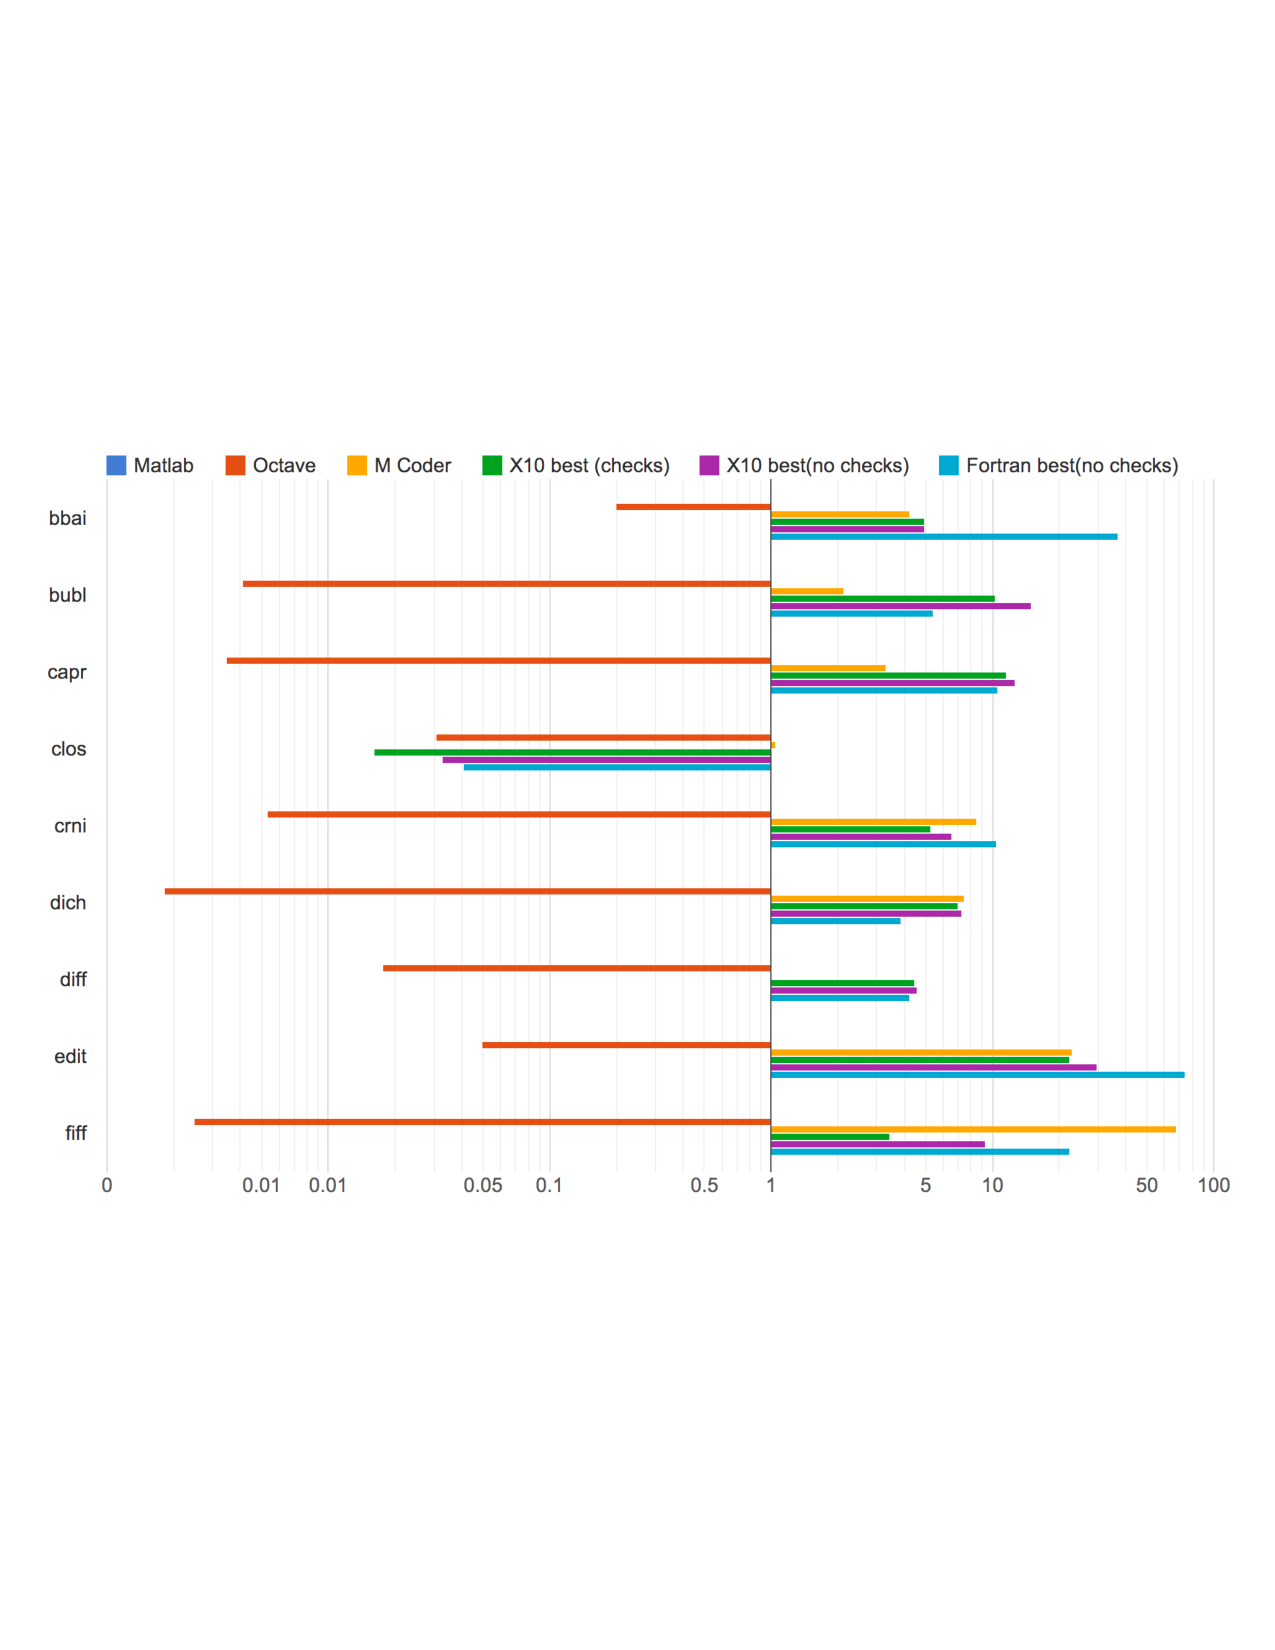
\includegraphics[width=\linewidth]{Figures/final/graph_1_1_1.pdf} \caption
{MiX10 performance comparison (part1) }\label{Fig:graph1_1_1} \end{center}
\end{figure} 
     
\begin{figure}[htbp] \begin{center}
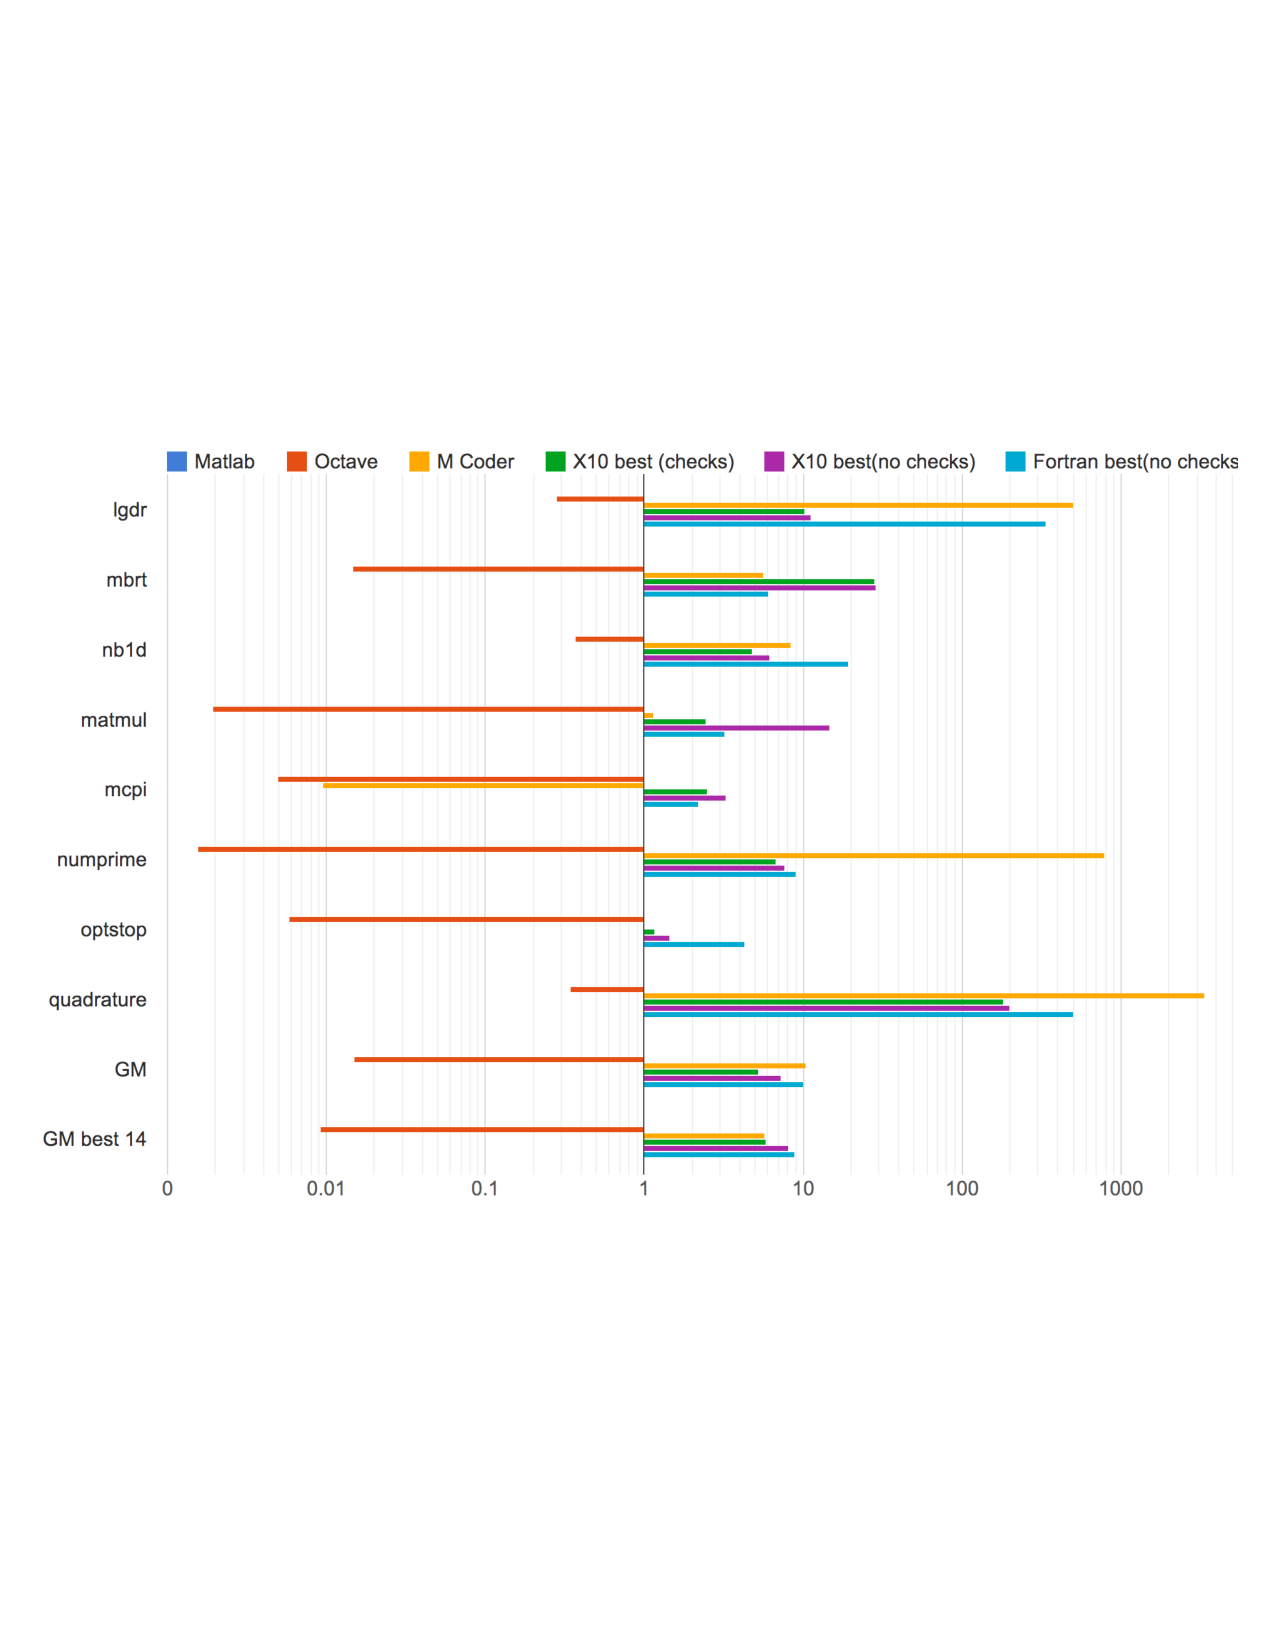
\includegraphics[width=\linewidth]{Figures/final/graph_1_1_2.pdf} \caption
{MiX10 performance comparison (part2) }\label{Fig:graph1_1_2} \end{center}
\end{figure} 

Figures \figref{Fig:graph1_1_1} and \figref{Fig:graph1_1_2} show the speedups
and slowdowns for codes generated for our benchmarks by different compilers.
For \mixten we have included results for generated \xten code by the
\emph{x10c++} compiler with 1) Array bounds checks turned off; and 2) Array
bounds checks turned on. We used the default optimization provided by the \xten
compiler (\texttt{-O}). For Fortran we included the code generated without
bounds checks. C code from \matlab coder was generated with default settings and
includes bounds checks. \figref{Fig:graph1_1_2} also shows the geometric mean of
speedups for all the benchmarks and for our best 14 out of 17 results (compared
to results from \matlab coder). 

We achieved a mean speedup of 5.2 and 7.2 for x10c++ with bounds checks and
x10c++ with no bounds checks respectively.  On the other hand \matlab coder gave
a mean speedup of 10.5 and \mctwofor gave a mean speedup of 10.2. However, we
see that if we do not consider only three benchmarks for which \xten does not
perform as well as C and Fortran, we get a mean sppedup of 5.75 for x10 with
bounds checks compared to 5.72 for C. For no bounds checks we get a mean speedup
of 8.1 compared to 8.8 for Fortran.  We outperform \matlab coder in 8 out of 17
benchmarks, and Fortran in 7 out of 17 benchmarks

\emph{clos} involves builtin matrix
multiplication operations for 2-dimensional matrices. The generated C code from
\matlab coder uses highly optimized matrix multiplication libraries compared to
the naive matrix multiplication implementation used by \mixten. Thus, we get a
speedup of 0.016 as compared to 1.049 for C. Note that the generated Fortran
code is also slowed down (speedup of 0.041) due to the same reason.        

\emph{lgdr} involves repeated transpose of a row vector to a column vector.
\matlab and Fortran, both being array languages are highly optimized for
transpose operations. \mixten currently uses a naive transpose algorithm which
is not as highly optimized. However, we still achieved a speedup of over 10 
times. 

\emph{quadrature} solves the stadard quadrature formula for numerical
integration~\cite{}, which involves repeated arithmetic calculations on a range
of numbers. We achieve a speedup of about 200 times compared to \matlab however
it is slow compared to speedups of 3348 and 502 by C and Fortran respectively.
We believe that \matlab coder leverages partial evaluation for optimizing
numerical methods' implementations.

Other interesting numbers are shown by \emph{optstop}, \emph{numprime} and
\emph{fiff}.
\emph{optstop} involves repeated array indexing by an index of type
\texttt{Double} which needs to be explicitly cast to \texttt{Long}, whenever
used as an index. IntegerOkay analysis cannot convert it to an integer type
because it's the value returned from a call to the \texttt{floor()} function
whose return type is \texttt{Double}. \emph{numprime} involves similar problem,
where the result of the \texttt{sqrt()} function needs to be converted to
\texttt{Long} from \texttt{Double}. \emph{numprime} also involves a for loop
over a conditional that evaluates to true only once. \matlab coder leverages
this fact for optimizing the for loop by implicitly inserting a \texttt{break}
when the conditional becomes true. We tested our generated \xten code by
explicitly inserting a \texttt{break} statement and achieved a speedup of around
65 times. Note that \emph{numprime} is also used for demonstrating
\texttt{parfor} which does not allow a \texttt{break} statement in the loop.
\emph{fiff} is characterized by stencil operations in a loop,
 on a 2-dimensional array. These operations are also optimized by array-based
languages like Fortran and \matlab.  
Note that for \emph{nb1d}, Fortran performs better due to the use of column
vectors in the benchmark, which are represented as 2-dimensional arrays in \xten
but in Fortran they are represented as 1-dimensional and are optimized.

For most of the other benchmarks, we perform better or nearly equal to C and
Fortran code. Inspite of the facts that 1) The sequential core of \xten is a
very high-level object oriented language which is not specialized for
array-based operations; and 2) Generating the executable binaries via \mixten
involves two levels of source-to-source compilations (\matlab $\rightarrow$
\xten $\rightarrow$ C++); We have achieved performance comparable to C and
Fortran.  
       



\chapter{Related work} \label{chap:Related}
There are several categories of related work.  First, we have the
immediate work upon which we are building.  The \mclab project already
provided the front-end and the \mcsaf\cite{JesseThesis} analysis
framework, which provided an important basis for the Tamer.  
Then there is \mcfor, a previous attempt to build a static
compiler targeting {\sc FORTRAN95}, that is part of the \mclab project.
There are also other compilers for \matlab, both static ones and
dynamic ones.
\
There is also related work on statically analyzing and compiling
other dynamic languages, with some similar problems we have faced,
and some similar approaches. Some of this work is presented
in section \secref{sec:otherStatic}.

\section{\mcfor}

We learned a lot from \mclab's previous \mcfor project\cite{McForThesis}
which was a first prototype \matlab to {\sc FORTRAN95}
compiler.  \mcfor supported a smaller subset of the language, and
simply ignored unsupported features - leading to possibly undefined
behavior. \mcfor did also not have a comprehensive approach to the
builtin functions, did not support the \matlab function lookup semantics, and
had a much more ad hoc approach to the analyses.  However, it really
showed that conversion of \matlab to {\sc FORTRAN95} was possible, and
that {\sc FORTRAN95} is an excellent target language.
In particular it showed that the numerical and matrix features
of {\sc FORTRAN95} are a good match for compiled \matlab, and that
the static nature of the language, together with powerful
{\sc FORTRAN95} compilers provide the potential for high performance.

We have developed the Tamer with targeting {\sc FORTRAN95} in mind. In
order to provide some extra flexibility for other potential backends
we have restricted \matlab less than may be necessary for a \matlab to
{\sc FORTRAN} compiler, i.e. it may have to restrict the \matlab
language further. For example, {\sc FORTRAN95} has very limited
polymorphism support, meaning that any polymorphic code can not be
easily \rednote{translated} to compact and readable FORTRAN. \mcfor does observe
these limitations, but does have an interesting way to deal with one
polymorphic case: If an if-statement results in incompatible types for
a variable along both branches, the code following that if-statement
gets copied into both branches, so that there won't be a confluence of
incompatible types.  For example,
\vspace{-.5cm}
\begin{lstlisting}
if (...)
  x = 3
else
  x = 'Hi'
end
foo(x)
\end{lstlisting}
may be converted to
\vspace{-.5cm}
\begin{lstlisting}
if (...)
  x = 3
  foo(x)
else
  x = 'Hi'
  foo(x)
end
\end{lstlisting}
This transformation is not possible in general for confluence points around
loop statements, and does also not work if values with ambiguous types
are returned from a function.

Despite being a full compiler with many interesting ideas, \mcfor is a
prototype, with limited feature set and limited extensibility. For
this thesis we have gone back to the basics and defined a much larger
subset of \matlab, taken a more structured and extensible approach to
building a general toolkit, tackled the problem of a principled
approach to the builtins, and defined the interprocedural analyses in
a more rigorous and extensible fashion.  The next generation of \mcfor
can now be built upon these new foundations.

\section{Other Static \matlab compilers}

Although we were not able to find publicly available versions, there
have been several excellent previous research projects on static
compilation of \matlab which focused particularly on the array-based
subset of \matlab and developed advanced static analyses for
determining shapes and sizes of arrays.  For example,
FALCON \cite{falcon} is a \matlab to {\sc FORTRAN90} translator with
sophisticated type inference algorithms.  Our Tamer is targeting a
larger and more modern set of \matlab that includes other types of
data structures such as cell arrays and structs, function handles and
lambda expressions, and which obeys the modern semantics of \matlab7.
We should note that FALCON handled interprocedural issues by fully
in-lining all of the the code.  MaJIC\cite{MaJIC}, a MATLAB
Just-In-Time compiler, is patterned after FALCON.  It uses similar
type inference techniques to FALCON, but are simplified to fit the JIT
context.  MAGICA \cite{Joisha03,MAGICA} is a type inference engine
developed by Joisha and Banerjee of Northwestern University, and is
written in Mathematica and is designed as an add-on module used by
MAT2C compiler \cite{MAT2C}.  We hope to learn from the advanced type
inference approaches in these projects and to implement similar
approximations using our interprocedural value analysis.

There are also commercial compilers, which are not publicly available, and for
which there are no research articles.   One such product is the \textit{MATLABCoder} 
recently released by MathWorks\cite{MATLABCoder}.   This product
produces C code for a subset of \matlab.  According to our preliminary tests,
this product does not appear to support cell arrays except in very
specific circumstances, nor does it support a general form of lambda
expressions, and was therefore unable to handle quite a few of our benchmarks.  
However, the key differences with our work is that we are
designing and providing an extensible and open source toolkit for compiler and
tool researchers.   This is clearly not the main goal of proprietary compilers.

\section{Other \matlab-like systems}

There are other projects providing open source implementations of \matlab-like
languages, such as Octave\cite{Octave} and Scilab\cite{Scilab}.   Although
these add valuable contributions to the open source community,  
their focus is on providing interpreters and open library support and they have
not tackled the problems of static compilation.   Thus, we believe that our
contributions are complementary. In particular Octave may present opportunities
to improve the usefulness of our static compiler framework without requiring
an actual \matlab installation.
 Octave, being an interpreter system, may not provide very high
performance, but it does include a large library similar to \matlab's
library. Enabling our framework to support Octave's specific \matlab flavor
may help bring together Octave's completeness with the potential performance
gains of a static compilation framework.


\section{Static Approaches to other Dynamic Languages}
\label{sec:otherStatic}

Other dynamic languages have had very successful efforts in defining
static subsets in order to provide static analysis.

\subsection{Python}

Reduced Python (RPython)\cite{RPython} provided inspiration for our
approach at dealing with a dynamic language in a static way. Rather
than attempting to support dynamic features that are not amenable to
static compilation, for example by providing interpreter-like features
as a fallback, RPython restricts (``reduces'') the set of allowable features such
that programs are statically typable. At the same time, it attempts to
stay as expressive as possible.

RPython was originally developed for PyPy, a Python interpreter written \rednote{in} Python,
but has evolved into be a general purpose language.
It was not developed to compile programs completely statically,
but rather with the goal to speed up execution times in 
virtual machines like VM or CLI, which are themselves developed
for static languages (Java and C\#, respectively).

%boot strapping phase?

Besides disallowing dynamic features, RPython disallows a basic feature
of many dynamic programing languages: at a confluence point,
a variable may not be defined with two incompatible types. This
notion that a variable should have one specific type at every programming
point is something that we expect for static backends of our framework
as well, in particular for FORTRAN, even if the Tamer Framework itself
actually supports union types. Both RPython, as well as our own research
have indicated that this restriction is not a serious limitation in practice.

RPython restricts Python's container types. In particular, it forces
that dictionaries (hash-tables) and arrays are homogeneous, i.e. all
elements have the same type. Tuples are allowed to be inhomogeneous.
For the Tamer, we represent the two builtin container types (structs,
cells) in both possible ways: as a tuple or as a collection, which correspond to
inhomogeneous and homogeneous representations, respectively.

RPython does not directly support generic functions, i.e. if a function
is used multiple times with incompatible arguments, the program
gets rejected. The Tamer uses a context-sensitive interprocedural
analysis that creates copies of functions when they are called
with incompatible arguments.


\subsection{Ruby}
DiamondbackRuby (DRuby) is a static type inference toolkit for Ruby
\cite{StaticRuby}, mostly with the goal to gain the advantage of static languages
to report potential errors ahead of time.  Ruby, like \matlab, is a
dynamic, interpreted language, but is used more in web
development. Some of the approaches of DRuby are similar to the Tamer
framework.

Similar to \matlab, the core library of Ruby is written in native code
(i.e. in C), rather than Ruby itself - which may also have different
behaviors depending on the incoming argument types. Thus DRuby has to
provide type information for builtin functions. In order to that,
DRuby includes a type annotation language, which can also be used to
specify types for functions with difficult behavior. Note that at this
point, the focus of our builtin framework is to organize the large
number of builtins, but our work may lead to a proper type annotation
language as well.

DRuby also provides a type inference, but it is based on a
constraint-based analysis. DRuby constrains the set of supported
language features to enable the static analysis, but allows some of
them by inserting runtime checks to still be able to support them.
These are included in such a way as to help users identify where
exactly the error occurred.

Using the results of the static analyses provided by the \matlab Tamer
to provide information about potential runtime errors is one
of the possible goals of continued research.


\chapter{Conclusions and Future Work} \label{chap:Conclusions}
This thesis has introduced the \matlab Tamer, an extensible
object-oriented framework for supporting the translation from
dynamic \matlab programs to a Tame IR, call graph and class/type
information suitable for generating static code.  We provided an
introduction to the features of \matlab in a form that we believe
helps expose the semantics of mclasses and function lookup for
compiler and tool writers, and should help motivate some of the
restrictions we impose on the language.  We tackled the somewhat
daunting problem of handling the large number of builtin functions
in \matlab by defining an extensible hierarchy of builtins and a small
domain-specific language to define their behavior.  We defined a Tame
IR and added functionality to \mcsaf to produce the IR and to extend
the analysis framework to handle \rednote{the} new IR nodes introduced.  We
provided an interprocedural analysis framework that allows creation of
full-program analyses of \matlab programs.  Finally, we developed an
extensible value estimation analysis that we use to provide a
callgraph constructor for \matlab programs, using the proper
lookup semantics, starting with some entry point.

\section{Future Work}

Our initial experiments with the framework are very encouraging and there
are several possible projects to continue the development of
static compilers for \matlab as part of the \mclab project.
We also hope that others will also use Tamer the framework for a
variety of static \matlab tools.


In the following we will present some ideas
for the continued development of the static portion of the \mclab framework.

%We also plan to continue developing the value analysis to add richer
%abstractions for shape and other data structure properties.  Finally, as a part
%of a larger project on benchmarking \matlab, we hope to expand our set of
%benchmarks and to further examine which features might be tamed, and to extend
%our set of automated refactorings.

The major goal of the Tamer Framework is to provide a starting point for
compiler backends targeting static programming languages. In particular,
we have developed our toolkit with compilation targeting 
 {\sc FORTRAN95} in mind. In order to actually be able to compile,
the abstract value representations need to be further refined, and the value
analysis extended. In particular, shape information for arrays is needed,
which may be dealt with in a similar way as the mclass information.
Further refinement of the value representations can improve the supported feature
set and performance. For example, having exact knowledge whether numerical
values may be real, complex or imaginary allows using complex data types only
when necessary, rather than using complex numbers by default for all values.
Advanced analyses could be used to the relationships of array-shapes and
values of variables, enabling the removal of run-time array bounds checks.
This may provide significant performance benefits.

Further work may focus around expanding the set of supported \matlab features.
Interesting may be the extension of the Tamer framework to fully support
\matlab user-defined classes, including the ``old'' semantics, the ``new''
semantics since version 7.6, and possibly \rednote{handle-classes}. The \matlab Tamer
already supports the notions of mclasses, and the overloading semantics
necessary to implement class semantics are already supported. Note that in order
to support \rednote{handle-classes}, it is not sufficient to extend the value representations -
the machinery of the analysis also has to be extended \rednote{to} capture changes of
arguments that use the reference semantics of \rednote{handle-classes}. This is also
true if the Tame \matlab language subset was extended to support global and
persistent variables.

The Tamer framework could work together with \mclab's refactoring
tools in two ways. For one it would be possible to use the
refactorings as code transformations in a pre-processing step, to be
able to reduce/refactor some unsupported dynamic feature
of \matlab. For example, the refactoring toolkit allows
transforming \matlab scripts into \matlab functions. Another way the
refactoring tools could work together with the Tamer framework is in
an interactive fashion. A user wishing to compile a program
may find that the Tamer rejects it; the refactoring toolkit could
then step in and suggest to refactor the program in certain ways
to make it possible to compile.

Future work may advance the static compilation framework and the
notion of bridging the gap between dynamic languages and static
analyses and compilation.  The builtin framework with its approach to
allow the explicit and compact definition of flow information for functions
may lead to a general type annotation language for \matlab types, which could
be used both to type builtin functions, or to type user and library
functions with complex behavior. Static information provided by full-program
analyses using these frameworks could be used to find potential
runtime errors, and aid programmers build better and more correct programs.







\appendix % -- Appendices -----------------------------------------------------

\addtocontents{toc}{\protect\addvspace{10pt}}
\addtocontents{toc}{\protect\contentsline{part}{Appendices}{}{}}
% -> extra {} for hyperref
%\label{TODO} % stub label for undetermined ref

\chapter{XML structure for builtin framework} \label{chap:Builtinxml}
In the following we provide a list of \matlab builtin functions.
The corresponding numbers show how many callsites there are for the function
within the large set of \matlab programs that can be analyzed by the \mcbench framework.

When selecting the initial set of builtin functions for the 
builtin framework, we use most of the below functions, excluding
dynamic and GUI functions. We added functions corresponding
to \matlab operators, as well as some \rednote{functions} that are very
closely related to functions in the list.

%\secref{sec:idBuiltins}
\begin{table}
\caption[List of builtins and their frequency of occurrence]{List of builtins and their frequency of occurrence (continued on the following pages)}
\end{table}
\begin{footnotesize}
%\begin {tabular} {|l|l|} % \hline
\vspace{-.153cm}
\begin{multicols}{3}
\noindent
\vspace{-.153cm} 1     \hspace{.2cm} {\tt recycle             }   \\ % \hline
\vspace{-.153cm} 1     \hspace{.2cm} {\tt schur               }   \\ % \hline
\vspace{-.153cm} 1     \hspace{.2cm} {\tt gt                  }   \\ % \hline
\vspace{-.153cm} 1     \hspace{.2cm} {\tt mislocked           }   \\ % \hline
\vspace{-.153cm} 1     \hspace{.2cm} {\tt acotd               }   \\ % \hline
\vspace{-.153cm} 1     \hspace{.2cm} {\tt more                }   \\ % \hline
\vspace{-.153cm} 1     \hspace{.2cm} {\tt acot                }   \\ % \hline
\vspace{-.153cm} 1     \hspace{.2cm} {\tt uminus              }   \\ % \hline
\vspace{-.153cm} 1     \hspace{.2cm} {\tt uitoolbar           }   \\ % \hline
\vspace{-.153cm} 1     \hspace{.2cm} {\tt dbclear             }   \\ % \hline
\vspace{-.153cm} 1     \hspace{.2cm} {\tt isjava              }   \\ % \hline
\vspace{-.153cm} 1     \hspace{.2cm} {\tt ordschur            }   \\ % \hline
\vspace{-.153cm} 1     \hspace{.2cm} {\tt munlock             }   \\ % \hline
\vspace{-.153cm} 1     \hspace{.2cm} {\tt superiorto          }   \\ % \hline
\vspace{-.153cm} 1     \hspace{.2cm} {\tt unicode2native      }   \\ % \hline
\vspace{-.153cm} 1     \hspace{.2cm} {\tt methods             }   \\ % \hline
\vspace{-.153cm} 1     \hspace{.2cm} {\tt dmperm              }   \\ % \hline
\vspace{-.153cm} 1     \hspace{.2cm} {\tt fileattrib          }   \\ % \hline
\vspace{-.153cm} 1     \hspace{.2cm} {\tt delaunay            }   \\ % \hline
\vspace{-.153cm} 1     \hspace{.2cm} {\tt isequalwithequalnans}   \\ % \hline
\vspace{-.153cm} 1     \hspace{.2cm} {\tt javaMethod          }   \\ % \hline
\vspace{-.153cm} 1     \hspace{.2cm} {\tt functions           }   \\ % \hline
\vspace{-.153cm} 1     \hspace{.2cm} {\tt structfun           }   \\ % \hline
\vspace{-.153cm} 2     \hspace{.2cm} {\tt subsasgn            }   \\ % \hline
\vspace{-.153cm} 2     \hspace{.2cm} {\tt rehash              }   \\ % \hline
\vspace{-.153cm} 2     \hspace{.2cm} {\tt ne                  }   \\ % \hline
\vspace{-.153cm} 2     \hspace{.2cm} {\tt linsolve            }   \\ % \hline
\vspace{-.153cm} 2     \hspace{.2cm} {\tt regexptranslate     }   \\ % \hline
\vspace{-.153cm} 2     \hspace{.2cm} {\tt memory              }   \\ % \hline
\vspace{-.153cm} 2     \hspace{.2cm} {\tt uitable             }   \\ % \hline
\vspace{-.153cm} 2     \hspace{.2cm} {\tt matlabpath          }   \\ % \hline
\vspace{-.153cm} 2     \hspace{.2cm} {\tt exit                }   \\ % \hline
\vspace{-.153cm} 2     \hspace{.2cm} {\tt ge                  }   \\ % \hline
\vspace{-.153cm} 2     \hspace{.2cm} {\tt uint64              }   \\ % \hline
\vspace{-.153cm} 2     \hspace{.2cm} {\tt atanh               }   \\ % \hline
\vspace{-.153cm} 2     \hspace{.2cm} {\tt ishghandle          }   \\ % \hline
\vspace{-.153cm} 2     \hspace{.2cm} {\tt cotd                }   \\ % \hline
\vspace{-.153cm} 2     \hspace{.2cm} {\tt isdeployed          }   \\ % \hline
\vspace{-.153cm} 2     \hspace{.2cm} {\tt le                  }   \\ % \hline
\vspace{-.153cm} 2     \hspace{.2cm} {\tt prefdir             }   \\ % \hline
\vspace{-.153cm} 3     \hspace{.2cm} {\tt isstrprop           }   \\ % \hline
\vspace{-.153cm} 3     \hspace{.2cm} {\tt dragrect            }   \\ % \hline
\vspace{-.153cm} 3     \hspace{.2cm} {\tt uitoggletool        }   \\ % \hline
\vspace{-.153cm} 3     \hspace{.2cm} {\tt ferror              }   \\ % \hline
\vspace{-.153cm} 3     \hspace{.2cm} {\tt javaArray           }   \\ % \hline
\vspace{-.153cm} 3     \hspace{.2cm} {\tt javaObject          }   \\ % \hline
\vspace{-.153cm} 3     \hspace{.2cm} {\tt sec                 }   \\ % \hline
\vspace{-.153cm} 3     \hspace{.2cm} {\tt hgconvertunits      }   \\ % \hline
\vspace{-.153cm} 3     \hspace{.2cm} {\tt pack                }   \\ % \hline
\vspace{-.153cm} 3     \hspace{.2cm} {\tt sortrowsc           }   \\ % \hline
\vspace{-.153cm} 3     \hspace{.2cm} {\tt lt                  }   \\ % \hline
\vspace{-.153cm} 3     \hspace{.2cm} {\tt echo                }   \\ % \hline
\vspace{-.153cm} 4     \hspace{.2cm} {\tt validatestring      }   \\ % \hline
\vspace{-.153cm} 4     \hspace{.2cm} {\tt tand                }   \\ % \hline
\vspace{-.153cm} 4     \hspace{.2cm} {\tt dbstop              }   \\ % \hline
\vspace{-.153cm} 4     \hspace{.2cm} {\tt int64               }   \\ % \hline
\vspace{-.153cm} 4     \hspace{.2cm} {\tt csc                 }   \\ % \hline
\vspace{-.153cm} 4     \hspace{.2cm} {\tt hardcopy            }   \\ % \hline
\vspace{-.153cm} 4     \hspace{.2cm} {\tt uipushtool          }   \\ % \hline
\vspace{-.153cm} 4     \hspace{.2cm} {\tt asinh               }   \\ % \hline
\vspace{-.153cm} 4     \hspace{.2cm} {\tt asind               }   \\ % \hline
\vspace{-.153cm} 5     \hspace{.2cm} {\tt native2unicode      }   \\ % \hline
\vspace{-.153cm} 5     \hspace{.2cm} {\tt erf                 }   \\ % \hline
\vspace{-.153cm} 5     \hspace{.2cm} {\tt who                 }   \\ % \hline
\vspace{-.153cm} 5     \hspace{.2cm} {\tt hggroup             }   \\ % \hline
\vspace{-.153cm} 5     \hspace{.2cm} {\tt rbbox               }   \\ % \hline
\vspace{-.153cm} 5     \hspace{.2cm} {\tt bitor               }   \\ % \hline
\vspace{-.153cm} 5     \hspace{.2cm} {\tt erfinv              }   \\ % \hline
\vspace{-.153cm} 5     \hspace{.2cm} {\tt lu                  }   \\ % \hline
\vspace{-.153cm} 5     \hspace{.2cm} {\tt colstyle            }   \\ % \hline
\vspace{-.153cm} 5     \hspace{.2cm} {\tt im2frame            }   \\ % \hline
\vspace{-.153cm} 6     \hspace{.2cm} {\tt frame2im            }   \\ % \hline
\vspace{-.153cm} 6     \hspace{.2cm} {\tt ifftn               }   \\ % \hline
\vspace{-.153cm} 6     \hspace{.2cm} {\tt hgtransform         }   \\ % \hline
\vspace{-.153cm} 6     \hspace{.2cm} {\tt diary               }   \\ % \hline
\vspace{-.153cm} 6     \hspace{.2cm} {\tt subsref             }   \\ % \hline
\vspace{-.153cm} 6     \hspace{.2cm} {\tt erfcinv             }   \\ % \hline
\vspace{-.153cm} 6     \hspace{.2cm} {\tt rcond               }   \\ % \hline
\vspace{-.153cm} 6     \hspace{.2cm} {\tt home                }   \\ % \hline
\vspace{-.153cm} 7     \hspace{.2cm} {\tt uicontextmenu       }   \\ % \hline
\vspace{-.153cm} 7     \hspace{.2cm} {\tt cot                 }   \\ % \hline
\vspace{-.153cm} 7     \hspace{.2cm} {\tt reset               }   \\ % \hline
\vspace{-.153cm} 7     \hspace{.2cm} {\tt eq                  }   \\ % \hline
\vspace{-.153cm} 7     \hspace{.2cm} {\tt sech                }   \\ % \hline
\vspace{-.153cm} 7     \hspace{.2cm} {\tt builtin             }   \\ % \hline
\vspace{-.153cm} 8     \hspace{.2cm} {\tt type                }   \\ % \hline
\vspace{-.153cm} 8     \hspace{.2cm} {\tt setstr              }   \\ % \hline
\vspace{-.153cm} 8     \hspace{.2cm} {\tt validateattributes  }   \\ % \hline
\vspace{-.153cm} 8     \hspace{.2cm} {\tt what                }   \\ % \hline
\vspace{-.153cm} 8     \hspace{.2cm} {\tt atand               }   \\ % \hline
\vspace{-.153cm} 9     \hspace{.2cm} {\tt issorted            }   \\ % \hline
\vspace{-.153cm} 9     \hspace{.2cm} {\tt acosh               }   \\ % \hline
\vspace{-.153cm} 9     \hspace{.2cm} {\tt int8                }   \\ % \hline
\vspace{-.153cm} 9     \hspace{.2cm} {\tt light               }   \\ % \hline
\vspace{-.153cm} 9     \hspace{.2cm} {\tt betainc             }   \\ % \hline
\vspace{-.153cm} 10    \hspace{.2cm} {\tt keyboard            }    \\ % \hline
\vspace{-.153cm} 11    \hspace{.2cm} {\tt rethrow             }    \\ % \hline
\vspace{-.153cm} 11    \hspace{.2cm} {\tt fftn                }    \\ % \hline
\vspace{-.153cm} 11    \hspace{.2cm} {\tt feof                }    \\ % \hline
\vspace{-.153cm} 11    \hspace{.2cm} {\tt rmdir               }    \\ % \hline
\vspace{-.153cm} 11    \hspace{.2cm} {\tt libisloaded         }    \\ % \hline
\vspace{-.153cm} 11    \hspace{.2cm} {\tt isletter            }    \\ % \hline
\vspace{-.153cm} 11    \hspace{.2cm} {\tt cast                }    \\ % \hline
\vspace{-.153cm} 11    \hspace{.2cm} {\tt unloadlibrary       }    \\ % \hline
\vspace{-.153cm} 11    \hspace{.2cm} {\tt evalc               }    \\ % \hline
\vspace{-.153cm} 12    \hspace{.2cm} {\tt waitfor             }    \\ % \hline
\vspace{-.153cm} 12    \hspace{.2cm} {\tt power               }    \\ % \hline
\vspace{-.153cm} 12    \hspace{.2cm} {\tt isvarname           }    \\ % \hline
\vspace{-.153cm} 12    \hspace{.2cm} {\tt loglog              }    \\ % \hline
\vspace{-.153cm} 12    \hspace{.2cm} {\tt pow2                }    \\ % \hline
\vspace{-.153cm} 13    \hspace{.2cm} {\tt convhull            }    \\ % \hline
\vspace{-.153cm} 13    \hspace{.2cm} {\tt mexext              }    \\ % \hline
\vspace{-.153cm} 13    \hspace{.2cm} {\tt speye               }    \\ % \hline
\vspace{-.153cm} 13    \hspace{.2cm} {\tt vertcat             }    \\ % \hline
\vspace{-.153cm} 13    \hspace{.2cm} {\tt int16               }    \\ % \hline
\vspace{-.153cm} 13    \hspace{.2cm} {\tt getenv              }    \\ % \hline
\vspace{-.153cm} 14    \hspace{.2cm} {\tt func2str            }    \\ % \hline
\vspace{-.153cm} 14    \hspace{.2cm} {\tt acosd               }    \\ % \hline
\vspace{-.153cm} 14    \hspace{.2cm} {\tt lasterror           }    \\ % \hline
\vspace{-.153cm} 14    \hspace{.2cm} {\tt movefile            }    \\ % \hline
\vspace{-.153cm} 15    \hspace{.2cm} {\tt isspace             }    \\ % \hline
\vspace{-.153cm} 15    \hspace{.2cm} {\tt isinteger           }    \\ % \hline
\vspace{-.153cm} 15    \hspace{.2cm} {\tt randi               }    \\ % \hline
\vspace{-.153cm} 15    \hspace{.2cm} {\tt horzcat             }    \\ % \hline
\vspace{-.153cm} 16    \hspace{.2cm} {\tt gammainc            }    \\ % \hline
\vspace{-.153cm} 16    \hspace{.2cm} {\tt regexpi             }    \\ % \hline
\vspace{-.153cm} 17    \hspace{.2cm} {\tt accumarray          }    \\ % \hline
\vspace{-.153cm} 17    \hspace{.2cm} {\tt dbstack             }    \\ % \hline
\vspace{-.153cm} 17    \hspace{.2cm} {\tt hypot               }    \\ % \hline
\vspace{-.153cm} 17    \hspace{.2cm} {\tt isappdata           }    \\ % \hline
\vspace{-.153cm} 17    \hspace{.2cm} {\tt or                  }    \\ % \hline
\vspace{-.153cm} 18    \hspace{.2cm} {\tt whos                }    \\ % \hline
\vspace{-.153cm} 19    \hspace{.2cm} {\tt unix                }    \\ % \hline
\vspace{-.153cm} 19    \hspace{.2cm} {\tt tril                }    \\ % \hline
\vspace{-.153cm} 19    \hspace{.2cm} {\tt inputname           }    \\ % \hline
\vspace{-.153cm} 19    \hspace{.2cm} {\tt copyfile            }    \\ % \hline
\vspace{-.153cm} 19    \hspace{.2cm} {\tt qr                  }    \\ % \hline
\vspace{-.153cm} 20    \hspace{.2cm} {\tt cell2struct         }    \\ % \hline
\vspace{-.153cm} 20    \hspace{.2cm} {\tt isobject            }    \\ % \hline
\vspace{-.153cm} 23    \hspace{.2cm} {\tt ancestor            }    \\ % \hline
\vspace{-.153cm} 23    \hspace{.2cm} {\tt handle              }    \\ % \hline
\vspace{-.153cm} 24    \hspace{.2cm} {\tt issparse            }    \\ % \hline
\vspace{-.153cm} 24    \hspace{.2cm} {\tt bitset              }    \\ % \hline
\vspace{-.153cm} 25    \hspace{.2cm} {\tt and                 }    \\ % \hline
\vspace{-.153cm} 25    \hspace{.2cm} {\tt lastwarn            }    \\ % \hline
\vspace{-.153cm} 26    \hspace{.2cm} {\tt bitand              }    \\ % \hline
\vspace{-.153cm} 26    \hspace{.2cm} {\tt nonzeros            }    \\ % \hline
\vspace{-.153cm} 26    \hspace{.2cm} {\tt matlabroot          }    \\ % \hline
\vspace{-.153cm} 26    \hspace{.2cm} {\tt chol                }    \\ % \hline
\vspace{-.153cm} 27    \hspace{.2cm} {\tt typecast            }    \\ % \hline
\vspace{-.153cm} 27    \hspace{.2cm} {\tt rmappdata           }    \\ % \hline
\vspace{-.153cm} 27    \hspace{.2cm} {\tt cumprod             }    \\ % \hline
\vspace{-.153cm} 27    \hspace{.2cm} {\tt struct2cell         }    \\ % \hline
\vspace{-.153cm} 28    \hspace{.2cm} {\tt isfloat             }    \\ % \hline
\vspace{-.153cm} 29    \hspace{.2cm} {\tt nnz                 }    \\ % \hline
\vspace{-.153cm} 29    \hspace{.2cm} {\tt bitget              }    \\ % \hline
\vspace{-.153cm} 29    \hspace{.2cm} {\tt uint32              }    \\ % \hline
\vspace{-.153cm} 29    \hspace{.2cm} {\tt ftell               }    \\ % \hline
\vspace{-.153cm} 29    \hspace{.2cm} {\tt cosh                }    \\ % \hline
\vspace{-.153cm} 30    \hspace{.2cm} {\tt surface             }    \\ % \hline
\vspace{-.153cm} 31    \hspace{.2cm} {\tt waitforbuttonpress  }    \\ % \hline
\vspace{-.153cm} 31    \hspace{.2cm} {\tt fgets               }    \\ % \hline
\vspace{-.153cm} 31    \hspace{.2cm} {\tt realsqrt            }    \\ % \hline
\vspace{-.153cm} 33    \hspace{.2cm} {\tt rectangle           }    \\ % \hline
\vspace{-.153cm} 33    \hspace{.2cm} {\tt arrayfun            }    \\ % \hline
\vspace{-.153cm} 34    \hspace{.2cm} {\tt tanh                }    \\ % \hline
\vspace{-.153cm} 34    \hspace{.2cm} {\tt bitshift            }    \\ % \hline
\vspace{-.153cm} 34    \hspace{.2cm} {\tt semilogy            }    \\ % \hline
\vspace{-.153cm} 34    \hspace{.2cm} {\tt nargoutchk          }    \\ % \hline
\vspace{-.153cm} 35    \hspace{.2cm} {\tt asin                }    \\ % \hline
\vspace{-.153cm} 35    \hspace{.2cm} {\tt mkdir               }    \\ % \hline
\vspace{-.153cm} 35    \hspace{.2cm} {\tt int32               }    \\ % \hline
\vspace{-.153cm} 36    \hspace{.2cm} {\tt textscan            }    \\ % \hline
\vspace{-.153cm} 36    \hspace{.2cm} {\tt svd                 }    \\ % \hline
\vspace{-.153cm} 36    \hspace{.2cm} {\tt sinh                }    \\ % \hline
\vspace{-.153cm} 36    \hspace{.2cm} {\tt lasterr             }    \\ % \hline
\vspace{-.153cm} 36    \hspace{.2cm} {\tt computer            }    \\ % \hline
\vspace{-.153cm} 38    \hspace{.2cm} {\tt version             }    \\ % \hline
\vspace{-.153cm} 40    \hspace{.2cm} {\tt cosd                }    \\ % \hline
\vspace{-.153cm} 41    \hspace{.2cm} {\tt xor                 }    \\ % \hline
\vspace{-.153cm} 43    \hspace{.2cm} {\tt sind                }    \\ % \hline
\vspace{-.153cm} 44    \hspace{.2cm} {\tt beep                }    \\ % \hline
\vspace{-.153cm} 45    \hspace{.2cm} {\tt triu                }    \\ % \hline
\vspace{-.153cm} 45    \hspace{.2cm} {\tt gammaln             }    \\ % \hline
\vspace{-.153cm} 47    \hspace{.2cm} {\tt copyobj             }    \\ % \hline
\vspace{-.153cm} 49    \hspace{.2cm} {\tt fill3               }    \\ % \hline
\vspace{-.153cm} 49    \hspace{.2cm} {\tt islogical           }    \\ % \hline
\vspace{-.153cm} 51    \hspace{.2cm} {\tt semilogx            }    \\ % \hline
\vspace{-.153cm} 51    \hspace{.2cm} {\tt histc               }    \\ % \hline
\vspace{-.153cm} 55    \hspace{.2cm} {\tt uint16              }    \\ % \hline
\vspace{-.153cm} 55    \hspace{.2cm} {\tt gamma               }    \\ % \hline
\vspace{-.153cm} 55    \hspace{.2cm} {\tt system              }    \\ % \hline
\vspace{-.153cm} 56    \hspace{.2cm} {\tt uipanel             }    \\ % \hline
\vspace{-.153cm} 60    \hspace{.2cm} {\tt dos                 }    \\ % \hline
\vspace{-.153cm} 60    \hspace{.2cm} {\tt transpose           }    \\ % \hline
\vspace{-.153cm} 61    \hspace{.2cm} {\tt complex             }    \\ % \hline
\vspace{-.153cm} 62    \hspace{.2cm} {\tt format              }    \\ % \hline
\vspace{-.153cm} 66    \hspace{.2cm} {\tt acos                }    \\ % \hline
\vspace{-.153cm} 67    \hspace{.2cm} {\tt erfc                }    \\ % \hline
\vspace{-.153cm} 68    \hspace{.2cm} {\tt calllib             }    \\ % \hline
\vspace{-.153cm} 69    \hspace{.2cm} {\tt strncmpi            }    \\ % \hline
\vspace{-.153cm} 70    \hspace{.2cm} {\tt strtrim             }    \\ % \hline
\vspace{-.153cm} 74    \hspace{.2cm} {\tt det                 }    \\ % \hline
\vspace{-.153cm} 76    \hspace{.2cm} {\tt atan                }    \\ % \hline
\vspace{-.153cm} 76    \hspace{.2cm} {\tt import              }    \\ % \hline
\vspace{-.153cm} 82    \hspace{.2cm} {\tt isstruct            }    \\ % \hline
\vspace{-.153cm} 82    \hspace{.2cm} {\tt sscanf              }    \\ % \hline
\vspace{-.153cm} 85    \hspace{.2cm} {\tt isstr               }    \\ % \hline
\vspace{-.153cm} 86    \hspace{.2cm} {\tt not                 }    \\ % \hline
\vspace{-.153cm} 90    \hspace{.2cm} {\tt full                }    \\ % \hline
\vspace{-.153cm} 91    \hspace{.2cm} {\tt strncmp             }    \\ % \hline
\vspace{-.153cm} 92    \hspace{.2cm} {\tt eig                 }    \\ % \hline
\vspace{-.153cm} 93    \hspace{.2cm} {\tt log2                }    \\ % \hline
\vspace{-.153cm} 93    \hspace{.2cm} {\tt regexprep           }    \\ % \hline
\vspace{-.153cm} 94    \hspace{.2cm} {\tt permute             }    \\ % \hline
\vspace{-.153cm} 95    \hspace{.2cm} {\tt which               }    \\ % \hline
\vspace{-.153cm} 96    \hspace{.2cm} {\tt class               }    \\ % \hline
\vspace{-.153cm} 97    \hspace{.2cm} {\tt tan                 }    \\ % \hline
\vspace{-.153cm} 101   \hspace{.2cm} {\tt isinf               }     \\ % \hline
\vspace{-.153cm} 103   \hspace{.2cm} {\tt bitxor              }     \\ % \hline
\vspace{-.153cm} 105   \hspace{.2cm} {\tt upper               }     \\ % \hline
\vspace{-.153cm} 105   \hspace{.2cm} {\tt ifft                }     \\ % \hline
\vspace{-.153cm} 105   \hspace{.2cm} {\tt isvector            }     \\ % \hline
\vspace{-.153cm} 106   \hspace{.2cm} {\tt fieldnames          }     \\ % \hline
\vspace{-.153cm} 109   \hspace{.2cm} {\tt fill                }     \\ % \hline
\vspace{-.153cm} 114   \hspace{.2cm} {\tt filter              }     \\ % \hline
\vspace{-.153cm} 117   \hspace{.2cm} {\tt cputime             }     \\ % \hline
\vspace{-.153cm} 119   \hspace{.2cm} {\tt fseek               }     \\ % \hline
\vspace{-.153cm} 124   \hspace{.2cm} {\tt assert              }     \\ % \hline
\vspace{-.153cm} 125   \hspace{.2cm} {\tt image               }     \\ % \hline
\vspace{-.153cm} 131   \hspace{.2cm} {\tt bsxfun              }     \\ % \hline
\vspace{-.153cm} 131   \hspace{.2cm} {\tt regexp              }     \\ % \hline
\vspace{-.153cm} 131   \hspace{.2cm} {\tt conv2               }     \\ % \hline
\vspace{-.153cm} 137   \hspace{.2cm} {\tt evalin              }     \\ % \hline
\vspace{-.153cm} 137   \hspace{.2cm} {\tt assignin            }     \\ % \hline
\vspace{-.153cm} 142   \hspace{.2cm} {\tt sparse              }     \\ % \hline
\vspace{-.153cm} 146   \hspace{.2cm} {\tt dir                 }     \\ % \hline
\vspace{-.153cm} 154   \hspace{.2cm} {\tt clc                 }     \\ % \hline
\vspace{-.153cm} 157   \hspace{.2cm} {\tt logical             }     \\ % \hline
\vspace{-.153cm} 158   \hspace{.2cm} {\tt isscalar            }     \\ % \hline
\vspace{-.153cm} 164   \hspace{.2cm} {\tt cat                 }     \\ % \hline
\vspace{-.153cm} 166   \hspace{.2cm} {\tt patch               }     \\ % \hline
\vspace{-.153cm} 170   \hspace{.2cm} {\tt isfinite            }     \\ % \hline
\vspace{-.153cm} 171   \hspace{.2cm} {\tt deblank             }     \\ % \hline
\vspace{-.153cm} 173   \hspace{.2cm} {\tt plot3               }     \\ % \hline
\vspace{-.153cm} 174   \hspace{.2cm} {\tt atan2               }     \\ % \hline
\vspace{-.153cm} 176   \hspace{.2cm} {\tt cellfun             }     \\ % \hline
\vspace{-.153cm} 180   \hspace{.2cm} {\tt feval               }     \\ % \hline
\vspace{-.153cm} 183   \hspace{.2cm} {\tt fscanf              }     \\ % \hline
\vspace{-.153cm} 183   \hspace{.2cm} {\tt inv                 }     \\ % \hline
\vspace{-.153cm} 193   \hspace{.2cm} {\tt save                }     \\ % \hline
\vspace{-.153cm} 199   \hspace{.2cm} {\tt strfind             }     \\ % \hline
\vspace{-.153cm} 204   \hspace{.2cm} {\tt fwrite              }     \\ % \hline
\vspace{-.153cm} 204   \hspace{.2cm} {\tt ndims               }     \\ % \hline
\vspace{-.153cm} 210   \hspace{.2cm} {\tt cumsum              }     \\ % \hline
\vspace{-.153cm} 213   \hspace{.2cm} {\tt ishandle            }     \\ % \hline
\vspace{-.153cm} 213   \hspace{.2cm} {\tt rem                 }     \\ % \hline
\vspace{-.153cm} 214   \hspace{.2cm} {\tt nargchk             }     \\ % \hline
\vspace{-.153cm} 222   \hspace{.2cm} {\tt fft                 }     \\ % \hline
\vspace{-.153cm} 228   \hspace{.2cm} {\tt sign                }     \\ % \hline
\vspace{-.153cm} 228   \hspace{.2cm} {\tt cd                  }     \\ % \hline
\vspace{-.153cm} 235   \hspace{.2cm} {\tt j                   }     \\ % \hline
\vspace{-.153cm} 240   \hspace{.2cm} {\tt str2func            }     \\ % \hline
\vspace{-.153cm} 245   \hspace{.2cm} {\tt input               }     \\ % \hline
\vspace{-.153cm} 256   \hspace{.2cm} {\tt prod                }     \\ % \hline
\vspace{-.153cm} 260   \hspace{.2cm} {\tt isreal              }     \\ % \hline
\vspace{-.153cm} 265   \hspace{.2cm} {\tt clock               }     \\ % \hline
\vspace{-.153cm} 272   \hspace{.2cm} {\tt randn               }     \\ % \hline
\vspace{-.153cm} 276   \hspace{.2cm} {\tt getappdata          }     \\ % \hline
\vspace{-.153cm} 281   \hspace{.2cm} {\tt uint8               }     \\ % \hline
\vspace{-.153cm} 284   \hspace{.2cm} {\tt iscell              }     \\ % \hline
\vspace{-.153cm} 286   \hspace{.2cm} {\tt eye                 }     \\ % \hline
\vspace{-.153cm} 294   \hspace{.2cm} {\tt setappdata          }     \\ % \hline
\vspace{-.153cm} 303   \hspace{.2cm} {\tt uimenu              }     \\ % \hline
\vspace{-.153cm} 314   \hspace{.2cm} {\tt line                }     \\ % \hline
\vspace{-.153cm} 321   \hspace{.2cm} {\tt strrep              }     \\ % \hline
\vspace{-.153cm} 325   \hspace{.2cm} {\tt display             }     \\ % \hline
\vspace{-.153cm} 335   \hspace{.2cm} {\tt load                }     \\ % \hline
\vspace{-.153cm} 337   \hspace{.2cm} {\tt diag                }     \\ % \hline
\vspace{-.153cm} 344   \hspace{.2cm} {\tt log10               }     \\ % \hline
\vspace{-.153cm} 346   \hspace{.2cm} {\tt drawnow             }     \\ % \hline
\vspace{-.153cm} 349   \hspace{.2cm} {\tt fix                 }     \\ % \hline
\vspace{-.153cm} 349   \hspace{.2cm} {\tt findstr             }     \\ % \hline
\vspace{-.153cm} 352   \hspace{.2cm} {\tt lower               }     \\ % \hline
\vspace{-.153cm} 352   \hspace{.2cm} {\tt nan                 }     \\ % \hline
\vspace{-.153cm} 354   \hspace{.2cm} {\tt isnumeric           }     \\ % \hline
\vspace{-.153cm} 356   \hspace{.2cm} {\tt eps                 }     \\ % \hline
\vspace{-.153cm} 356   \hspace{.2cm} {\tt pause               }     \\ % \hline
\vspace{-.153cm} 365   \hspace{.2cm} {\tt cell                }     \\ % \hline
\vspace{-.153cm} 376   \hspace{.2cm} {\tt struct              }     \\ % \hline
\vspace{-.153cm} 378   \hspace{.2cm} {\tt isfield             }     \\ % \hline
\vspace{-.153cm} 397   \hspace{.2cm} {\tt strcmpi             }     \\ % \hline
\vspace{-.153cm} 406   \hspace{.2cm} {\tt fopen               }     \\ % \hline
\vspace{-.153cm} 409   \hspace{.2cm} {\tt imag                }     \\ % \hline
\vspace{-.153cm} 410   \hspace{.2cm} {\tt all                 }     \\ % \hline
\vspace{-.153cm} 419   \hspace{.2cm} {\tt conj                }     \\ % \hline
\vspace{-.153cm} 428   \hspace{.2cm} {\tt norm                }     \\ % \hline
\vspace{-.153cm} 445   \hspace{.2cm} {\tt tic                 }     \\ % \hline
\vspace{-.153cm} 457   \hspace{.2cm} {\tt fclose              }     \\ % \hline
\vspace{-.153cm} 510   \hspace{.2cm} {\tt delete              }     \\ % \hline
\vspace{-.153cm} 524   \hspace{.2cm} {\tt isnan               }     \\ % \hline
\vspace{-.153cm} 547   \hspace{.2cm} {\tt mfilename           }     \\ % \hline
\vspace{-.153cm} 555   \hspace{.2cm} {\tt isa                 }     \\ % \hline
\vspace{-.153cm} 559   \hspace{.2cm} {\tt inf                 }     \\ % \hline
\vspace{-.153cm} 563   \hspace{.2cm} {\tt text                }     \\ % \hline
\vspace{-.153cm} 564   \hspace{.2cm} {\tt exist               }     \\ % \hline
\vspace{-.153cm} 583   \hspace{.2cm} {\tt diff                }     \\ % \hline
\vspace{-.153cm} 590   \hspace{.2cm} {\tt real                }     \\ % \hline
\vspace{-.153cm} 607   \hspace{.2cm} {\tt fread               }     \\ % \hline
\vspace{-.153cm} 623   \hspace{.2cm} {\tt toc                 }     \\ % \hline
\vspace{-.153cm} 633   \hspace{.2cm} {\tt warning             }     \\ % \hline
\vspace{-.153cm} 682   \hspace{.2cm} {\tt ceil                }     \\ % \hline
\vspace{-.153cm} 683   \hspace{.2cm} {\tt axes                }     \\ % \hline
\vspace{-.153cm} 685   \hspace{.2cm} {\tt char                }     \\ % \hline
\vspace{-.153cm} 696   \hspace{.2cm} {\tt sort                }     \\ % \hline
\vspace{-.153cm} 703   \hspace{.2cm} {\tt clear               }     \\ % \hline
\vspace{-.153cm} 707   \hspace{.2cm} {\tt eval                }     \\ % \hline
\vspace{-.153cm} 757   \hspace{.2cm} {\tt ischar              }     \\ % \hline
\vspace{-.153cm} 766   \hspace{.2cm} {\tt mod                 }     \\ % \hline
\vspace{-.153cm} 768   \hspace{.2cm} {\tt log                 }     \\ % \hline
\vspace{-.153cm} 777   \hspace{.2cm} {\tt double              }     \\ % \hline
\vspace{-.153cm} 812   \hspace{.2cm} {\tt true                }     \\ % \hline
\vspace{-.153cm} 863   \hspace{.2cm} {\tt reshape             }     \\ % \hline
\vspace{-.153cm} 933   \hspace{.2cm} {\tt any                 }     \\ % \hline
\vspace{-.153cm} 949   \hspace{.2cm} {\tt false               }     \\ % \hline
\vspace{-.153cm} 983   \hspace{.2cm} {\tt gca                 }     \\ % \hline
\vspace{-.153cm} 1101  \hspace{.2cm} {\tt numel               }      \\ % \hline
\vspace{-.153cm} 1109  \hspace{.2cm} {\tt floor               }      \\ % \hline
\vspace{-.153cm} 1214  \hspace{.2cm} {\tt exp                 }      \\ % \hline
\vspace{-.153cm} 1235  \hspace{.2cm} {\tt figure              }      \\ % \hline
\vspace{-.153cm} 1240  \hspace{.2cm} {\tt nargout             }      \\ % \hline
\vspace{-.153cm} 1265  \hspace{.2cm} {\tt round               }      \\ % \hline
\vspace{-.153cm} 1332  \hspace{.2cm} {\tt uicontrol           }      \\ % \hline
\vspace{-.153cm} 1471  \hspace{.2cm} {\tt isequal             }      \\ % \hline
\vspace{-.153cm} 1618  \hspace{.2cm} {\tt sprintf             }      \\ % \hline
\vspace{-.153cm} 1682  \hspace{.2cm} {\tt ones                }      \\ % \hline
\vspace{-.153cm} 1760  \hspace{.2cm} {\tt sin                 }      \\ % \hline
\vspace{-.153cm} 1761  \hspace{.2cm} {\tt cos                 }      \\ % \hline
\vspace{-.153cm} 1945  \hspace{.2cm} {\tt strcmp              }      \\ % \hline
\vspace{-.153cm} 2117  \hspace{.2cm} {\tt find                }      \\ % \hline
\vspace{-.153cm} 2237  \hspace{.2cm} {\tt plot                }      \\ % \hline
\vspace{-.153cm} 2337  \hspace{.2cm} {\tt sqrt                }      \\ % \hline
\vspace{-.153cm} 2405  \hspace{.2cm} {\tt min                 }      \\ % \hline
\vspace{-.153cm} 2630  \hspace{.2cm} {\tt abs                 }      \\ % \hline
\vspace{-.153cm} 2797  \hspace{.2cm} {\tt sum                 }      \\ % \hline
\vspace{-.153cm} 3304  \hspace{.2cm} {\tt pi                  }      \\ % \hline
\vspace{-.153cm} 3378  \hspace{.2cm} {\tt max                 }      \\ % \hline
\vspace{-.153cm} 3539  \hspace{.2cm} {\tt fprintf             }      \\ % \hline
\vspace{-.153cm} 3866  \hspace{.2cm} {\tt isempty             }      \\ % \hline
\vspace{-.153cm} 4059  \hspace{.2cm} {\tt zeros               }      \\ % \hline
\vspace{-.153cm} 4131  \hspace{.2cm} {\tt nargin              }      \\ % \hline
\vspace{-.153cm} 4555  \hspace{.2cm} {\tt single              }      \\ % \hline
\vspace{-.153cm} 4965  \hspace{.2cm} {\tt error               }      \\ % \hline
\vspace{-.153cm} 6731  \hspace{.2cm} {\tt size                }      \\ % \hline
\vspace{-.153cm} 7031  \hspace{.2cm} {\tt disp                }      \\ % \hline
\vspace{-.153cm} 7768  \hspace{.2cm} {\tt length              }      \\ % \hline
\vspace{-.153cm} 8379  \hspace{.2cm} {\tt get                 }      \\ % \hline
\vspace{-.153cm} 11460 \hspace{.2cm} {\tt set                 }       \\ % \hline
\vspace{-.153cm} 13880 \hspace{.2cm} {\tt rand                }       \\ % \hline
%\end {tabular}
\end{multicols}
\end{footnotesize}




%\chapter{Class Propagation Tables for \matlab Builtin Functions} \label{chap:allTables}
% \renewcommand{\tabcolsep}{3pt}
In this appendix we show the generated mclass propagation tables
for builtins. We categorized the functions into sections
grouping similar functions together. This categorization helped
us organize the builtin functions into a tree structure.

Rows in the tables 
correspond to the mclass of the first argument, columns correspond to
the mclass of the second argument, and the table entries give the mclass
of the result. The labels {\tt i8} through {\tt i64} represent the
mclasses {\tt int8} through {\tt int64}, {\tt f32} is {\tt single},
{\tt f64} is {\tt double}, {\tt c} is {\tt char}, and {\tt b} is {\tt
logical}. {\tt h} refers to function handles. Values labelled {\tt \{\}} refer to the
empty cell array - we use this argument to check whether functions
support cell arrays at all. Some functions allow arbitrary cell arrays,
others only operate on cell arrays of strings (e.g. the string functions).

Entries of the form ``-" indicate that this combination is
not allowed and will result in a runtime error. {\tt N/A} signifies
that the results were inconsistent across different trials, meaning
that there was no exact result found.


\newpage
\section{Binary Arithmetic Operations}

\textbf{plus, minus, mtimes, times, kron, @(x,y)cross([x,x,x],[y,y,y]):}
\begin{scriptsize}\begin{tt}\begin{center}\vspace{-.3cm}\begin{tabular}{|m{.65cm}||m{.65cm}|m{.65cm}|m{.65cm}|m{.65cm}|m{.65cm}|m{.65cm}|m{.65cm}|m{.65cm}|m{.65cm}|m{.65cm}|m{.65cm}|m{.65cm}|m{.65cm}|m{.65cm}|}\hline 
&i8&u8&i16&u16&i32&u32&i64&u64&f32&f64&c&b&h&\{\}\\ \hline \hline
i8&i8&-&-&-&-&-&-&-&-&i8&i8&-&-&-\\ \hline
u8&-&u8&-&-&-&-&-&-&-&u8&u8&-&-&-\\ \hline
i16&-&-&i16&-&-&-&-&-&-&i16&i16&-&-&-\\ \hline
u16&-&-&-&u16&-&-&-&-&-&u16&u16&-&-&-\\ \hline
i32&-&-&-&-&i32&-&-&-&-&i32&i32&-&-&-\\ \hline
u32&-&-&-&-&-&u32&-&-&-&u32&u32&-&-&-\\ \hline
i64&-&-&-&-&-&-&i64&-&-&i64&i64&-&-&-\\ \hline
u64&-&-&-&-&-&-&-&u64&-&u64&u64&-&-&-\\ \hline
f32&-&-&-&-&-&-&-&-&f32&f32&f32&f32&-&-\\ \hline
f64&i8&u8&i16&u16&i32&u32&i64&u64&f32&f64&f64&f64&-&-\\ \hline
c&i8&u8&i16&u16&i32&u32&i64&u64&f32&f64&f64&f64&-&-\\ \hline
b&-&-&-&-&-&-&-&-&f32&f64&f64&f64&-&-\\ \hline
h&-&-&-&-&-&-&-&-&-&-&-&-&-&-\\ \hline
\{\}&-&-&-&-&-&-&-&-&-&-&-&-&-&-\\ \hline
\end{tabular}\end{center}\end{tt}\end{scriptsize} 


\textbf{mldivide, mrdivide, ldivide, rdivide, mod, rem, mod:}
\begin{scriptsize}\begin{tt}\begin{center}\vspace{-.3cm}\begin{tabular}{|m{.65cm}||m{.65cm}|m{.65cm}|m{.65cm}|m{.65cm}|m{.65cm}|m{.65cm}|m{.65cm}|m{.65cm}|m{.65cm}|m{.65cm}|m{.65cm}|m{.65cm}|m{.65cm}|m{.65cm}|}\hline 
&i8&u8&i16&u16&i32&u32&i64&u64&f32&f64&c&b&h&\{\}\\ \hline \hline
i8&i8&-&-&-&-&-&-&-&-&i8&i8&-&-&-\\ \hline
u8&-&u8&-&-&-&-&-&-&-&u8&u8&-&-&-\\ \hline
i16&-&-&i16&-&-&-&-&-&-&i16&i16&-&-&-\\ \hline
u16&-&-&-&u16&-&-&-&-&-&u16&u16&-&-&-\\ \hline
i32&-&-&-&-&i32&-&-&-&-&i32&i32&-&-&-\\ \hline
u32&-&-&-&-&-&u32&-&-&-&u32&u32&-&-&-\\ \hline
i64&-&-&-&-&-&-&i64&-&-&i64&i64&-&-&-\\ \hline
u64&-&-&-&-&-&-&-&u64&-&u64&u64&-&-&-\\ \hline
f32&-&-&-&-&-&-&-&-&f32&f32&f32&f32&-&-\\ \hline
f64&i8&u8&i16&u16&i32&u32&i64&u64&f32&f64&f64&f64&-&-\\ \hline
c&i8&u8&i16&u16&i32&u32&i64&u64&f32&f64&f64&f64&-&-\\ \hline
b&-&-&-&-&-&-&-&-&f32&f64&f64&-&-&-\\ \hline
h&-&-&-&-&-&-&-&-&-&-&-&-&-&-\\ \hline
\{\}&-&-&-&-&-&-&-&-&-&-&-&-&-&-\\ \hline
\end{tabular}\end{center}\end{tt}\end{scriptsize} 

\newpage
\textbf{mpower, power:}
\begin{scriptsize}\begin{tt}\begin{center}\vspace{-.3cm}\begin{tabular}{|m{.65cm}||m{.65cm}|m{.65cm}|m{.65cm}|m{.65cm}|m{.65cm}|m{.65cm}|m{.65cm}|m{.65cm}|m{.65cm}|m{.65cm}|m{.65cm}|m{.65cm}|m{.65cm}|m{.65cm}|}\hline 
&i8&u8&i16&u16&i32&u32&i64&u64&f32&f64&c&b&h&\{\}\\ \hline \hline
i8&i8&-&-&-&-&-&-&-&-&-&i8&-&-&-\\ \hline
u8&-&u8&-&-&-&-&-&-&-&-&u8&-&-&-\\ \hline
i16&-&-&i16&-&-&-&-&-&-&-&i16&-&-&-\\ \hline
u16&-&-&-&u16&-&-&-&-&-&-&u16&-&-&-\\ \hline
i32&-&-&-&-&i32&-&-&-&-&-&i32&-&-&-\\ \hline
u32&-&-&-&-&-&u32&-&-&-&-&u32&-&-&-\\ \hline
i64&-&-&-&-&-&-&i64&-&-&-&i64&-&-&-\\ \hline
u64&-&-&-&-&-&-&-&u64&-&-&u64&-&-&-\\ \hline
f32&-&-&-&-&-&-&-&-&f32&f32&f32&f32&-&-\\ \hline
f64&i8&u8&i16&u16&i32&u32&i64&u64&f32&f64&f64&f64&-&-\\ \hline
c&i8&u8&i16&u16&i32&u32&i64&u64&f32&f64&f64&f64&-&-\\ \hline
b&-&-&-&-&-&-&-&-&f32&f64&f64&-&-&-\\ \hline
h&-&-&-&-&-&-&-&-&-&-&-&-&-&-\\ \hline
\{\}&-&-&-&-&-&-&-&-&-&-&-&-&-&-\\ \hline
\end{tabular}\end{center}\end{tt}\end{scriptsize} 




\section{Unary Arithmetic/Numeric Functions}

\textbf{uplus, uminus, real, imag, abs, fix:}
\begin{scriptsize}\begin{tt}\begin{center}\vspace{-.3cm}\begin{tabular}{|m{.65cm}||m{.65cm}|m{.65cm}|m{.65cm}|m{.65cm}|m{.65cm}|m{.65cm}|m{.65cm}|m{.65cm}|m{.65cm}|m{.65cm}|m{.65cm}|m{.65cm}|m{.65cm}|m{.65cm}|}\hline 
&i8&u8&i16&u16&i32&u32&i64&u64&f32&f64&c&b&h&\{\}\\ \hline \hline
&i8&u8&i16&u16&i32&u32&i64&u64&f32&f64&f64&f64&-&-\\ \hline
\end{tabular}\end{center}\end{tt}\end{scriptsize} 

\textbf{conj, round, floor, ceil, sign:}
\begin{scriptsize}\begin{tt}\begin{center}\vspace{-.3cm}\begin{tabular}{|m{.65cm}||m{.65cm}|m{.65cm}|m{.65cm}|m{.65cm}|m{.65cm}|m{.65cm}|m{.65cm}|m{.65cm}|m{.65cm}|m{.65cm}|m{.65cm}|m{.65cm}|m{.65cm}|m{.65cm}|}\hline 
&i8&u8&i16&u16&i32&u32&i64&u64&f32&f64&c&b&h&\{\}\\ \hline \hline
&i8&u8&i16&u16&i32&u32&i64&u64&f32&f64&f64&-&-&-\\ \hline
\end{tabular}\end{center}\end{tt}\end{scriptsize} 


\section{Operations Resulting in Logicals}

\textbf{not, any, all, isinf:}
\begin{scriptsize}\begin{tt}\begin{center}\vspace{-.3cm}\begin{tabular}{|m{.65cm}||m{.65cm}|m{.65cm}|m{.65cm}|m{.65cm}|m{.65cm}|m{.65cm}|m{.65cm}|m{.65cm}|m{.65cm}|m{.65cm}|m{.65cm}|m{.65cm}|m{.65cm}|m{.65cm}|}\hline 
&i8&u8&i16&u16&i32&u32&i64&u64&f32&f64&c&b&h&\{\}\\ \hline \hline
&b&b&b&b&b&b&b&b&b&b&b&b&-&-\\ \hline
\end{tabular}\end{center}\end{tt}\end{scriptsize} 

\textbf{isempty, isobject, isfloat, isinteger, islogical, isstruct, iscell:}
\begin{scriptsize}\begin{tt}\begin{center}\vspace{-.3cm}\begin{tabular}{|m{.65cm}||m{.65cm}|m{.65cm}|m{.65cm}|m{.65cm}|m{.65cm}|m{.65cm}|m{.65cm}|m{.65cm}|m{.65cm}|m{.65cm}|m{.65cm}|m{.65cm}|m{.65cm}|m{.65cm}|}\hline 
&i8&u8&i16&u16&i32&u32&i64&u64&f32&f64&c&b&h&\{\}\\ \hline \hline
&b&b&b&b&b&b&b&b&b&b&b&b&b&b\\ \hline
\end{tabular}\end{center}\end{tt}\end{scriptsize} 

\newpage
\textbf{eq, ne, lt, gt, le, ge, and, or, xor:}
\begin{scriptsize}\begin{tt}\begin{center}\vspace{-.3cm}\begin{tabular}{|m{.65cm}||m{.65cm}|m{.65cm}|m{.65cm}|m{.65cm}|m{.65cm}|m{.65cm}|m{.65cm}|m{.65cm}|m{.65cm}|m{.65cm}|m{.65cm}|m{.65cm}|m{.65cm}|m{.65cm}|}\hline 
&i8&u8&i16&u16&i32&u32&i64&u64&f32&f64&c&b&h&\{\}\\ \hline \hline
i8&b&b&b&b&b&b&b&b&b&b&b&b&-&-\\ \hline
u8&b&b&b&b&b&b&b&b&b&b&b&b&-&-\\ \hline
i16&b&b&b&b&b&b&b&b&b&b&b&b&-&-\\ \hline
u16&b&b&b&b&b&b&b&b&b&b&b&b&-&-\\ \hline
i32&b&b&b&b&b&b&b&b&b&b&b&b&-&-\\ \hline
u32&b&b&b&b&b&b&b&b&b&b&b&b&-&-\\ \hline
i64&b&b&b&b&b&b&b&b&b&b&b&b&-&-\\ \hline
u64&b&b&b&b&b&b&b&b&b&b&b&b&-&-\\ \hline
f32&b&b&b&b&b&b&b&b&b&b&b&b&-&-\\ \hline
f64&b&b&b&b&b&b&b&b&b&b&b&b&-&-\\ \hline
c&b&b&b&b&b&b&b&b&b&b&b&b&-&-\\ \hline
b&b&b&b&b&b&b&b&b&b&b&b&b&-&-\\ \hline
h&-&-&-&-&-&-&-&-&-&-&-&-&-&-\\ \hline
\{\}&-&-&-&-&-&-&-&-&-&-&-&-&-&-\\ \hline
\end{tabular}\end{center}\end{tt}\end{scriptsize} 

\textbf{@(x,y)x\&\&y:}
\begin{scriptsize}\begin{tt}\begin{center}\vspace{-.3cm}\begin{tabular}{|m{.65cm}||m{.65cm}|m{.65cm}|m{.65cm}|m{.65cm}|m{.65cm}|m{.65cm}|m{.65cm}|m{.65cm}|m{.65cm}|m{.65cm}|m{.65cm}|m{.65cm}|m{.65cm}|m{.65cm}|}\hline 
&i8&u8&i16&u16&i32&u32&i64&u64&f32&f64&c&b&h&\{\}\\ \hline \hline
i8&b&b&b&b&b&b&b&b&b&b&b&b&-&-\\ \hline
u8&b&b&b&b&b&b&b&b&b&b&b&b&-&-\\ \hline
i16&b&b&b&b&b&b&b&b&b&b&b&b&-&-\\ \hline
u16&b&b&b&b&b&b&b&b&b&b&b&b&-&-\\ \hline
i32&b&b&b&b&b&b&b&b&b&b&b&b&-&-\\ \hline
u32&b&b&b&b&b&b&b&b&b&b&b&b&-&-\\ \hline
i64&b&b&b&b&b&b&b&b&b&b&b&b&-&-\\ \hline
u64&b&b&b&b&b&b&b&b&b&b&b&b&-&-\\ \hline
f32&b&b&b&b&b&b&b&b&b&b&b&b&-&-\\ \hline
f64&b&b&b&b&b&b&b&b&b&b&b&b&-&-\\ \hline
c&b&b&b&b&b&b&b&b&b&b&b&b&-&-\\ \hline
b&b&b&b&b&b&b&b&b&b&b&b&b&-&N/A\\ \hline
h&-&-&-&-&-&-&-&-&-&-&-&-&-&-\\ \hline
\{\}&-&-&-&-&-&-&-&-&-&-&-&-&-&-\\ \hline
\end{tabular}\end{center}\end{tt}\end{scriptsize} 

\newpage
\textbf{@(x,y)x {\tt ||} y:}
\begin{scriptsize}\begin{tt}\begin{center}\vspace{-.3cm}\begin{tabular}{|m{.65cm}||m{.65cm}|m{.65cm}|m{.65cm}|m{.65cm}|m{.65cm}|m{.65cm}|m{.65cm}|m{.65cm}|m{.65cm}|m{.65cm}|m{.65cm}|m{.65cm}|m{.65cm}|m{.65cm}|}\hline 
&i8&u8&i16&u16&i32&u32&i64&u64&f32&f64&c&b&h&\{\}\\ \hline \hline
i8&b&b&b&b&b&b&b&b&b&b&b&b&b&b\\ \hline
u8&b&b&b&b&b&b&b&b&b&b&b&b&b&b\\ \hline
i16&b&b&b&b&b&b&b&b&b&b&b&b&b&b\\ \hline
u16&b&b&b&b&b&b&b&b&b&b&b&b&b&b\\ \hline
i32&b&b&b&b&b&b&b&b&b&b&b&b&b&b\\ \hline
u32&b&b&b&b&b&b&b&b&b&b&b&b&b&b\\ \hline
i64&b&b&b&b&b&b&b&b&b&b&b&b&b&b\\ \hline
u64&b&b&b&b&b&b&b&b&b&b&b&b&b&b\\ \hline
f32&b&b&b&b&b&b&b&b&b&b&b&b&b&b\\ \hline
f64&b&b&b&b&b&b&b&b&b&b&b&b&b&b\\ \hline
c&b&b&b&b&b&b&b&b&b&b&b&b&b&b\\ \hline
b&b&b&b&b&b&b&b&b&b&b&b&b&N/A&-\\ \hline
h&-&-&-&-&-&-&-&-&-&-&-&-&-&-\\ \hline
\{\}&-&-&-&-&-&-&-&-&-&-&-&-&-&-\\ \hline
\end{tabular}\end{center}\end{tt}\end{scriptsize} 

\textbf{isequalwithequalnans, isequal:}
\begin{scriptsize}\begin{tt}\begin{center}\vspace{-.3cm}\begin{tabular}{|m{.65cm}||m{.65cm}|m{.65cm}|m{.65cm}|m{.65cm}|m{.65cm}|m{.65cm}|m{.65cm}|m{.65cm}|m{.65cm}|m{.65cm}|m{.65cm}|m{.65cm}|m{.65cm}|m{.65cm}|}\hline 
&i8&u8&i16&u16&i32&u32&i64&u64&f32&f64&c&b&h&\{\}\\ \hline \hline
i8&b&b&b&b&b&b&b&b&b&b&b&b&b&b\\ \hline
u8&b&b&b&b&b&b&b&b&b&b&b&b&b&b\\ \hline
i16&b&b&b&b&b&b&b&b&b&b&b&b&b&b\\ \hline
u16&b&b&b&b&b&b&b&b&b&b&b&b&b&b\\ \hline
i32&b&b&b&b&b&b&b&b&b&b&b&b&b&b\\ \hline
u32&b&b&b&b&b&b&b&b&b&b&b&b&b&b\\ \hline
i64&b&b&b&b&b&b&b&b&b&b&b&b&b&b\\ \hline
u64&b&b&b&b&b&b&b&b&b&b&b&b&b&b\\ \hline
f32&b&b&b&b&b&b&b&b&b&b&b&b&b&b\\ \hline
f64&b&b&b&b&b&b&b&b&b&b&b&b&b&b\\ \hline
c&b&b&b&b&b&b&b&b&b&b&b&b&b&b\\ \hline
b&b&b&b&b&b&b&b&b&b&b&b&b&b&b\\ \hline
h&b&b&b&b&b&b&b&b&b&b&b&b&b&b\\ \hline
\{\}&b&b&b&b&b&b&b&b&b&b&b&b&b&b\\ \hline
\end{tabular}\end{center}\end{tt}\end{scriptsize} 

\section{Matrix Constructors from Shape}

\textbf{ones, zeros, eye, inf, nan:}
\begin{scriptsize}\begin{tt}\begin{center}\vspace{-.3cm}\begin{tabular}{|m{.65cm}||m{.65cm}|m{.65cm}|m{.65cm}|m{.65cm}|m{.65cm}|m{.65cm}|m{.65cm}|m{.65cm}|m{.65cm}|m{.65cm}|m{.65cm}|m{.65cm}|m{.65cm}|m{.65cm}|}\hline 
&i8&u8&i16&u16&i32&u32&i64&u64&f32&f64&c&b&h&\{\}\\ \hline \hline
&f64&f64&f64&f64&f64&f64&f64&f64&f64&f64&-&f64&-&-\\ \hline
\end{tabular}\end{center}\end{tt}\end{scriptsize} 

\textbf{true, false:}
\begin{scriptsize}\begin{tt}\begin{center}\vspace{-.3cm}\begin{tabular}{|m{.65cm}||m{.65cm}|m{.65cm}|m{.65cm}|m{.65cm}|m{.65cm}|m{.65cm}|m{.65cm}|m{.65cm}|m{.65cm}|m{.65cm}|m{.65cm}|m{.65cm}|m{.65cm}|m{.65cm}|}\hline 
&i8&u8&i16&u16&i32&u32&i64&u64&f32&f64&c&b&h&\{\}\\ \hline \hline
&b&b&b&b&b&b&b&b&b&b&-&b&-&-\\ \hline
\end{tabular}\end{center}\end{tt}\end{scriptsize} 


\section{Query Functions Resulting in Numeric Values}

\textbf{find, find, nnz:}
\begin{scriptsize}\begin{tt}\begin{center}\vspace{-.3cm}\begin{tabular}{|m{.65cm}||m{.65cm}|m{.65cm}|m{.65cm}|m{.65cm}|m{.65cm}|m{.65cm}|m{.65cm}|m{.65cm}|m{.65cm}|m{.65cm}|m{.65cm}|m{.65cm}|m{.65cm}|m{.65cm}|}\hline 
&i8&u8&i16&u16&i32&u32&i64&u64&f32&f64&c&b&h&\{\}\\ \hline \hline
&f64&f64&f64&f64&f64&f64&f64&f64&f64&f64&f64&f64&-&-\\ \hline
\end{tabular}\end{center}\end{tt}\end{scriptsize} 

\textbf{length, ndims, numel:}
\begin{scriptsize}\begin{tt}\begin{center}\vspace{-.3cm}\begin{tabular}{|m{.65cm}||m{.65cm}|m{.65cm}|m{.65cm}|m{.65cm}|m{.65cm}|m{.65cm}|m{.65cm}|m{.65cm}|m{.65cm}|m{.65cm}|m{.65cm}|m{.65cm}|m{.65cm}|m{.65cm}|}\hline 
&i8&u8&i16&u16&i32&u32&i64&u64&f32&f64&c&b&h&\{\}\\ \hline \hline
&f64&f64&f64&f64&f64&f64&f64&f64&f64&f64&f64&f64&f64&f64\\ \hline
\end{tabular}\end{center}\end{tt}\end{scriptsize} 

\textbf{rank:}
\begin{scriptsize}\begin{tt}\begin{center}\vspace{-.3cm}\begin{tabular}{|m{.65cm}||m{.65cm}|m{.65cm}|m{.65cm}|m{.65cm}|m{.65cm}|m{.65cm}|m{.65cm}|m{.65cm}|m{.65cm}|m{.65cm}|m{.65cm}|m{.65cm}|m{.65cm}|m{.65cm}|}\hline 
&i8&u8&i16&u16&i32&u32&i64&u64&f32&f64&c&b&h&\{\}\\ \hline \hline
&-&-&-&-&-&-&-&-&f64&f64&-&-&-&-\\ \hline
\end{tabular}\end{center}\end{tt}\end{scriptsize} 

\section{Dimension-Collapsing Operations}
Functions of the form $f(M, [dim])$. {\tt cumprod}, {\tt mode} among
the unary float functions, and {\tt median} in the in the general
operators are also dimension-collapsing.

\textbf{sum, mean:}
\begin{scriptsize}\begin{tt}\begin{center}\vspace{-.3cm}\begin{tabular}{|m{.65cm}||m{.65cm}|m{.65cm}|m{.65cm}|m{.65cm}|m{.65cm}|m{.65cm}|m{.65cm}|m{.65cm}|m{.65cm}|m{.65cm}|m{.65cm}|m{.65cm}|m{.65cm}|m{.65cm}|}\hline 
&i8&u8&i16&u16&i32&u32&i64&u64&f32&f64&c&b&h&\{\}\\ \hline \hline
&f64&f64&f64&f64&f64&f64&f64&f64&f32&f64&f64&f64&-&-\\ \hline
\end{tabular}\end{center}\end{tt}\end{scriptsize} 

\textbf{min, max:}
\begin{scriptsize}\begin{tt}\begin{center}\vspace{-.3cm}\begin{tabular}{|m{.65cm}||m{.65cm}|m{.65cm}|m{.65cm}|m{.65cm}|m{.65cm}|m{.65cm}|m{.65cm}|m{.65cm}|m{.65cm}|m{.65cm}|m{.65cm}|m{.65cm}|m{.65cm}|m{.65cm}|}\hline 
&i8&u8&i16&u16&i32&u32&i64&u64&f32&f64&c&b&h&\{\}\\ \hline \hline
&i8&u8&i16&u16&i32&u32&i64&u64&f32&f64&f64&b&-&-\\ \hline
\end{tabular}\end{center}\end{tt}\end{scriptsize} 

\textbf{cumsum:}
\begin{scriptsize}\begin{tt}\begin{center}\vspace{-.3cm}\begin{tabular}{|m{.65cm}||m{.65cm}|m{.65cm}|m{.65cm}|m{.65cm}|m{.65cm}|m{.65cm}|m{.65cm}|m{.65cm}|m{.65cm}|m{.65cm}|m{.65cm}|m{.65cm}|m{.65cm}|m{.65cm}|}\hline 
&i8&u8&i16&u16&i32&u32&i64&u64&f32&f64&c&b&h&\{\}\\ \hline \hline
&-&-&-&-&-&-&-&-&f32&f64&-&f64&-&-\\ \hline
\end{tabular}\end{center}\end{tt}\end{scriptsize} 

\textbf{var, std:}
\begin{scriptsize}\begin{tt}\begin{center}\vspace{-.3cm}\begin{tabular}{|m{.65cm}||m{.65cm}|m{.65cm}|m{.65cm}|m{.65cm}|m{.65cm}|m{.65cm}|m{.65cm}|m{.65cm}|m{.65cm}|m{.65cm}|m{.65cm}|m{.65cm}|m{.65cm}|m{.65cm}|}\hline 
&i8&u8&i16&u16&i32&u32&i64&u64&f32&f64&c&b&h&\{\}\\ \hline \hline
&-&-&-&-&-&-&-&-&f32&f64&f64&f64&-&-\\ \hline
\end{tabular}\end{center}\end{tt}\end{scriptsize} 

\section{General Operators}

\textbf{transpose, ctranspose, sort, sort:}
\begin{scriptsize}\begin{tt}\begin{center}\vspace{-.3cm}\begin{tabular}{|m{.65cm}||m{.65cm}|m{.65cm}|m{.65cm}|m{.65cm}|m{.65cm}|m{.65cm}|m{.65cm}|m{.65cm}|m{.65cm}|m{.65cm}|m{.65cm}|m{.65cm}|m{.65cm}|m{.65cm}|}\hline 
&i8&u8&i16&u16&i32&u32&i64&u64&f32&f64&c&b&h&\{\}\\ \hline \hline
&i8&u8&i16&u16&i32&u32&i64&u64&f32&f64&c&b&-&C-\\ \hline
\end{tabular}\end{center}\end{tt}\end{scriptsize} 

\textbf{unique, squeeze, unique, squeeze:}
\begin{scriptsize}\begin{tt}\begin{center}\vspace{-.3cm}\begin{tabular}{|m{.65cm}||m{.65cm}|m{.65cm}|m{.65cm}|m{.65cm}|m{.65cm}|m{.65cm}|m{.65cm}|m{.65cm}|m{.65cm}|m{.65cm}|m{.65cm}|m{.65cm}|m{.65cm}|m{.65cm}|}\hline 
&i8&u8&i16&u16&i32&u32&i64&u64&f32&f64&c&b&h&\{\}\\ \hline \hline
&i8&u8&i16&u16&i32&u32&i64&u64&f32&f64&c&b&h&C-\\ \hline
\end{tabular}\end{center}\end{tt}\end{scriptsize} 

\textbf{tril, triu, diag, diag, median:}
\begin{scriptsize}\begin{tt}\begin{center}\vspace{-.3cm}\begin{tabular}{|m{.65cm}||m{.65cm}|m{.65cm}|m{.65cm}|m{.65cm}|m{.65cm}|m{.65cm}|m{.65cm}|m{.65cm}|m{.65cm}|m{.65cm}|m{.65cm}|m{.65cm}|m{.65cm}|m{.65cm}|}\hline 
&i8&u8&i16&u16&i32&u32&i64&u64&f32&f64&c&b&h&\{\}\\ \hline \hline
&i8&u8&i16&u16&i32&u32&i64&u64&f32&f64&c&b&-&-\\ \hline
\end{tabular}\end{center}\end{tt}\end{scriptsize} 

\textbf{horzcat, vertcat:}
\begin{scriptsize}\begin{tt}\begin{center}\vspace{-.3cm}\begin{tabular}{|m{.65cm}||m{.65cm}|m{.65cm}|m{.65cm}|m{.65cm}|m{.65cm}|m{.65cm}|m{.65cm}|m{.65cm}|m{.65cm}|m{.65cm}|m{.65cm}|m{.65cm}|m{.65cm}|m{.65cm}|}\hline 
&i8&u8&i16&u16&i32&u32&i64&u64&f32&f64&c&b&h&\{\}\\ \hline \hline
i8&i8&i8&i8&i8&i8&i8&i8&i8&i8&i8&c&i8&-&Ci8\\ \hline
u8&u8&u8&u8&u8&u8&u8&u8&u8&u8&u8&c&u8&-&Cu8\\ \hline
i16&i16&i16&i16&i16&i16&i16&i16&i16&i16&i16&c&i16&-&Ci16\\ \hline
u16&u16&u16&u16&u16&u16&u16&u16&u16&u16&u16&c&u16&-&Cu16\\ \hline
i32&i32&i32&i32&i32&i32&i32&i32&i32&i32&i32&c&i32&-&Ci32\\ \hline
u32&u32&u32&u32&u32&u32&u32&u32&u32&u32&u32&c&u32&-&Cu32\\ \hline
i64&i64&i64&i64&i64&i64&i64&i64&i64&i64&i64&c&i64&-&Ci64\\ \hline
u64&u64&u64&u64&u64&u64&u64&u64&u64&u64&u64&c&u64&-&Cu64\\ \hline
f32&i8&u8&i16&u16&i32&u32&i64&u64&f32&f32&c&f32&-&Cf32\\ \hline
f64&i8&u8&i16&u16&i32&u32&i64&u64&f32&f64&c&f64&-&Cf64\\ \hline
c&c&c&c&c&c&c&c&c&c&c&c&-&-&Cc\\ \hline
b&i8&u8&i16&u16&i32&u32&i64&u64&f32&f64&-&b&-&Cb\\ \hline
h&-&-&-&-&-&-&-&-&-&-&-&-&-&h\\ \hline
\{\}&Ci8&Cu8&Ci16&Cu16&Ci32&Cu32&Ci64&Cu64&Cf32&Cf64&Cc&Cb&h&C-\\ \hline
\end{tabular}\end{center}\end{tt}\end{scriptsize} 

\newpage
\section{Bit Operations}

\textbf{bitand, bitor, bitxor:}
\begin{scriptsize}\begin{tt}\begin{center}\vspace{-.3cm}\begin{tabular}{|m{.65cm}||m{.65cm}|m{.65cm}|m{.65cm}|m{.65cm}|m{.65cm}|m{.65cm}|m{.65cm}|m{.65cm}|m{.65cm}|m{.65cm}|m{.65cm}|m{.65cm}|m{.65cm}|m{.65cm}|}\hline 
&i8&u8&i16&u16&i32&u32&i64&u64&f32&f64&c&b&h&\{\}\\ \hline \hline
i8&-&-&-&-&-&-&-&-&-&-&-&-&-&-\\ \hline
u8&-&u8&-&-&-&-&-&-&-&u8&-&-&-&-\\ \hline
i16&-&-&-&-&-&-&-&-&-&-&-&-&-&-\\ \hline
u16&-&-&-&u16&-&-&-&-&-&u16&-&-&-&-\\ \hline
i32&-&-&-&-&-&-&-&-&-&-&-&-&-&-\\ \hline
u32&-&-&-&-&-&u32&-&-&-&u32&-&-&-&-\\ \hline
i64&-&-&-&-&-&-&-&-&-&-&-&-&-&-\\ \hline
u64&-&-&-&-&-&-&-&u64&-&u64&-&-&-&-\\ \hline
f32&-&-&-&-&-&-&-&-&-&-&-&-&-&-\\ \hline
f64&-&u8&-&u16&-&u32&-&u64&-&-&-&-&-&-\\ \hline
c&-&-&-&-&-&-&-&-&-&-&-&-&-&-\\ \hline
b&-&-&-&-&-&-&-&-&-&-&-&b&-&-\\ \hline
h&-&-&-&-&-&-&-&-&-&-&-&-&-&-\\ \hline
\{\}&-&-&-&-&-&-&-&-&-&-&-&-&-&-\\ \hline
\end{tabular}\end{center}\end{tt}\end{scriptsize} 

\textbf{bitcmp:}
\begin{scriptsize}\begin{tt}\begin{center}\vspace{-.3cm}\begin{tabular}{|m{.65cm}||m{.65cm}|m{.65cm}|m{.65cm}|m{.65cm}|m{.65cm}|m{.65cm}|m{.65cm}|m{.65cm}|m{.65cm}|m{.65cm}|m{.65cm}|m{.65cm}|m{.65cm}|m{.65cm}|}\hline 
&i8&u8&i16&u16&i32&u32&i64&u64&f32&f64&c&b&h&\{\}\\ \hline \hline
i8&-&-&-&-&-&-&-&-&-&-&-&-&-&-\\ \hline
u8&-&-&-&-&N/A&-&-&-&-&-&-&u8&-&-\\ \hline
i16&-&-&-&-&-&-&-&-&-&-&-&-&-&-\\ \hline
u16&-&-&-&-&N/A&-&N/A&N/A&-&-&-&u16&-&-\\ \hline
i32&-&-&-&-&-&-&-&-&-&-&-&-&-&-\\ \hline
u32&-&-&N/A&-&-&-&-&-&-&-&-&u32&-&-\\ \hline
i64&-&-&-&-&-&-&-&-&-&-&-&-&-&-\\ \hline
u64&-&N/A&N/A&N/A&N/A&-&N/A&-&-&-&-&u64&-&-\\ \hline
f32&-&f32&-&f32&-&f32&-&f32&-&-&-&-&-&-\\ \hline
f64&-&-&-&-&-&-&-&-&-&-&-&-&-&-\\ \hline
c&-&c&-&c&-&c&-&c&-&-&-&-&-&-\\ \hline
b&-&b&-&b&-&b&-&b&-&-&-&-&-&-\\ \hline
h&-&-&-&-&-&-&-&-&-&-&-&-&-&-\\ \hline
\{\}&-&-&-&-&-&-&-&-&-&-&-&-&-&-\\ \hline
\end{tabular}\end{center}\end{tt}\end{scriptsize} 

\newpage
\textbf{bitset:}
\begin{scriptsize}\begin{tt}\begin{center}\vspace{-.3cm}\begin{tabular}{|m{.65cm}||m{.65cm}|m{.65cm}|m{.65cm}|m{.65cm}|m{.65cm}|m{.65cm}|m{.65cm}|m{.65cm}|m{.65cm}|m{.65cm}|m{.65cm}|m{.65cm}|m{.65cm}|m{.65cm}|}\hline 
&i8&u8&i16&u16&i32&u32&i64&u64&f32&f64&c&b&h&\{\}\\ \hline \hline
i8&-&-&-&-&-&-&-&-&-&-&-&-&-&-\\ \hline
u8&-&-&-&-&-&-&-&-&-&-&-&-&-&-\\ \hline
i16&-&-&-&-&-&-&-&-&-&-&-&-&-&-\\ \hline
u16&N/A&-&-&-&-&-&-&-&-&-&-&-&-&-\\ \hline
i32&-&-&-&-&-&-&-&-&-&-&-&-&-&-\\ \hline
u32&-&-&N/A&N/A&-&N/A&-&-&-&-&-&-&-&-\\ \hline
i64&-&-&-&-&-&-&-&-&-&-&-&-&-&-\\ \hline
u64&-&-&N/A&N/A&N/A&-&N/A&N/A&-&-&-&-&-&-\\ \hline
f32&-&-&-&-&-&-&-&-&-&-&-&-&-&-\\ \hline
f64&-&-&-&-&-&-&-&-&-&-&-&-&-&-\\ \hline
c&-&-&-&-&-&-&-&-&-&-&-&-&-&-\\ \hline
b&-&-&-&-&-&-&-&-&-&-&-&-&-&-\\ \hline
h&-&-&-&-&-&-&-&-&-&-&-&-&-&-\\ \hline
\{\}&-&-&-&-&-&-&-&-&-&-&-&-&-&-\\ \hline
\end{tabular}\end{center}\end{tt}\end{scriptsize} 

\textbf{bitget:}
\begin{scriptsize}\begin{tt}\begin{center}\vspace{-.3cm}\begin{tabular}{|m{.65cm}||m{.65cm}|m{.65cm}|m{.65cm}|m{.65cm}|m{.65cm}|m{.65cm}|m{.65cm}|m{.65cm}|m{.65cm}|m{.65cm}|m{.65cm}|m{.65cm}|m{.65cm}|m{.65cm}|}\hline 
&i8&u8&i16&u16&i32&u32&i64&u64&f32&f64&c&b&h&\{\}\\ \hline \hline
i8&-&-&-&-&-&-&-&-&-&-&-&-&-&-\\ \hline
u8&-&-&-&-&-&-&N/A&-&-&-&-&-&-&-\\ \hline
i16&-&-&-&-&-&-&-&-&-&-&-&-&-&-\\ \hline
u16&N/A&-&-&-&N/A&-&-&-&-&-&-&-&-&-\\ \hline
i32&-&-&-&-&-&-&-&-&-&-&-&-&-&-\\ \hline
u32&N/A&-&-&N/A&-&-&-&-&-&-&-&-&-&-\\ \hline
i64&-&-&-&-&-&-&-&-&-&-&-&-&-&-\\ \hline
u64&-&N/A&N/A&N/A&N/A&N/A&-&N/A&-&-&-&-&-&-\\ \hline
f32&-&-&-&-&-&-&-&-&-&-&-&-&-&-\\ \hline
f64&-&-&-&-&-&-&-&-&-&-&-&-&-&-\\ \hline
c&-&-&-&-&-&-&-&-&-&-&-&-&-&-\\ \hline
b&-&-&-&-&-&-&-&-&-&-&-&-&-&-\\ \hline
h&-&-&-&-&-&-&-&-&-&-&-&-&-&-\\ \hline
\{\}&-&-&-&-&-&-&-&-&-&-&-&-&-&-\\ \hline
\end{tabular}\end{center}\end{tt}\end{scriptsize} 

\newpage
\textbf{bitshift:}
\begin{scriptsize}\begin{tt}\begin{center}\vspace{-.3cm}\begin{tabular}{|m{.65cm}||m{.65cm}|m{.65cm}|m{.65cm}|m{.65cm}|m{.65cm}|m{.65cm}|m{.65cm}|m{.65cm}|m{.65cm}|m{.65cm}|m{.65cm}|m{.65cm}|m{.65cm}|m{.65cm}|}\hline 
&i8&u8&i16&u16&i32&u32&i64&u64&f32&f64&c&b&h&\{\}\\ \hline \hline
i8&-&-&-&-&-&-&-&-&-&-&-&-&-&-\\ \hline
u8&u8&u8&u8&u8&u8&u8&u8&u8&-&-&-&-&-&-\\ \hline
i16&-&-&-&-&-&-&-&-&-&-&-&-&-&-\\ \hline
u16&u16&u16&u16&u16&u16&u16&u16&u16&-&-&-&-&-&-\\ \hline
i32&-&-&-&-&-&-&-&-&-&-&-&-&-&-\\ \hline
u32&u32&u32&u32&u32&u32&u32&u32&u32&-&-&-&-&-&-\\ \hline
i64&-&-&-&-&-&-&-&-&-&-&-&-&-&-\\ \hline
u64&u64&u64&u64&u64&u64&u64&u64&u64&-&-&-&-&-&-\\ \hline
f32&-&-&-&-&-&-&-&-&-&-&-&-&-&-\\ \hline
f64&-&-&-&-&-&-&-&-&-&-&-&-&-&-\\ \hline
c&-&-&-&-&-&-&-&-&-&-&-&-&-&-\\ \hline
b&-&-&-&-&-&-&-&-&-&-&-&-&-&-\\ \hline
h&-&-&-&-&-&-&-&-&-&-&-&-&-&-\\ \hline
\{\}&-&-&-&-&-&-&-&-&-&-&-&-&-&-\\ \hline
\end{tabular}\end{center}\end{tt}\end{scriptsize} 

\section{Floating Point Operations}
\textbf{expm, sqrtm, logm, sqrt, realsqrt, erf, erfinv, erfcinv, gamma, gammaln, exp, log, log2, log10, sin, cos, tan, cot, sec, csc, sind, cosd, tand, cotd, secd, cscd, sinh, cosh, tanh, coth, sech, csch, atan, acot, atand, acotd, asinh, acsch, inv, eig, norm, det, rcond, eps, prod, inv, eig, norm, det, rcond, eps, schur, lu, chol, qr, svd, cumprod, mode:}
\begin{scriptsize}\begin{tt}\begin{center}\vspace{-.3cm}\begin{tabular}{|m{.65cm}||m{.65cm}|m{.65cm}|m{.65cm}|m{.65cm}|m{.65cm}|m{.65cm}|m{.65cm}|m{.65cm}|m{.65cm}|m{.65cm}|m{.65cm}|m{.65cm}|m{.65cm}|m{.65cm}|}\hline 
&i8&u8&i16&u16&i32&u32&i64&u64&f32&f64&c&b&h&\{\}\\ \hline \hline
&-&-&-&-&-&-&-&-&f32&f64&-&-&-&-\\ \hline
\end{tabular}\end{center}\end{tt}\end{scriptsize} 

\textbf{asin, acos, asind, acosd, asecd, acscd, atanh, acoth, asech:}
\begin{scriptsize}\begin{tt}\begin{center}\vspace{-.3cm}\begin{tabular}{|m{.65cm}||m{.65cm}|m{.65cm}|m{.65cm}|m{.65cm}|m{.65cm}|m{.65cm}|m{.65cm}|m{.65cm}|m{.65cm}|m{.65cm}|m{.65cm}|m{.65cm}|m{.65cm}|m{.65cm}|}\hline 
&i8&u8&i16&u16&i32&u32&i64&u64&f32&f64&c&b&h&\{\}\\ \hline \hline
&-&-&-&-&-&-&-&-&f32&f64&-&-&-&-\\ \hline
\end{tabular}\end{center}\end{tt}\end{scriptsize} 

\textbf{asec:}
\begin{scriptsize}\begin{tt}\begin{center}\vspace{-.3cm}\begin{tabular}{|m{.65cm}||m{.65cm}|m{.65cm}|m{.65cm}|m{.65cm}|m{.65cm}|m{.65cm}|m{.65cm}|m{.65cm}|m{.65cm}|m{.65cm}|m{.65cm}|m{.65cm}|m{.65cm}|m{.65cm}|}\hline 
&i8&u8&i16&u16&i32&u32&i64&u64&f32&f64&c&b&h&\{\}\\ \hline \hline
&-&-&-&-&-&-&-&-&f32&f64&-&-&-&-\\ \hline
\end{tabular}\end{center}\end{tt}\end{scriptsize} 

\textbf{acsc, acosh:}
\begin{scriptsize}\begin{tt}\begin{center}\vspace{-.3cm}\begin{tabular}{|m{.65cm}||m{.65cm}|m{.65cm}|m{.65cm}|m{.65cm}|m{.65cm}|m{.65cm}|m{.65cm}|m{.65cm}|m{.65cm}|m{.65cm}|m{.65cm}|m{.65cm}|m{.65cm}|m{.65cm}|}\hline 
&i8&u8&i16&u16&i32&u32&i64&u64&f32&f64&c&b&h&\{\}\\ \hline \hline
&-&-&-&-&-&-&-&-&f32&f64&-&-&-&-\\ \hline
\end{tabular}\end{center}\end{tt}\end{scriptsize} 

\newpage
\textbf{hypot, atan2, linsolve:}
\begin{scriptsize}\begin{tt}\begin{center}\vspace{-.3cm}\begin{tabular}{|m{.65cm}||m{.65cm}|m{.65cm}|m{.65cm}|m{.65cm}|m{.65cm}|m{.65cm}|m{.65cm}|m{.65cm}|m{.65cm}|m{.65cm}|m{.65cm}|m{.65cm}|m{.65cm}|m{.65cm}|}\hline 
&i8&u8&i16&u16&i32&u32&i64&u64&f32&f64&c&b&h&\{\}\\ \hline \hline
i8&-&-&-&-&-&-&-&-&-&-&-&-&-&-\\ \hline
u8&-&-&-&-&-&-&-&-&-&-&-&-&-&-\\ \hline
i16&-&-&-&-&-&-&-&-&-&-&-&-&-&-\\ \hline
u16&-&-&-&-&-&-&-&-&-&-&-&-&-&-\\ \hline
i32&-&-&-&-&-&-&-&-&-&-&-&-&-&-\\ \hline
u32&-&-&-&-&-&-&-&-&-&-&-&-&-&-\\ \hline
i64&-&-&-&-&-&-&-&-&-&-&-&-&-&-\\ \hline
u64&-&-&-&-&-&-&-&-&-&-&-&-&-&-\\ \hline
f32&-&-&-&-&-&-&-&-&f32&f32&-&-&-&-\\ \hline
f64&-&-&-&-&-&-&-&-&f32&f64&-&-&-&-\\ \hline
c&-&-&-&-&-&-&-&-&-&-&-&-&-&-\\ \hline
b&-&-&-&-&-&-&-&-&-&-&-&-&-&-\\ \hline
h&-&-&-&-&-&-&-&-&-&-&-&-&-&-\\ \hline
\{\}&-&-&-&-&-&-&-&-&-&-&-&-&-&-\\ \hline
\end{tabular}\end{center}\end{tt}\end{scriptsize} 

\textbf{schar, ordschur:}
\begin{scriptsize}\begin{tt}\begin{center}\vspace{-.3cm}\begin{tabular}{|m{.65cm}||m{.65cm}|m{.65cm}|m{.65cm}|m{.65cm}|m{.65cm}|m{.65cm}|m{.65cm}|m{.65cm}|m{.65cm}|m{.65cm}|m{.65cm}|m{.65cm}|m{.65cm}|m{.65cm}|}\hline 
&i8&u8&i16&u16&i32&u32&i64&u64&f32&f64&c&b&h&\{\}\\ \hline \hline
&-&-&-&-&-&-&-&-&-&-&-&-&-&-\\ \hline
\end{tabular}\end{center}\end{tt}\end{scriptsize} 

\section{Fourier Transform Functions}

\textbf{ifftn, fftn, fft:}
\begin{scriptsize}\begin{tt}\begin{center}\vspace{-.3cm}\begin{tabular}{|m{.65cm}||m{.65cm}|m{.65cm}|m{.65cm}|m{.65cm}|m{.65cm}|m{.65cm}|m{.65cm}|m{.65cm}|m{.65cm}|m{.65cm}|m{.65cm}|m{.65cm}|m{.65cm}|m{.65cm}|}\hline 
&i8&u8&i16&u16&i32&u32&i64&u64&f32&f64&c&b&h&\{\}\\ \hline \hline
&-&f64&-&f64&-&-&-&-&f32&f64&-&f64&-&-\\ \hline
\end{tabular}\end{center}\end{tt}\end{scriptsize} 

\newpage
\section{Other Functions}

\textbf{@(x,y)colon(x,y), @(x,y)colon(x,y,x), @(x,y)colon(y,x,x), @(x,y)colon(x,x,y):}
\begin{scriptsize}\begin{tt}\begin{center}\vspace{-.3cm}\begin{tabular}{|m{.65cm}||m{.65cm}|m{.65cm}|m{.65cm}|m{.65cm}|m{.65cm}|m{.65cm}|m{.65cm}|m{.65cm}|m{.65cm}|m{.65cm}|m{.65cm}|m{.65cm}|m{.65cm}|m{.65cm}|}\hline 
&i8&u8&i16&u16&i32&u32&i64&u64&f32&f64&c&b&h&\{\}\\ \hline \hline
i8&i8&-&-&-&-&-&-&-&-&-&-&-&-&-\\ \hline
u8&-&u8&-&-&-&-&-&-&-&-&-&-&-&-\\ \hline
i16&-&-&i16&-&-&-&-&-&-&-&-&-&-&-\\ \hline
u16&-&-&-&u16&-&-&-&-&-&-&-&-&-&-\\ \hline
i32&-&-&-&-&i32&-&-&-&-&-&-&-&-&-\\ \hline
u32&-&-&-&-&-&u32&-&-&-&-&-&-&-&-\\ \hline
i64&-&-&-&-&-&-&i64&-&-&-&-&-&-&-\\ \hline
u64&-&-&-&-&-&-&-&u64&-&-&-&-&-&-\\ \hline
f32&-&-&-&-&-&-&-&-&f32&f32&-&-&-&-\\ \hline
f64&-&-&-&-&-&-&-&-&f32&f64&-&f64&-&-\\ \hline
c&-&-&-&-&-&-&-&-&-&-&c&-&-&-\\ \hline
b&-&-&-&-&-&-&-&-&-&f64&-&-&-&-\\ \hline
h&-&-&-&-&-&-&-&-&-&-&-&-&-&-\\ \hline
\{\}&-&-&-&-&-&-&-&-&-&-&-&-&-&-\\ \hline
\end{tabular}\end{center}\end{tt}\end{scriptsize} 

\textbf{complex:}
\begin{scriptsize}\begin{tt}\begin{center}\vspace{-.3cm}\begin{tabular}{|m{.65cm}||m{.65cm}|m{.65cm}|m{.65cm}|m{.65cm}|m{.65cm}|m{.65cm}|m{.65cm}|m{.65cm}|m{.65cm}|m{.65cm}|m{.65cm}|m{.65cm}|m{.65cm}|m{.65cm}|}\hline 
&i8&u8&i16&u16&i32&u32&i64&u64&f32&f64&c&b&h&\{\}\\ \hline \hline
i8&i8&-&-&-&-&-&-&-&-&i8&-&-&-&-\\ \hline
u8&-&u8&-&-&-&-&-&-&-&u8&-&-&-&-\\ \hline
i16&-&-&i16&-&-&-&-&-&-&i16&-&-&-&-\\ \hline
u16&-&-&-&u16&-&-&-&-&-&u16&-&-&-&-\\ \hline
i32&-&-&-&-&i32&-&-&-&-&i32&-&-&-&-\\ \hline
u32&-&-&-&-&-&u32&-&-&-&u32&-&-&-&-\\ \hline
i64&-&-&-&-&-&-&i64&-&-&i64&-&-&-&-\\ \hline
u64&-&-&-&-&-&-&-&u64&-&u64&-&-&-&-\\ \hline
f32&-&-&-&-&-&-&-&-&f32&f32&-&-&-&-\\ \hline
f64&i8&u8&i16&u16&i32&u32&i64&u64&f32&f64&-&-&-&-\\ \hline
c&-&-&-&-&-&-&-&-&-&-&-&-&-&-\\ \hline
b&-&-&-&-&-&-&-&-&-&-&-&-&-&-\\ \hline
h&-&-&-&-&-&-&-&-&-&-&-&-&-&-\\ \hline
\{\}&-&-&-&-&-&-&-&-&-&-&-&-&-&-\\ \hline
\end{tabular}\end{center}\end{tt}\end{scriptsize} 

\newpage
\textbf{dot:}
\begin{scriptsize}\begin{tt}\begin{center}\vspace{-.3cm}\begin{tabular}{|m{.65cm}||m{.65cm}|m{.65cm}|m{.65cm}|m{.65cm}|m{.65cm}|m{.65cm}|m{.65cm}|m{.65cm}|m{.65cm}|m{.65cm}|m{.65cm}|m{.65cm}|m{.65cm}|m{.65cm}|}\hline 
&i8&u8&i16&u16&i32&u32&i64&u64&f32&f64&c&b&h&\{\}\\ \hline \hline
i8&f64&-&-&-&-&-&-&-&-&f64&f64&-&-&-\\ \hline
u8&-&f64&-&-&-&-&-&-&-&f64&f64&-&-&-\\ \hline
i16&-&-&f64&-&-&-&-&-&-&f64&f64&-&-&-\\ \hline
u16&-&-&-&f64&-&-&-&-&-&f64&f64&-&-&-\\ \hline
i32&-&-&-&-&f64&-&-&-&-&f64&f64&-&-&-\\ \hline
u32&-&-&-&-&-&f64&-&-&-&f64&f64&-&-&-\\ \hline
i64&-&-&-&-&-&-&f64&-&-&f64&f64&-&-&-\\ \hline
u64&-&-&-&-&-&-&-&f64&-&f64&f64&-&-&-\\ \hline
f32&-&-&-&-&-&-&-&-&f32&f32&f32&f32&-&-\\ \hline
f64&f64&f64&f64&f64&f64&f64&f64&f64&f32&f64&f64&f64&-&-\\ \hline
c&f64&f64&f64&f64&f64&f64&f64&f64&f32&f64&f64&f64&-&-\\ \hline
b&-&-&-&-&-&-&-&-&-&-&-&-&-&-\\ \hline
h&-&-&-&-&-&-&-&-&-&-&-&-&-&-\\ \hline
\{\}&-&-&-&-&-&-&-&-&-&-&-&-&-&-\\ \hline
\end{tabular}\end{center}\end{tt}\end{scriptsize} 


\textbf{@(x,y)min(x,y), @(x,y)max(x,y):}
\begin{scriptsize}\begin{tt}\begin{center}\vspace{-.3cm}\begin{tabular}{|m{.65cm}||m{.65cm}|m{.65cm}|m{.65cm}|m{.65cm}|m{.65cm}|m{.65cm}|m{.65cm}|m{.65cm}|m{.65cm}|m{.65cm}|m{.65cm}|m{.65cm}|m{.65cm}|m{.65cm}|}\hline 
&i8&u8&i16&u16&i32&u32&i64&u64&f32&f64&c&b&h&\{\}\\ \hline \hline
i8&i8&-&-&-&-&-&-&-&-&i8&i8&-&-&-\\ \hline
u8&-&u8&-&-&-&-&-&-&-&u8&u8&-&-&-\\ \hline
i16&-&-&i16&-&-&-&-&-&-&i16&i16&-&-&-\\ \hline
u16&-&-&-&u16&-&-&-&-&-&u16&u16&-&-&-\\ \hline
i32&-&-&-&-&i32&-&-&-&-&i32&i32&-&-&-\\ \hline
u32&-&-&-&-&-&u32&-&-&-&u32&u32&-&-&-\\ \hline
i64&-&-&-&-&-&-&i64&-&-&i64&i64&-&-&-\\ \hline
u64&-&-&-&-&-&-&-&u64&-&u64&u64&-&-&-\\ \hline
f32&-&-&-&-&-&-&-&-&f32&f32&f32&f32&-&-\\ \hline
f64&i8&u8&i16&u16&i32&u32&i64&u64&f32&f64&f64&f64&-&-\\ \hline
c&i8&u8&i16&u16&i32&u32&i64&u64&f32&f64&f64&f64&-&-\\ \hline
b&-&-&-&-&-&-&-&-&f32&f64&f64&b&-&-\\ \hline
h&-&-&-&-&-&-&-&-&-&-&-&-&-&-\\ \hline
\{\}&-&-&-&-&-&-&-&-&-&-&-&-&-&-\\ \hline
\end{tabular}\end{center}\end{tt}\end{scriptsize} 
Note that {\tt min}, {\tt max}, using only one argument, are listed as dimension-collapsing functions.







\chapter{isComplex analysis Propagation Language} \label{chap:Iscomplexprop}


\section{ Introduction }
\mynote{updated language spec}
In the following, we define the tiny language used to define how
mclasses propagate through builtins. This is used in the builtin specification
to specify mclass propagation, using the {\tt Class} attribute. To specify the
mclass propagation for a builtin, or an abstract builtin, it is
specified as an attribute in the builtin specification, using the syntax
\begin{equation*}
  Class(<expr>)
\end{equation*}
or
\begin{equation*}
  Class(<expr_1>,<expr_2>,<expr_3>,\ldots,<expr_n>)
\end{equation*}
where the expressions follow the syntax of the mclass propagation
language. 
\rednote{It is also possible to separate the cases using the $||$
operator:
\begin{equation*}
  Class(<expr_1> || <expr_2> || <expr_3> || \ldots ||<expr_n>)
\end{equation*}}
The language itself is somewhat similar to regular
expressions in that it matches incoming mclasses. But rather than
having a match as a result, the language allows to
explicitly state what the result is.



\section{ Class Specification }

\subsection{Basics}
Every expression is interpreted either in LHS (left-hand side) or in RHS
(right-hand side) mode. In LHS mode it matches the mclasses of
arguments to the expression, in RHS it emits the mclasses as
output. For example
\mynote{Not every operator change is marked}
\begin{equation*}
double \text{{\tt ->}} char
\end{equation*}
will attempt to match a $double$ argument, and if one is found, it
will emit a $char$ result. For any expression \emph{iff} all input arguments
have been consumed by matching, it will result in an overall match,
and the emitted results will be returned.

At any point there will be a partial match, which consists of the next
input argument index to be read, and the result mclasses emitted so far. For
example, after the above expression, if one attempts to match the input
arguments $[double, double]$, the partial result will refer to the 2nd
argument, and will have $char$ as an output.



\subsection{Language Features}
In the following, we present the syntax and semantics of the language,
showing the LHS (matching) and RHS (emitting) semantics for every feature. Note that
for some expressions, the LHS and RHS semantics are the same, i.e.
some expressions may ignore the current mode.

\subsubsection{Operators}
\begin{description}
\mynote{all > changed to -> }
\item[$expr_1 \text{{\tt ->}} expr_2$] \hfill \\
  LHS, RHS: will attempt to match $expr_1$ as a LHS, and if it is a match,
  will execute $expr_2$ as a RHS expression and emit the results.

\mynote{all \&  removed}
\item[$expr_1 \phantom{.} expr_2$] \hfill \\
  LHS: will attempt to match $expr_1$ as a LHS, and if it is a match,
  will attempt to match $expr_2$.
  \\RHS: will emit the results of $expr_1$ in RHS mode, then will emit the results of $expr_2$ in RHS mode.

\item[$expr_1 | expr_2$] \hfill \\
  LHS: will attempt to match both $expr_1$ and $expr_2$ independently, then will
  return whichever successful match consumed the most arguments.
  \\RHS: will emit the union of the emitted results of $expr_1$ and $expr_2$,
  run as RHS expressions. Both $expr_1$ and $expr_2$ must have the same
  number of emitted result. If not, it will throw a runtime error.

\mynote{function ``opt'' changed to operator ``?'', ``star'' changed to ``*''}
\item[$expr?$] \hfill \\
  $expr?$ is equivalent to $none|expr$\\
  LHS: will attempt to match the expression. If does not match, $?$ will still
  return a match successfully, but it does so by matching $none$.\\
  RHS: This will likely cause an error, because the union of two match
  results must both result in the same number of emitted outputs.

\item[$expr*$] \hfill \\
  $expr*$ is equivalent to $expr? \phantom{.} expr? \phantom{.}  expr?  \dots$
\end{description}

\rednote{
  The operators $*$ and $?$ have the same, highest precedence, $|$ has a lower precedence, putting no symbol
(i.e. $expr_1 \phantom{.} expr_2$) has a lower precedence than that. $\text{{\tt ->}}$ has the lowest
precedence. }

\newpage
\subsubsection{Non-parametric Expressions}
\begin{description}
\item[ Builtin MClasses] \hfill \\
The mclass propagation language supports the following builtin \rednote{mclasses and groups of mclasses}:
%\begin{center}
\vspace{.1cm} \\
\begin{tabular}{ p{.3in} p{1in} p{1in} }
&$double$ & $logical$\\                   
&$float$  & $function\_handle$\\
&$char$   & $int8$   \\ 
&$uint8$  & $int16$  \\
&$uint16$ & $int32$  \\
&$uint32$ & $int64$  \\
&$uint64$ & \\
\end{tabular} \vspace{.1cm} 
\\
%\end{center}
  LHS: will attempt to match the builtin mclass \\
  RHS: will emit the builtin mclass

\item[ Groups of Builtin Mclasses] \hfill \\
  Certain mclasses are grouped together using union:\\
\begin{tabular}{p{.2in} c c c c}
&$float  $ &  is the same as &$single|double$ \\
&$uint   $ &  is the same as &$uint8|uint16|uint32|uint64$ \\
&$sint   $ &  is the same as &$int8|int16|int32|int64$ \\
&$int    $ &  is the same as &$uint|sint$ \\
&$numeric$ &  is the same as &$float|int$ \\
&$matrix $ &  is the same as &$numeric|char|logical$ \\
\end{tabular}

\item[Non-parametric Language Features] \hfill % \\
\begin{description}
\item[$none$] \hfill \\
  LHS, RHS: matches without consuming inputs or emitting results
\item[$begin$] \hfill \\
  LHS, RHS: will match if the next argument is the first argument (no
  arguments have been matched)
\item[$end$] \hfill \\
  LHS, RHS: will match if all arguments have been matched
\item[$any$] \hfill \\
  LHS: will match the next argument, no matter what it is, if there
  is an argument left to match \\
  RHS: error
\item[$parent$] \hfill \\
  LHS, RHS: will substitute the expression that is defined for the abstract
  parent builtin. If the parent builtin does not define mclass
  propagation information, will substitute $none$.
\item[$error$] \hfill \\
  LHS, RHS: same as none, except that the result is flagged as
  erroneous. During matching $error$ is ignored (partial matching will
  continue), but if a result is erroneous overall, it will result in
  not a match overall.
\item[$natlab$] \hfill \\
  LHS, RHS: Besides the {\tt Class} attribute for builtins, one can define an
  alternative attribute {\tt MatlabClass} which more closely resembles \matlab
  semantics, including some of the irregularities of the language. When
  defining such a {\tt MatlabClass} attribute, the keyword $natlab$ will refer to
  the expression defined by the {\tt Class} attribute. Note that one cannot
  define a {\tt MatlabClass} without defining a {\tt Class} attribute, so $natlab$
  should always be defined.
\item[$matlab$] \hfill \\ equivalent to $natlab$, but this can be used
  inside {\tt Class} attribute to refer to whatever is defined for the
  {\tt MatlabClass} attribute.\\ This does not verify whether the {\tt
    MatlabClass} attribute has been defined; therefore, undefined
  behavior may result if the attribute is not defined.
\item[$scalar$] \hfill
  \\ LHS: If there is another argument to consume, matches if it is
  scalar, or if its shape is unknown, without consuming the argument.
  This can be used to check if the next argument is scalar. This
  should only be used if the scalar requirement is directly related to
  mclass behavior. If shapes and types are independent, they should be
  specified independently.
  \\ RHS: runtime error
\end{description}
\end{description}

\subsubsection{Functions}
\begin{description}
\item[$coerce(replaceExpr, expr)$] \hfill \\
  will take every single argument, and execute $replaceExpr$ on it
  individually and independently. The replace expression must either
  not match, or a match and emit a single result. If it does, this
  result gets replaced as a the new argument. 
  $coerce$ will then take the new set of arguments, and execute 
  $expr$ with it, either as LHS or RHS depending on whether
  the $coerce$ itself was executed in LHS or RHS mode, and return the result
  of that.\\
  This allows operand coercion. For example, a function may convert all
  incoming $char$ or $logical$ arguments to $double$, which would be done using
\vspace{-.3cm} \begin{equation*}
    coerce(char|logical\text{{\tt ->}}double, expr)
\end{equation*}


\item[$typeString(expr)$] \hfill \\ LHS, RHS: if the next element is a
  $char$, $typeString$ will consume it. If its actual runtime value is
  known, it will check whether the value of the string is the name of
  a mclass which is emitted by $expr$ (running $expr$ in RHS mode).
  If it is, $typeString$ will emit that mclass.\\
  If the $char$ has another known value, $typeString$
  will return an error.\\
  If the value is not known, will emit all results
  produced by $expr$. $expr$ should produce one (union) result.\\
  This can be used to match a last optional argument denoting a
  desired mclass for the return value. This used, for example, by the
  functions {\tt ones} and {\tt zeros}, which allow a last 
  optional argument specifying that the result should have a
  numerical mclass other than the default $double$.
\end{description}

\subsubsection{Number}
\begin{description}
\item[$<number>$] \hfill \\
  LHS, RHS: Equivalent to the input argument with the same index as
  the given number. For example, $0$ will match (LHS) or emit (RHS)
  the mclass of the first argument.  Negative numbers will match from
  the back, so -$1$ is the mclass of the last argument.
\end{description}

\section{Extra Notes on Semantics }

\subsection{RHS Can Have LHS Sub-expressions, and Vice Versa}
An expression may emit results even if it is run as a LHS
expression, and an expression run as RHS may match more elements. For
example for
\begin{equation*}
  double \text{{\tt ->}} (char \text{{\tt ->}} logical  \phantom{.}  int16)
\end{equation*}
the $char$ expression will get matched, due to the second $\text{{\tt ->}}$
operation. Similarly,
\begin{equation*}
  (double  \phantom{.}  char \text{{\tt ->}} logical) \text{{\tt ->}} int16
\end{equation*}
being an equivalent expression, will emit the $logical$ because of the second $\text{{\tt ->}}$.



\subsection{Overall Evaluation of Class Attribute Expressions}
Overall, expressions are evaluated as LHS expressions, so the builtin attribute
\begin{center}
{\tt   Class(double) }
\end{center}
will attempt to match a incoming $double$ argument, and have no returns.
Multiple arguments to the {\tt Class} attribute  get transformed internally to
their union, so
\begin{equation*}
  Class(expr_1,expr_2,..,expr_n)
\end{equation*}
is equivalent to
\begin{equation*}
  Class(expr_1 | expr_2 | .. | expr_n)
\end{equation*}
This only applies for arguments to the {\tt class} attribute , comma is not an
operator equivalent to $|$ in general.



\subsection{Greedy Matching}
While the language looks similar to regular expressions, it is in fact
different: all matching is done greedily.
So the expression
\begin{equation*}
  (double | none)  \phantom{.}  (double)
\end{equation*}
When run on a single $double$ input, will not match. This is because the
union will greedily match the longest expression, which will consume
the input argument.


\section{ Examples }
\begin{description}
\item[$Class(double|single \phantom{.} double|single\text{{\tt ->}}double)$] \hfill \\
  will match two floats, and result in a $double$.


\item[$Class(coerce(char|logical\text{{\tt ->}}double, numeric\text{{\tt ->}}0))$] \hfill\\
  will convert any $char$ and $logical$ arguments to $double$, then will
  match any single $numeric$ argument, and emit the type of that argument.

\item[$Class(char \phantom{.} char\text{{\tt ->}}char, numeric \phantom{.} 0|double\text{{\tt ->}}0,  double|1 \phantom{.} numeric\text{{\tt ->}}1)$] \hfill\\
  Either two $chars$ will result in a $char$, or, if two arguments are
  $numeric$, they should either have the same mclass or at least one
  argument has to be a $double$, in which case it will return the mclass
  of the other argument.

\item[$Class(none\text{{\tt ->}}double)$] \hfill\\
  If there are no inputs, will result in a $double$ (i.e. this models a
  double constant).

\item[$Class(parent \phantom{.} any?)$] \hfill\\
  Matches whatever the parent builtin matches, but will allow for one
  extra argument with any mclass.

\item[$MatlabClass(char|logical 1\text{{\tt ->}}error, natlab)$] \hfill\\
  This will define separate semantics for \matlab, compared to natlab.
  The example specifies that \matlab will reject any input that is either two
  $chars$ or two $logicals$, but use the original natlab definition other
  than that.

\item[$Class(numeric* \phantom{.} (typeString(numeric)|(none\text{{\tt ->}}double)))$] \hfill\\
  Will match any number of $numeric$ arguments. If the last argument
  is a $char$, will attempt to interpret it as a string denoting a
  numeric type. if it is, return that numeric type. if it is a string
  of unknown value, return all $numeric$. if it's another string, return
  an error. if the last argument is not a string, return a $double$.
  This can be used for function calls like
       {\tt ones(3,3)} or 
       {\tt ones(2,2,4,4,\textquotesingle int8\textquotesingle)}
\end{description}

%\section{ Source Code }
%Where to find the definition:
%- processTags.py (did it move?) shows the python definition
%- ClassPropTools.java has the Java implementation of the expr nodes



\newpage
\subsection{Grammar}
\vspace{-.2cm}
Below is the complete grammar of the class propagation language. The overall
goal is to produce a node 'cases'.
\begin{footnotesize}
\vspace{-.2cm}
\mynote{added grammar section}
\begin{verbatim}
%terminals NUMBER, LPAREN, RPAREN, OROR, OR, COMMA, MULT, QUESTION, ARROW, ID;
%terminals COERCE, TYPESTRING;

%left  RPAREN;
%left  MULT, QUESTION;
%left  OR;
%left  CHAIN;
%left  ARROW;
%left  COMMA;
%left  OROR;

cases
    = list
    ;
list
    = expr                    
    | expr COMMA list
    ;
expr 
    = clause ARROW clause
    | expr   OROR  expr   
    | clause
    ;
clause
    = clause QUESTION
    | clause MULT
    | clause clause @ CHAIN
    | clause OR clause
    | NUMBER
    | ID
    | LPAREN expr RPAREN
    | COERCE LPAREN expr COMMA expr RPAREN
    | TYPESTRING LPAREN expr RPAREN
    ;
\end{verbatim}
\end{footnotesize}


\chapter{\mixten IR Grammar} \label{chap:irgrammar}
In this appendix we present a grammar for the Tame IR.
We have listed all Tame IR nodes, together with the
parent class and the nodes they contain. An informal, but
more detailed, discussion can be found in \chapref{chap:TameIR}.
All Tame IR nodes either extend AST nodes, or other IR Nodes.

Note that all Tame IR nodes are effectively AST subtrees,
because they are subclasses of AST nodes. Users of the 
Tame IR should not modify IR Nodes, except the
TIRStatementList. They should also only use the accessor
methods provided by the Tame IR interfaces. The constructors
of the Tame IR nodes enforce the constraints of the Tame IR.

All Tame IR nodes implement the interface {\tt TIRNode}.
Additionally, all the statement nodes of the Tame IR
implement the interface {\tt TIRStmt}.




\section{Compound Structures}

\begin{footnotesize}

\begin{center}


%\vspace{-.7cm}
\begin{tabularx}{\textwidth}{|l|l|X|} \hline

\textbf{node} & \textbf{extends} & \textbf{contains} \\ \hline \hline

TIRFunction & Function & 
\begin{tabular}{l}
List\verb|<|Name\verb|>| outputParams,\\
String name,\\
List\verb|<|Name\verb|>| inputParams,\\
List\verb|<|HelpComment\verb|>| helpComments,\\
TIRStmtList stmts,\\
List\verb|<|TIRFunction\verb|>| nestedFunctions\\
\end{tabular} \\ \hline 
TIRStmtList & List\verb|<|Stmt\verb|>| &
\begin{tabular}{l}
 List\verb|<|TIRStmt\verb|>| statements
\end{tabular} \\ \hline \hline

TIRIfStmt & IfStmt &  
\begin{tabular}{l}
Name ConditionVar, \\TIRStmtList IfStmts,\\
TIRStmtList ElseStmts
\end{tabular} \\ \hline
TIRWhileStmt & WhileStmt &  
\begin{tabular}{l}
Name condition, TIRStmtList body
\end{tabular} \\ \hline
TIRForStmt & ForStmt &  
\begin{tabular}{l}
Name var, Name lower, (Name inc),\\
Name upper, TIRStmtList stmts
\end{tabular} \\ \hline

\end{tabularx}


\end{center}

\section{Non-Assignment Statements}

\begin{center}

\begin{tabularx}{\textwidth}{|l|l|X|} \hline
\textbf{node} & \textbf{extends} & \textbf{contains} \\ \hline \hline

TIRReturnStmt & ReturnStmt &  
\begin{tabular}{l}
\textminus
\end{tabular} \\ \hline
TIRBreakStmt & BreakStmt &  
\begin{tabular}{l}
\textminus
\end{tabular} \\ \hline
TIRContinueStmt & ContinueStmt &  
\begin{tabular}{l}
\textminus
\end{tabular} \\ \hline
\hline
TIRGlobalStmt & GlobalStmt &  
\begin{tabular}{l}
List\verb|<|Name\verb|>| names
\end{tabular} \\ \hline
TIRPersistentStmt & PersistentStmt &  
\begin{tabular}{l}
List\verb|<|Name\verb|>| names
\end{tabular} \\ \hline
TIRCommentStmt & EmptyStmt &  
\begin{tabular}{l}
\textminus
\end{tabular} \\ \hline
\end{tabularx}
\end{center}




\section{Assignment Statements}
\mynote{Changed function handle creation are now three nodes}
\vspace{-.3cm}
\begin{center}
\begin{footnotesize}
\begin{tabularx}{\textwidth}{|l|l|X|} \hline
\textbf{node} & \textbf{extends} & \textbf{contains} \\ \hline \hline
TIRAbstractAssignStmt & AssignStmt &  
\begin{tabular}{l}
\textminus
\end{tabular} \\ \hline \hline
TIRAbstractAssignFromVarStmt & TIRAbstractAssignStmt & 
\begin{tabular}{l}
Name rhs
\end{tabular} \\ \hline
TIRArraySetStmt & TIRAbstractAssignFromVarStmt &
\begin{tabular}{l}
Name arrayVar, \\
TIRCommaSeparatedList indices,\\ Name rhs 
\end{tabular} \\ \hline
TIRCellArraySetStmt & TIRAbstractAssignFromVarStmt &  
\begin{tabular}{l}
Name arrayVar, \\ TIRCommaSeparatedList indices, \\Name rhs
\end{tabular} \\ \hline
TIRDotSetStmt & TIRAbstractAssignFromVarStmt &
\begin{tabular}{l}
Name dotVar, Name field, Name rhs
\end{tabular} \\ \hline \hline
TIRAbstractAssignToListStmt & TIRAbstractAssignStmt &  
\begin{tabular}{l}
IRCommaSeparatedList targets
\end{tabular} \\ \hline
TIRArrayGetStmt & TIRAbstractAssignToListStmt &  
\begin{tabular}{l}
Name lhs, Name rhs, \\ TIRCommaSeparatedList indices
\end{tabular} \\ \hline
TIRCellArrayGetStmt & TIRAbstractAssignToListStmt &  
\begin{tabular}{l}
Name cellVar, \\ TIRCommaSeparatedList targets, \\
TIRCommaSeparatedList indices
\end{tabular} \\ \hline
TIRDotGetStmt & TIRAbstractAssignToListStmt &  
\begin{tabular}{l}
TIRCommaSeparatedList lhs,\\ Name dotVar, Name field
\end{tabular} \\ \hline
TIRCallStmt & TIRAbstractAssignToListStmt &  
\begin{tabular}{l}
Name function, \\ TIRCommaSeparatedList targets,\\
TIRCommaSeparatedList args
\end{tabular} \\ \hline \hline

TIRAbstractAssignToVarStmt & TIRAbstractAssignStmt &  
\begin{tabular}{l}
Name lhs
\end{tabular} \\ \hline
TIRAssignLiteralStmt & TIRAbstractAssignToVarStmt &  
\begin{tabular}{l}
Name lhs, LiteralExpr rhs
\end{tabular} \\ \hline

TIRCopyStmt & TIRAbstractAssignToVarStmt &  
\begin{tabular}{l}
Name lhs, Name rhs
\end{tabular} \\ \hline

\begin{tabular}{l}
TIRAbstract-\\
CreateFunctionHandleStmt 
\end{tabular}
& TIRAbstractAssignToVarStmt &  
\begin{tabular}{l}
Name lhs, Name function \\
\end{tabular} \\ \hline

TIRCreateFunctionReferenceStmt & 
\begin{tabular}{l}
TIRAbstract-\\
CreateFunctionHandleStmt 
\end{tabular}
&
\begin{tabular}{l}
Name lhs, Name function \\
\end{tabular} \\ \hline

TIRCreateLambdaStmt &
\begin{tabular}{l}
TIRAbstract-\\
CreateFunctionHandleStmt 
\end{tabular}
&
\begin{tabular}{l}
Name lhs, Name function \\
List\verb|<|Name\verb|>| lambdaParameters,\\
List\verb|<|Name\verb|>| enclosedVariables\\
\end{tabular} \\ \hline

\end{tabularx}
\end{footnotesize}


\end{center}








\section{Other Tame IR Nodes}
\vspace{-.3cm}
\begin{center}


%\vspace{-.7cm}
\begin{tabularx}{\textwidth}{|l|l|X|} \hline

\textbf{node} & \textbf{extends} & \textbf{contains} \\ \hline \hline

TIRCommaSeparatedList & List\verb|<|Expr\verb|>| & 
\begin{tabular}{l}
List\verb|<|Expr\verb|>| elements
\end{tabular} \\ \hline

\end{tabularx}


\end{center}


\end{footnotesize}
%\vspace{-.5cm}




%\chapter{\matlab Language Subset (?)}


% -- Bibliography -------------------------------------------------------------

%\addtocontents{toc}{\protect\addvspace{10pt}}

%\bibliographystyle{plain}

\bibliographystyle{web-alpha} %- originally in jesse thesis
%\bibliography{strings, thesis}
\bibliography{progtools,matlab,jun,refs,refs_short}

% -- Glossary & Index ---------------------------------------------------------

%\addtocontents{toc}{\protect\addvspace{10pt}}
%\include{text/appendices/Glossary}
%\include{text/appendices/Index}

\end{document}

